% Options for packages loaded elsewhere
\PassOptionsToPackage{unicode}{hyperref}
\PassOptionsToPackage{hyphens}{url}
\documentclass[
]{article}
\usepackage{xcolor}
\usepackage{amsmath,amssymb}
\setcounter{secnumdepth}{-\maxdimen} % remove section numbering
\usepackage{iftex}
\ifPDFTeX
  \usepackage[T1]{fontenc}
  \usepackage[utf8]{inputenc}
  \usepackage{textcomp} % provide euro and other symbols
\else % if luatex or xetex
  \usepackage{unicode-math} % this also loads fontspec
  \defaultfontfeatures{Scale=MatchLowercase}
  \defaultfontfeatures[\rmfamily]{Ligatures=TeX,Scale=1}
\fi
\usepackage{lmodern}
\ifPDFTeX\else
  % xetex/luatex font selection
\fi
% Use upquote if available, for straight quotes in verbatim environments
\IfFileExists{upquote.sty}{\usepackage{upquote}}{}
\IfFileExists{microtype.sty}{% use microtype if available
  \usepackage[]{microtype}
  \UseMicrotypeSet[protrusion]{basicmath} % disable protrusion for tt fonts
}{}
\makeatletter
\@ifundefined{KOMAClassName}{% if non-KOMA class
  \IfFileExists{parskip.sty}{%
    \usepackage{parskip}
  }{% else
    \setlength{\parindent}{0pt}
    \setlength{\parskip}{6pt plus 2pt minus 1pt}}
}{% if KOMA class
  \KOMAoptions{parskip=half}}
\makeatother
\usepackage{longtable,booktabs,array}
\usepackage{calc} % for calculating minipage widths
% Correct order of tables after \paragraph or \subparagraph
\usepackage{etoolbox}
\makeatletter
\patchcmd\longtable{\par}{\if@noskipsec\mbox{}\fi\par}{}{}
\makeatother
% Allow footnotes in longtable head/foot
\IfFileExists{footnotehyper.sty}{\usepackage{footnotehyper}}{\usepackage{footnote}}
\makesavenoteenv{longtable}
\usepackage{graphicx}
\makeatletter
\newsavebox\pandoc@box
\newcommand*\pandocbounded[1]{% scales image to fit in text height/width
  \sbox\pandoc@box{#1}%
  \Gscale@div\@tempa{\textheight}{\dimexpr\ht\pandoc@box+\dp\pandoc@box\relax}%
  \Gscale@div\@tempb{\linewidth}{\wd\pandoc@box}%
  \ifdim\@tempb\p@<\@tempa\p@\let\@tempa\@tempb\fi% select the smaller of both
  \ifdim\@tempa\p@<\p@\scalebox{\@tempa}{\usebox\pandoc@box}%
  \else\usebox{\pandoc@box}%
  \fi%
}
% Set default figure placement to htbp
\def\fps@figure{htbp}
\makeatother
% definitions for citeproc citations
\NewDocumentCommand\citeproctext{}{}
\NewDocumentCommand\citeproc{mm}{%
  \begingroup\def\citeproctext{#2}\cite{#1}\endgroup}
\makeatletter
 % allow citations to break across lines
 \let\@cite@ofmt\@firstofone
 % avoid brackets around text for \cite:
 \def\@biblabel#1{}
 \def\@cite#1#2{{#1\if@tempswa , #2\fi}}
\makeatother
\newlength{\cslhangindent}
\setlength{\cslhangindent}{1.5em}
\newlength{\csllabelwidth}
\setlength{\csllabelwidth}{3em}
\newenvironment{CSLReferences}[2] % #1 hanging-indent, #2 entry-spacing
 {\begin{list}{}{%
  \setlength{\itemindent}{0pt}
  \setlength{\leftmargin}{0pt}
  \setlength{\parsep}{0pt}
  % turn on hanging indent if param 1 is 1
  \ifodd #1
   \setlength{\leftmargin}{\cslhangindent}
   \setlength{\itemindent}{-1\cslhangindent}
  \fi
  % set entry spacing
  \setlength{\itemsep}{#2\baselineskip}}}
 {\end{list}}
\usepackage{calc}
\newcommand{\CSLBlock}[1]{\hfill\break\parbox[t]{\linewidth}{\strut\ignorespaces#1\strut}}
\newcommand{\CSLLeftMargin}[1]{\parbox[t]{\csllabelwidth}{\strut#1\strut}}
\newcommand{\CSLRightInline}[1]{\parbox[t]{\linewidth - \csllabelwidth}{\strut#1\strut}}
\newcommand{\CSLIndent}[1]{\hspace{\cslhangindent}#1}
\setlength{\emergencystretch}{3em} % prevent overfull lines
\providecommand{\tightlist}{%
  \setlength{\itemsep}{0pt}\setlength{\parskip}{0pt}}
\usepackage{etoolbox}
\AtBeginEnvironment{longtable}{\footnotesize}
\usepackage{bookmark}
\IfFileExists{xurl.sty}{\usepackage{xurl}}{} % add URL line breaks if available
\urlstyle{same}
\hypersetup{
  pdftitle={MIRACLE simulation outputs metadata specification version 3.0},
  pdfauthor={Gary Polhill; Lorenzo Milazzo; Dawn Parker; Xiongbing Jin; Calvin Pritchard; Ju-Sung Lee; Doug Salt},
  hidelinks,
  pdfcreator={LaTeX via pandoc}}

\title{MIRACLE simulation outputs metadata specification version 3.0}
\author{Gary Polhill \and Lorenzo Milazzo \and Dawn
Parker \and Xiongbing Jin \and Calvin Pritchard \and Ju-Sung
Lee \and Doug Salt}
\date{29 April 2016}

\begin{document}
\maketitle
\begin{abstract}
This document contains metadata specifications for recording simulation
outputs.
\end{abstract}

{
\setcounter{tocdepth}{3}
\tableofcontents
}
\section{ChangeLog}\label{changelog}

\begin{longtable}[]{@{}
  >{\raggedright\arraybackslash}p{(\linewidth - 6\tabcolsep) * \real{0.2500}}
  >{\raggedright\arraybackslash}p{(\linewidth - 6\tabcolsep) * \real{0.2500}}
  >{\raggedright\arraybackslash}p{(\linewidth - 6\tabcolsep) * \real{0.2500}}
  >{\raggedright\arraybackslash}p{(\linewidth - 6\tabcolsep) * \real{0.2500}}@{}}
\toprule\noalign{}
\begin{minipage}[b]{\linewidth}\raggedright
Version
\end{minipage} & \begin{minipage}[b]{\linewidth}\raggedright
Date
\end{minipage} & \begin{minipage}[b]{\linewidth}\raggedright
Person
\end{minipage} & \begin{minipage}[b]{\linewidth}\raggedright
Description
\end{minipage} \\
\midrule\noalign{}
\endhead
\bottomrule\noalign{}
\endlastfoot
1.1.3 & 28 April 2015 & Lorenzo Milazzo and Gary Polhill & Original
version \\
1.1.4 & 18 June 2015 & Gary Polhill, Lorenzo Milazzo, Dawn Parker,
Calvin Pritchard, Xiongbing Jin & Enhancements for workflow
specifications and links with a metadata schema from earlier work at the
University of Waterloo \\
1.1.5 & 7 July 2015 & Gary Polhill and Lorenzo Milazzo & Improvements to
fine grain, assumptions and statistics; explicit links to possible
external ontologies; record of visualisations \\
1.1.6 & 26 Nov 2015 & Ju-Sung Lee and Gary Polhill & Improvements to the
fine grain; cosmetic improvements \\
1.1.7 & 29 Apr 2016 & Doug Salt & Corrections. Add Description field to
everything. Add About field to everything. Remove Purpose from Pipeline
as redundant. Remove Purpose from Application as redundant. Change
statisticalInput, statisticalVariable and statisticalMethod \\
2.0.0 & 8 Nov 2022 & Doug Salt & Tidied up the relations \\
3.0.0 & 9 Sep 2026 & Doug Salt & Converted to markdown and updated for
RESAS release \\
\end{longtable}

\section{Introduction and overview}\label{introduction-and-overview}

This specification builds on earlier work towards metadata standards for
sharing simulation outputs (Polhill et al. 2014). The schema diagram is
shown in Figure 2.

Note originally this schema was designed to run on a relational
database, but in addition has been adapted to also run on graph database
as well, due to ease of querying on a graph database (Davoudian and Liu
2020). As such there are many reified relationships in the relational
description of the database. Please note that in the graph database,
this have been converted to direct links between entities, the many to
many relation being more natural in a graph database setting. A note has
been made when a reified relationship in the relational schema has been
replaced with a direct link in the graph database.

There are two important dimensions of distinction. First is fine- versus
coarse- grained metadata. Second is provenance versus workflow.
Coarse-grained metadata describes how particular files come (or came)
into being, or were (or could be) used to bring other files into being.
Fine-grained metadata describes specific values recorded in social
simulation outputs. To make the distinction concrete, suppose a
simulation produces a CSV file. The data within the CSV file are covered
by fine-grained metadata, whilst the fact that the simulation produces
the CSV file is coarse-grained. Turning to the other dimension,
provenance metadata describes what actually happens (run W of simulation
X produced output file Y), whilst workflow metadata describes what could
happen (simulation X produces an output file of type Z). The
distinctions are summarised in Figure 1.

\begin{figure}
\centering
\pandocbounded{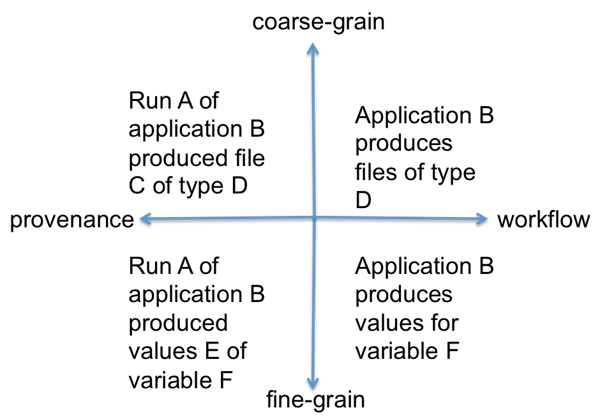
\includegraphics[keepaspectratio,alt={Dimensions of metadata}]{img/dimensions_of_metadata.png}}
\caption{Dimensions of metadata}
\end{figure}

\begin{figure}
\centering
\pandocbounded{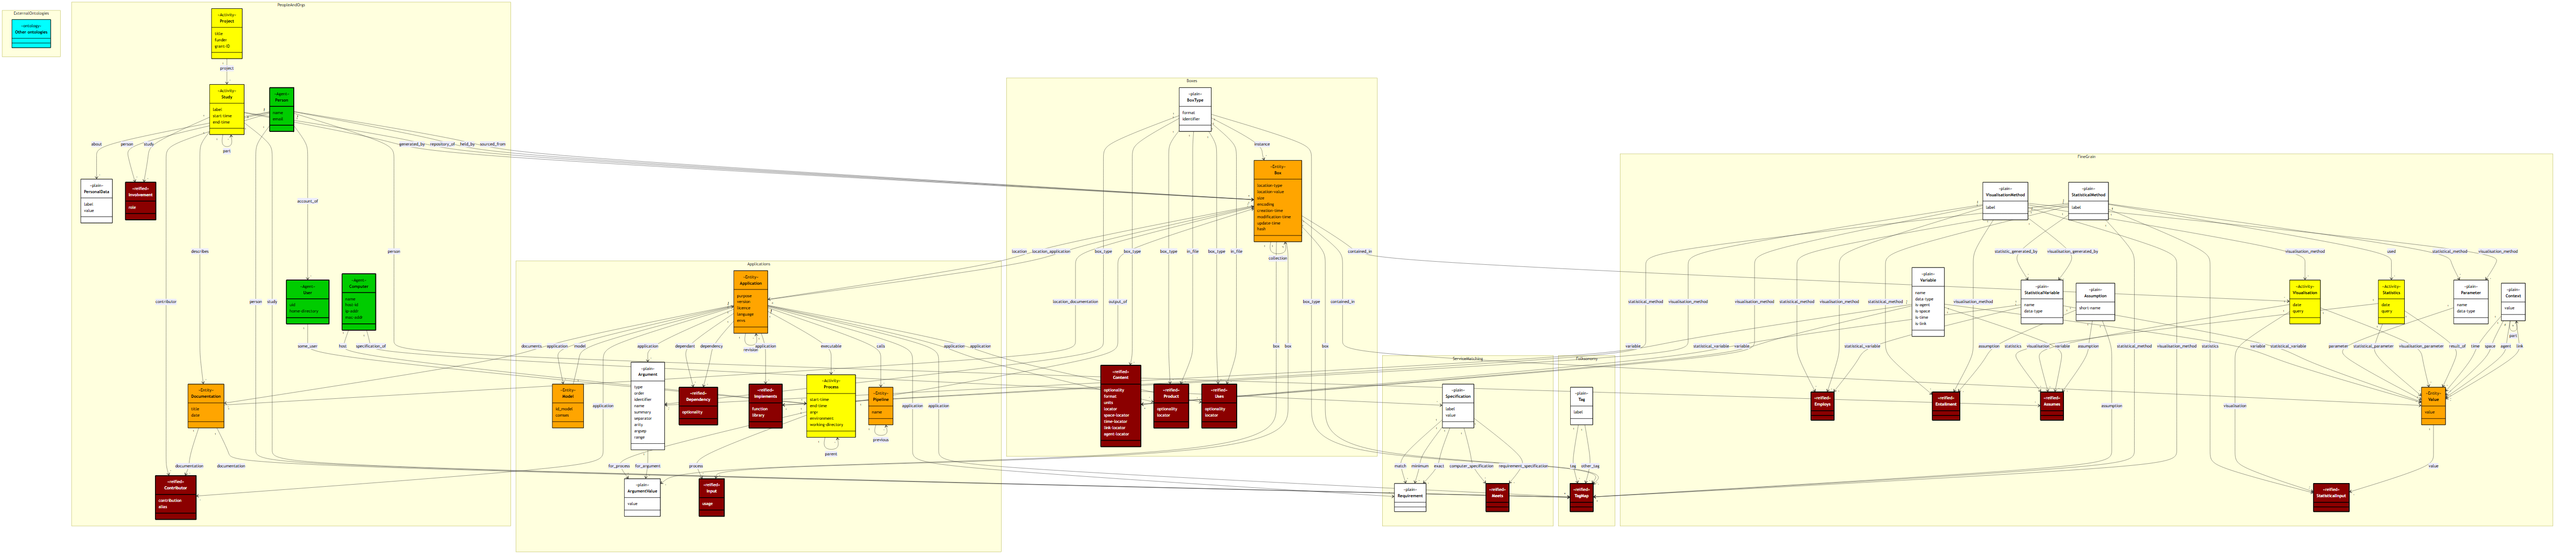
\includegraphics[keepaspectratio,alt={Metadata schema for MIRACLE. Boxes indicate tables, arcs represent relations, with `forked' arrowheads showing the `many' part of a many-to-one or many-to-many relationship. Tables are coloured in brown if they are breaking a many-to-many relationship (a reified relationship), with yellow, orange and green being used to denote specialisations from the PROV standard Activity, Entity and Agent classes respectively. Thick borders denote tables that are potentially autopopulated. Other tables are assumed to be entirely populated by users. Blue octagons show external databases/ontologies to which this one could be linked.}]{img/diagram-01.png}}
\caption{Metadata schema for MIRACLE. Boxes indicate tables, arcs
represent relations, with `forked' arrowheads showing the `many' part of
a many-to-one or many-to-many relationship. Tables are coloured in brown
if they are breaking a many-to-many relationship (a reified
relationship), with yellow, orange and green being used to denote
specialisations from the PROV standard Activity, Entity and Agent
classes respectively. Thick borders denote tables that are potentially
autopopulated. Other tables are assumed to be entirely populated by
users. Blue octagons show external databases/ontologies to which this
one could be linked.}
\end{figure}

With the schema now having a large number of tables, it is better to
consider it in parts. The schema visualisation document is now in a
format suitable for using C pre-processor commands to pull out various
subgraphs. The following are available:

\begin{itemize}
\item
  ALL: Show the entire schema.
\item
  ANALYSIS: Show the part of the fine grain pertaining only to analysis
  and visualisation.
\item
  EXTERNAL: Show the links to external ontologies.
\item
  FINEGRAIN: Show everything relating to fine grain metadata.
\item
  FOLKSONOMY: Show the tables that allow tagging.
\item
  PROJECT: Show information relating to metadata about projects.
\item
  PROV: Show tables capturing provenance metadata.
\item
  SERVICES: Show tables pertaining to service-provision and matching
  requirements against specifications.
\item
  WORKFLOW: Show tables relating to workflow.
\end{itemize}

The overview section now continues with an explanation of each subgraph
in turn, with consideration given to the degree of user interaction and
maintenance. The remainder of the document thereafter explains each
table in detail.

\section{Analysis}\label{analysis}

The subgraph for recording metadata about Analysis is shown in Figure 3.
Variables are metadata about the content of files, and may have several
Values. These Values may be visualised, and Statistics may be computed
using them. Statistics are computed using StatisticalMethods, and
Visualisations constructed using VisualisationMethods.
StatisticalMethods produce StatisticalVariables as outputs, which are
stored in the Values table as results-of Statistics. Statistics and
Visualisations are thus conceived as Activities in the PROV vocabulary
(Gao, Chen, and Du 2020).

When a user of the system has identified some statistics or
visualisations they want to be able to reuse in other studies or record
provenance about, as part of recording the activity, if the statistics
are not something already added by another user, they would make an
entry in the StatisticalMethods or VisualisationMethods tables. If
known, the user would also record any Assumptions Entailed by the
methods. This information is not a requirement, as the user may not have
relevant expertise to assert that a particular computation involves an
Assumption; however, this information can be added at any time by any
user. The Employs table can also be filled with data recording when one
Statistical- or Visualisation-Method uses a StatisticalVariable as
input.

Assumptions could be quite trivial -- in the most simple case, for
example, that a numeric Variable is assumed to be a cardinal (as opposed
to ordinal or nominal) when computing the mean of its Values. For other
statistics, Assumptions can record such things as whether the Variable
is normally distributed, or has constant variance.

Once an Assumption has been stated as Entailed by a Statistical- or
Visualisation-Method, it can be automatically inferred that Persons have
made Assumptions about Variables, where they have done Statistics or
Visualisations that use the Methods and Values of those Variables that
are returned by the queries used to get the raw data on which the
activities operated. The query is stored, along with the date made, in
order to avoid populating large relational tables recording the
Visualisations and Statistics that used Values as input data. Note that
Values may also be used to store Parameters and StatisticalVariables
that act to configure Visualisations and Statistics. These are captured
using the visualisation-parameter and statistical-parameter relations,
and the StatisticalInput table.

Visualisations are automatically inferred when the Box they are
contained-in has a BoxType with a VisualisationMethod in it. The Values
visualised (recorded in the VisualisationValue table) can be (possibly
somewhat dubiously) inferred from the Input to the Application that ran
the Process that created the Box, until such time as statistical tools
support logging this information in sufficient detail.

\begin{figure}
\centering
\pandocbounded{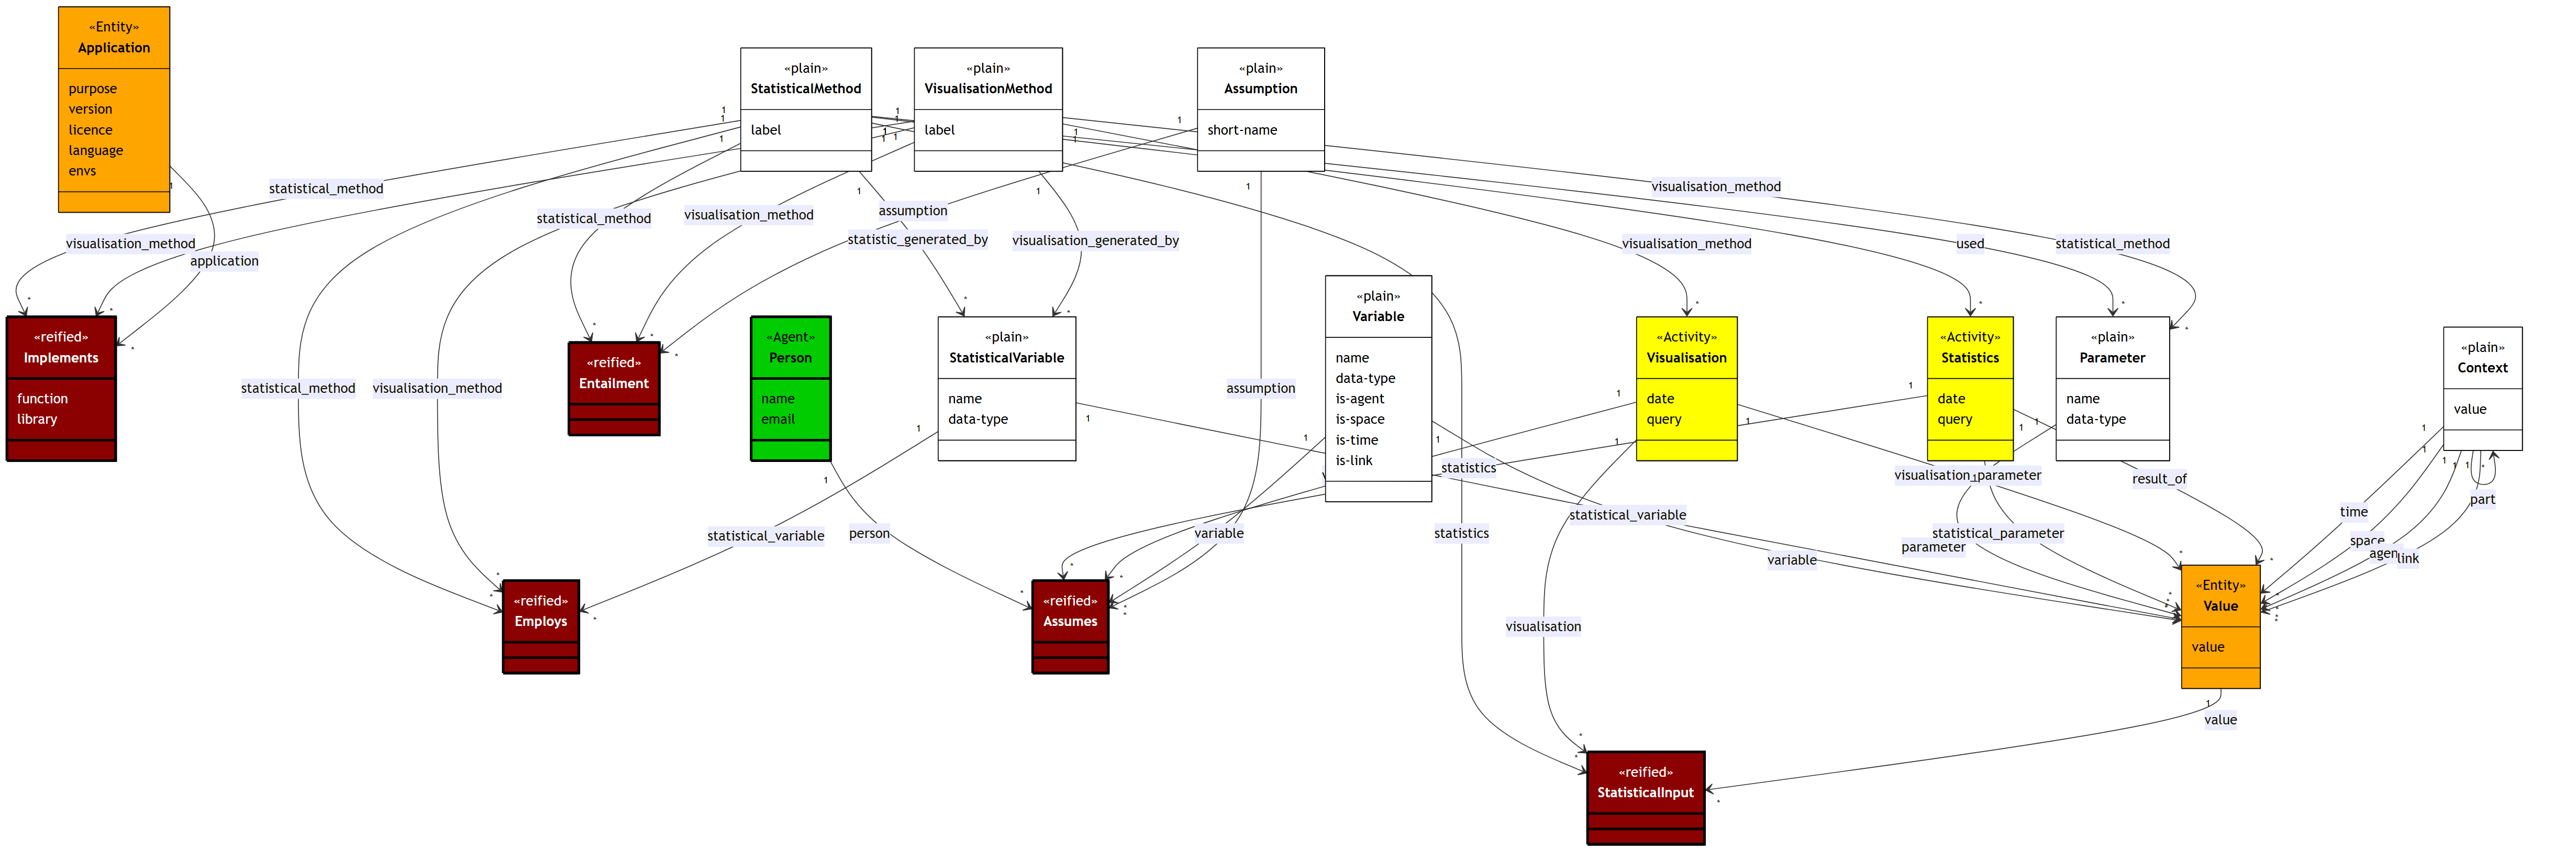
\includegraphics[keepaspectratio,alt={The analysis subgraph of the schema}]{img/diagram-02.png}}
\caption{The analysis subgraph of the schema}
\end{figure}

\subsection{External ontologies}\label{external-ontologies}

Though not explicitly noted in the tables, with the exception of OpenABM
(with which this schema has to integrate for the MIRACLE project),
various external ontologies and schemas are relevant, and could be
linked to if required. There are various ways such links could be
manifested (relational tables for example, implementing each of the blue
dashed lines in Figure 4), and those suggested are by no means
exhaustive. Neither is it necessarily the case that any specific
ontology or external schema is proposed or adopted. The following gives
examples of specific external links:

\begin{itemize}
\item
  Bib -- connection to a bibliographic database (e.g.~bibsonomy). Note
  that the Documentation table is intended to be quite generic, and
  include journal and conference articles as well as reports and code
  documentation.
\item
  Geo -- links to ontologies or databases containing geographical or
  spatial concepts, such as GeoSparql and WGS84. The idea here is that
  we may want to link various table entries to external geographical
  databases, for example, to say that a Study pertained to a particular
  region, or that a Box is a GIS file.
\item
  OpenABM -- this is linking back to the CoMSES-Net archive of
  agent-based models, and is essential in order to identify which model
  these metadata are describing the output analysis of. (Although in
  principle, the system described could be applied to any stage of
  modelling, including setting up the model files, running the model and
  analysing the output, the focus of the MIRACLE project is specifically
  on the output analysis.)
\item
  Services -- links to vocabularies describing the requirements of
  applications and capabilities of service-providers. Where WSDL and
  OWL-S were once the natural reference points here, most service
  description in practice has since moved to REST-style APIs described
  using OpenAPI (formerly Swagger), which is now the de facto standard
  for machine-readable service interfaces. OpenAPI lacks OWL-S's
  semantic-reasoning ambitions, but its wide tooling support and
  adoption make it a more practical link for automatic discovery of
  applications and services, including their input and output
  specifications.
\item
  SocialWeb -- we may want to allow people to link to social web tools
  such as ResearchGate, LinkedIn, Facebook and Twitter. The FOAF
  ontology also has attributes that we can draw on, and includes
  vocabulary for modelling social web links.
\item
  Workflow -- workflow-related ontologies. Standards in this space
  remain relatively immature. The Common Workflow Language (CWL) has
  emerged as the most widely adopted tool-agnostic specification for
  describing computational workflows, and is a natural candidate for
  linking here. Other approaches to modelling workflows, such as
  Petri-Nets and various business process modelling ontologies, remain
  potentially relevant, though PROV-O may be a more durable choice than
  domain-specific alternatives for capturing workflow provenance in
  particular (Herschel, Diestelkämper, and Ben Lahmar 2017).
\end{itemize}

\begin{figure}
\centering
\pandocbounded{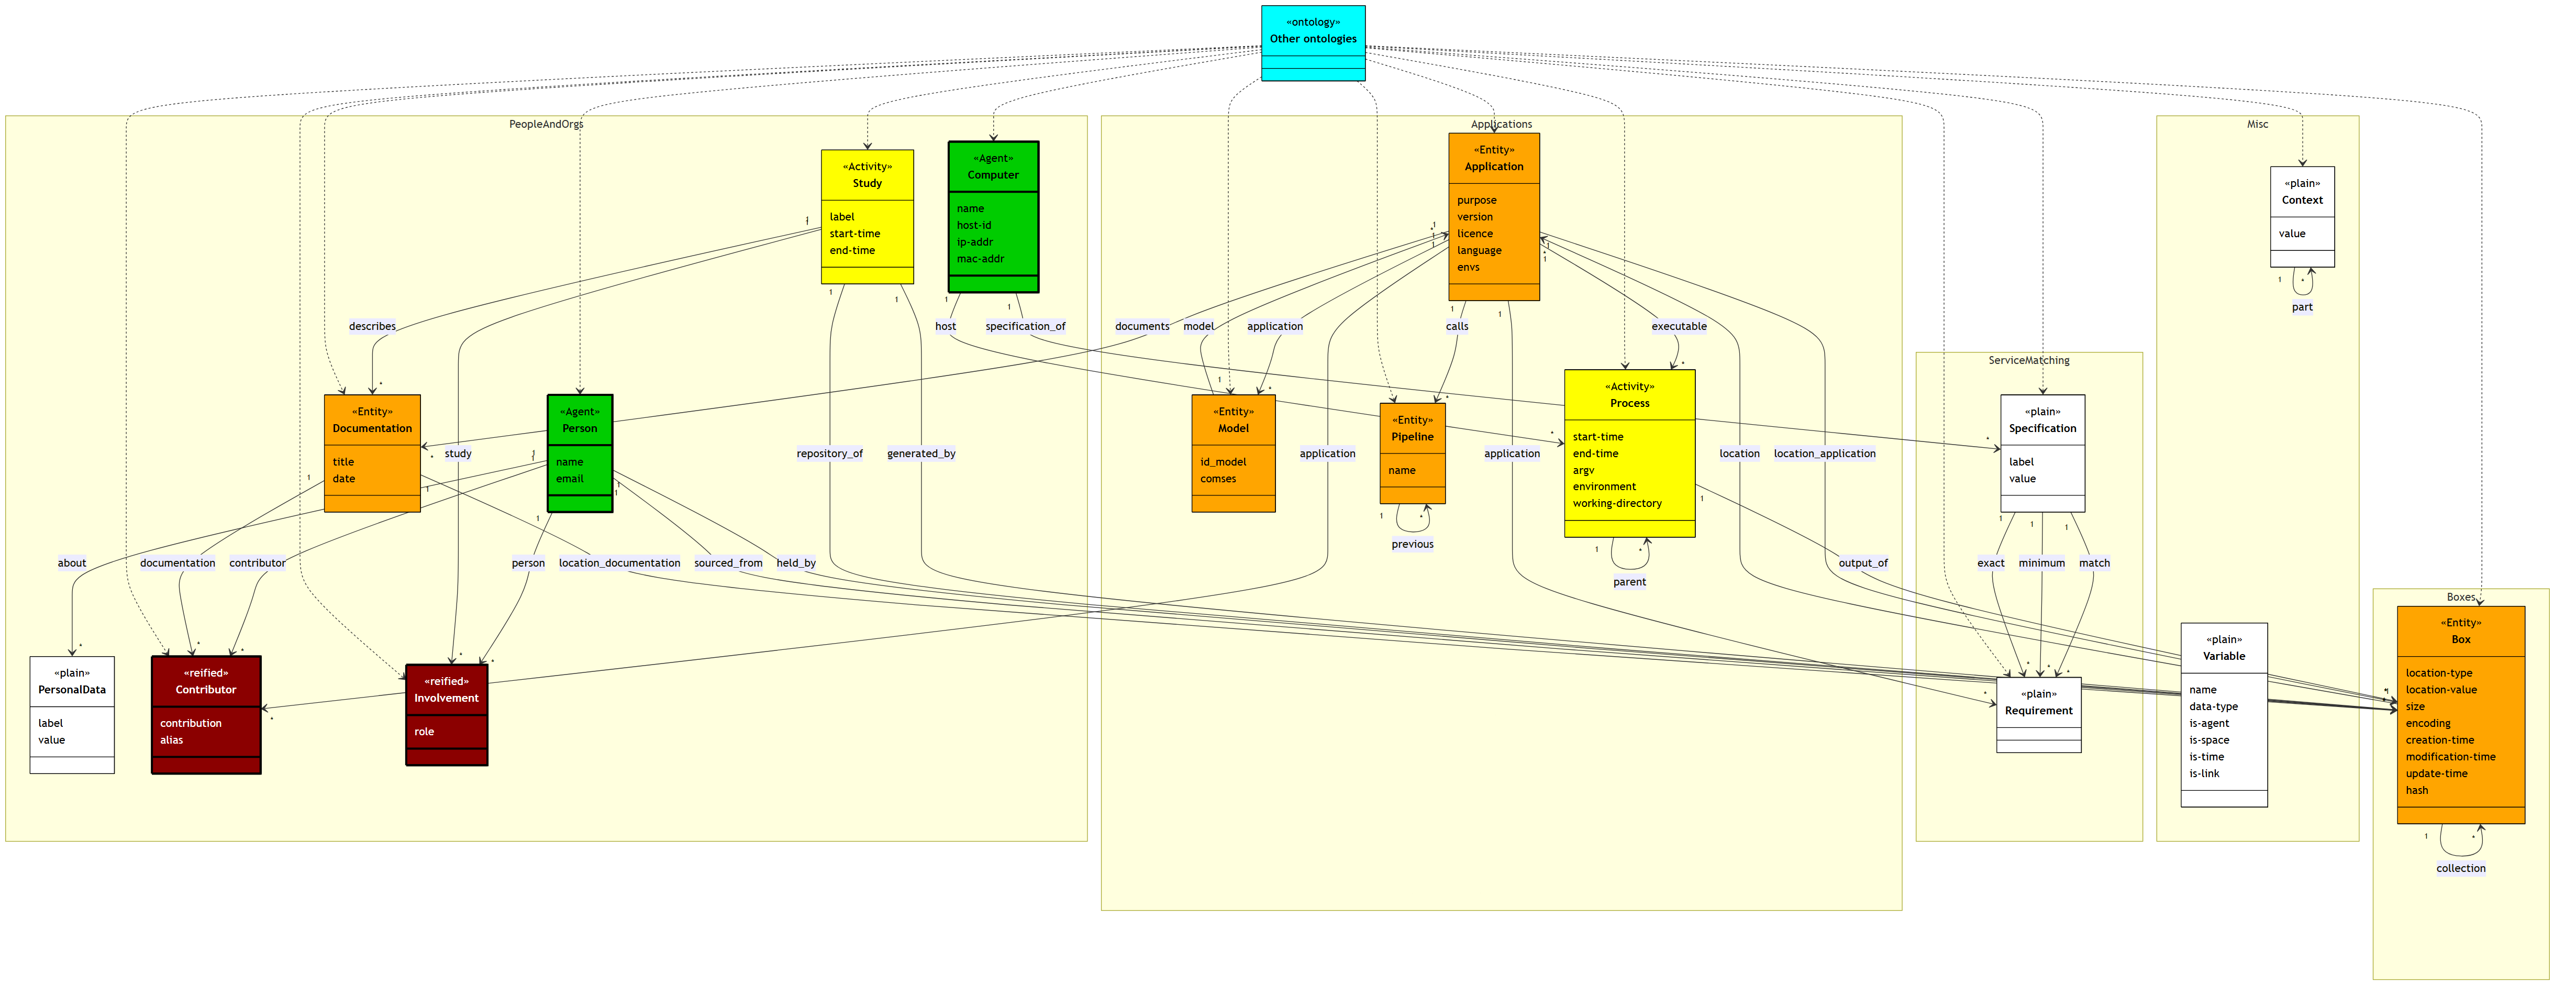
\includegraphics[keepaspectratio,alt={Subgraph showing possible tables that external ontologies could link to, and some relationships between them.}]{img/diagram-03.png}}
\caption{Subgraph showing possible tables that external ontologies could
link to, and some relationships between them.}
\end{figure}

In terms of maintenance, provision for making the links to external
databases would require users to supply the relevant information, except
where specifically supported databases provided an API allowing us to
query them for possibly relevant data to link to.

\subsection{Fine grain}\label{fine-grain}

The fine grain metadata is information about the contents of files,
including visualisations, and values of variables (Figure 5). Much of
this has been covered already in the Analysis section above, but here we
show how Boxes are disaggregated from a provenance perspective through
saying that Values and Visualisations are contained-in them, and from a
workflow perspective through saying that BoxTypes have Variables and
VisualisationMethods as their content. The provenance side can be
populated automatically, but the workflow metadata would need to be
provided by the user when describing an Application they were making
available to the system: specifically, the user will need to describe
the inputs and outputs of each application, and for each associated
BoxType, provide details of Variables and VisualisationMethods given as
content. For some file formats, autodetection may assist with populating
the Variable table -- e.g.~given an example of a CSV file used by or
generated by an application, a header row could be used to suggest names
for Variables they supply.

\begin{figure}
\centering
\pandocbounded{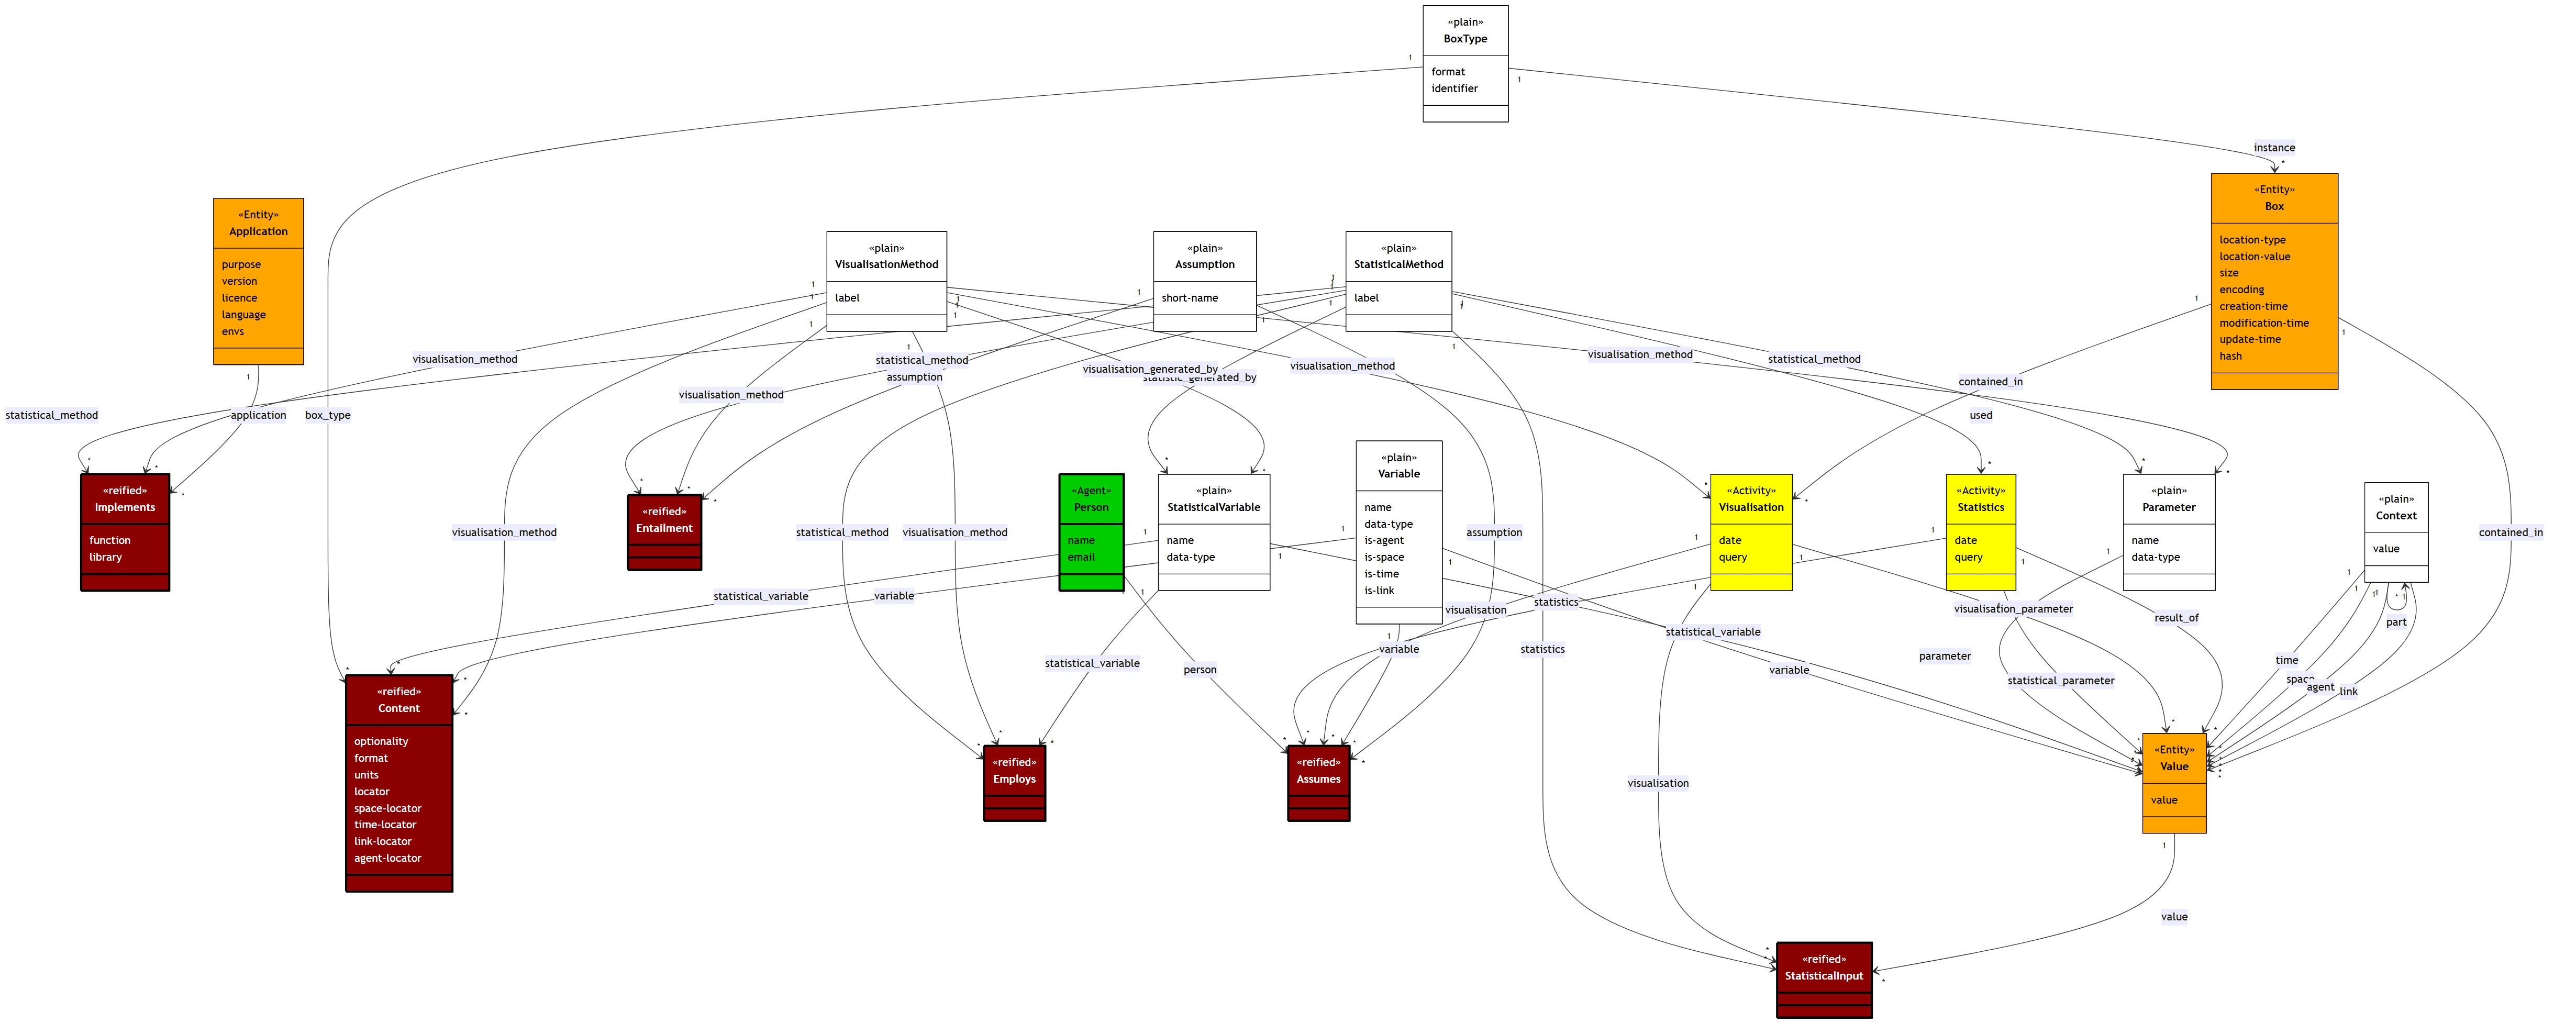
\includegraphics[keepaspectratio,alt={Subgraph showing the fine grain metadata tables}]{img/diagram-04.png}}
\caption{Subgraph showing the fine grain metadata tables}
\end{figure}

\subsection{Folksonomy}\label{folksonomy}

Folksonomies are informal ontologies developed by a user communities,
with tagging being a pretty much standard way in which this is achieved.
It is not proposed to enrich that here. In Figure 6, the tables thought
most likely to be of interest for users to tag are depicted, though this
needn't be exhaustive. Each of the arcs from the Tag table would need a
relational table to break the jmany-many relationship between tags and
the concepts they are applied to.

\begin{figure}
\centering
\pandocbounded{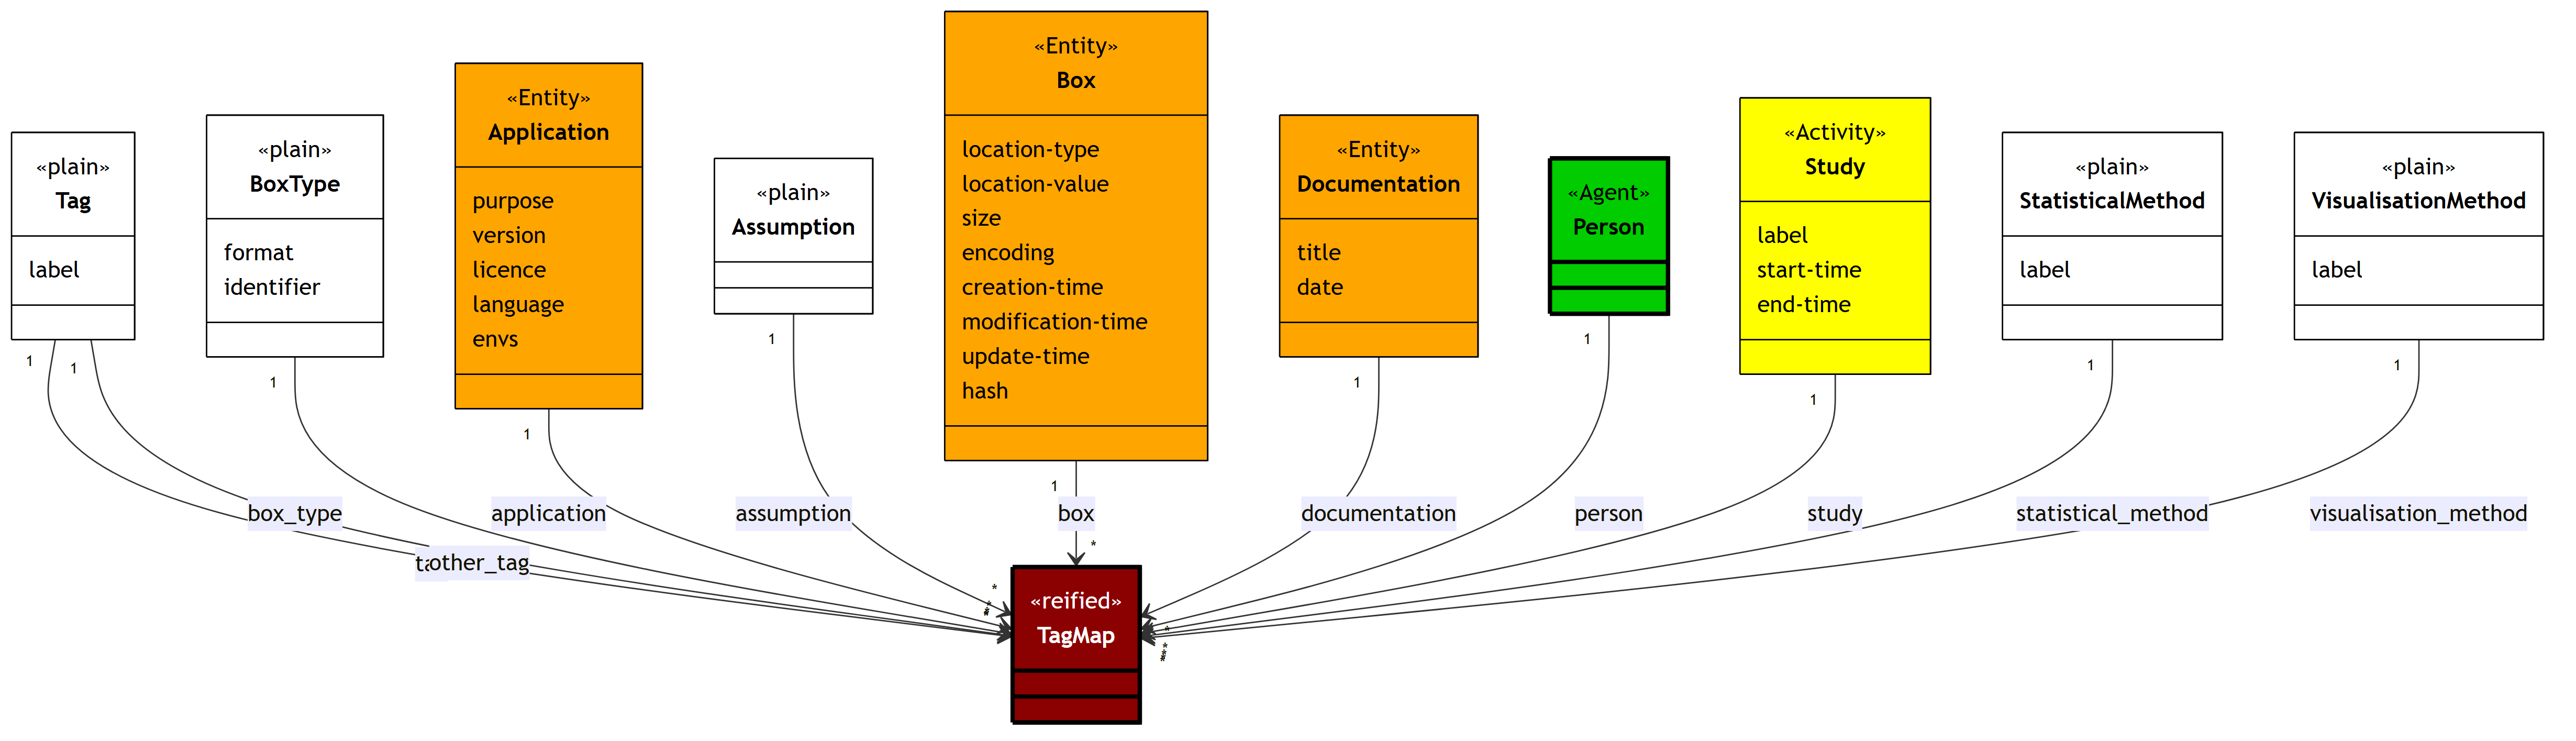
\includegraphics[keepaspectratio,alt={Folksonomy subgraph. Each of the arcs would itself be a reified table showing the application of Tags to tables.}]{img/diagram-05.png}}
\caption{Folksonomy subgraph. Each of the arcs would itself be a reified
table showing the application of Tags to tables.}
\end{figure}

\subsection{Project}\label{project}

\begin{figure}
\centering
\pandocbounded{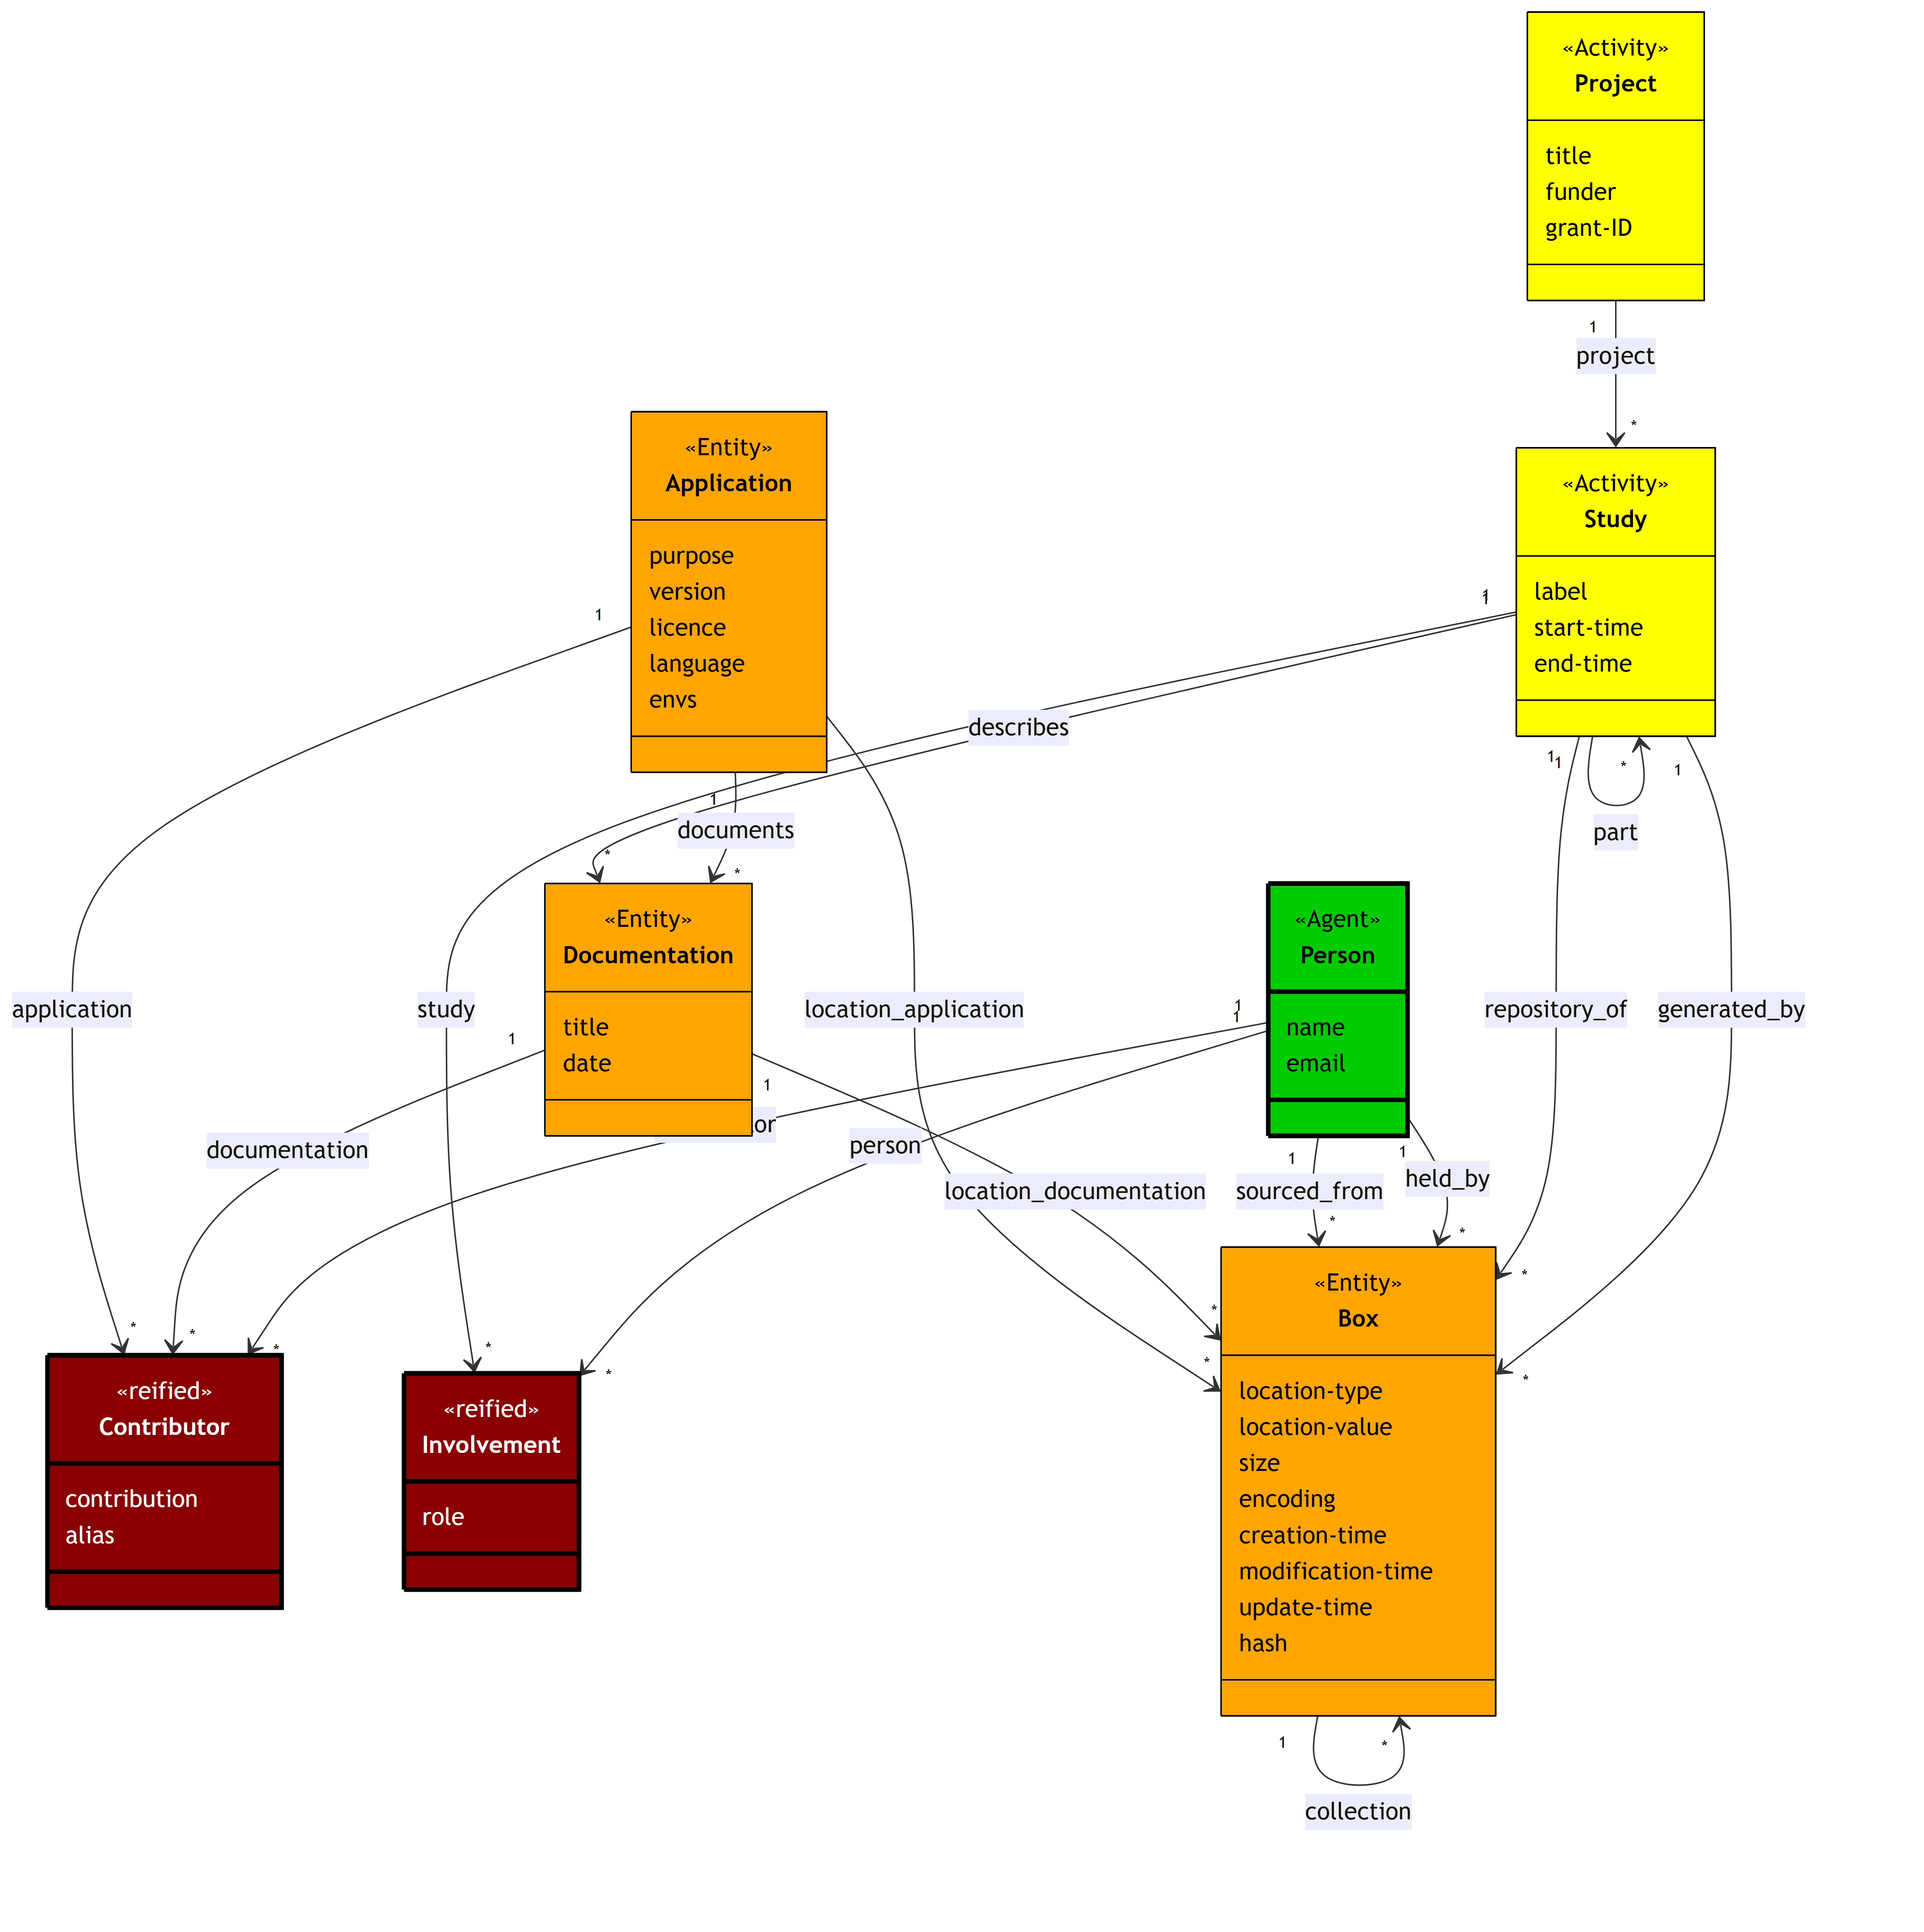
\includegraphics[keepaspectratio,alt={Subgraph capturing metadata about projects}]{img/diagram-06.png}}
\caption{Subgraph capturing metadata about projects}
\end{figure}

Project metadata is largely for users to enter, and previously may have
been regarded as unduly onerous. With the advent of large language
models, much of this metadata might be automatically generated. It is
provided to facilitate users in understanding how simulation output data
relates to publications (which would appear in the Documentation table),
and specific pieces of work (Study table). The Study might be the most
important table for users to complete, as this, by its association with
Boxes allows collection of simulation outputs in useful groups.

\subsection{Provenance}\label{provenance}

\begin{figure}
\centering
\pandocbounded{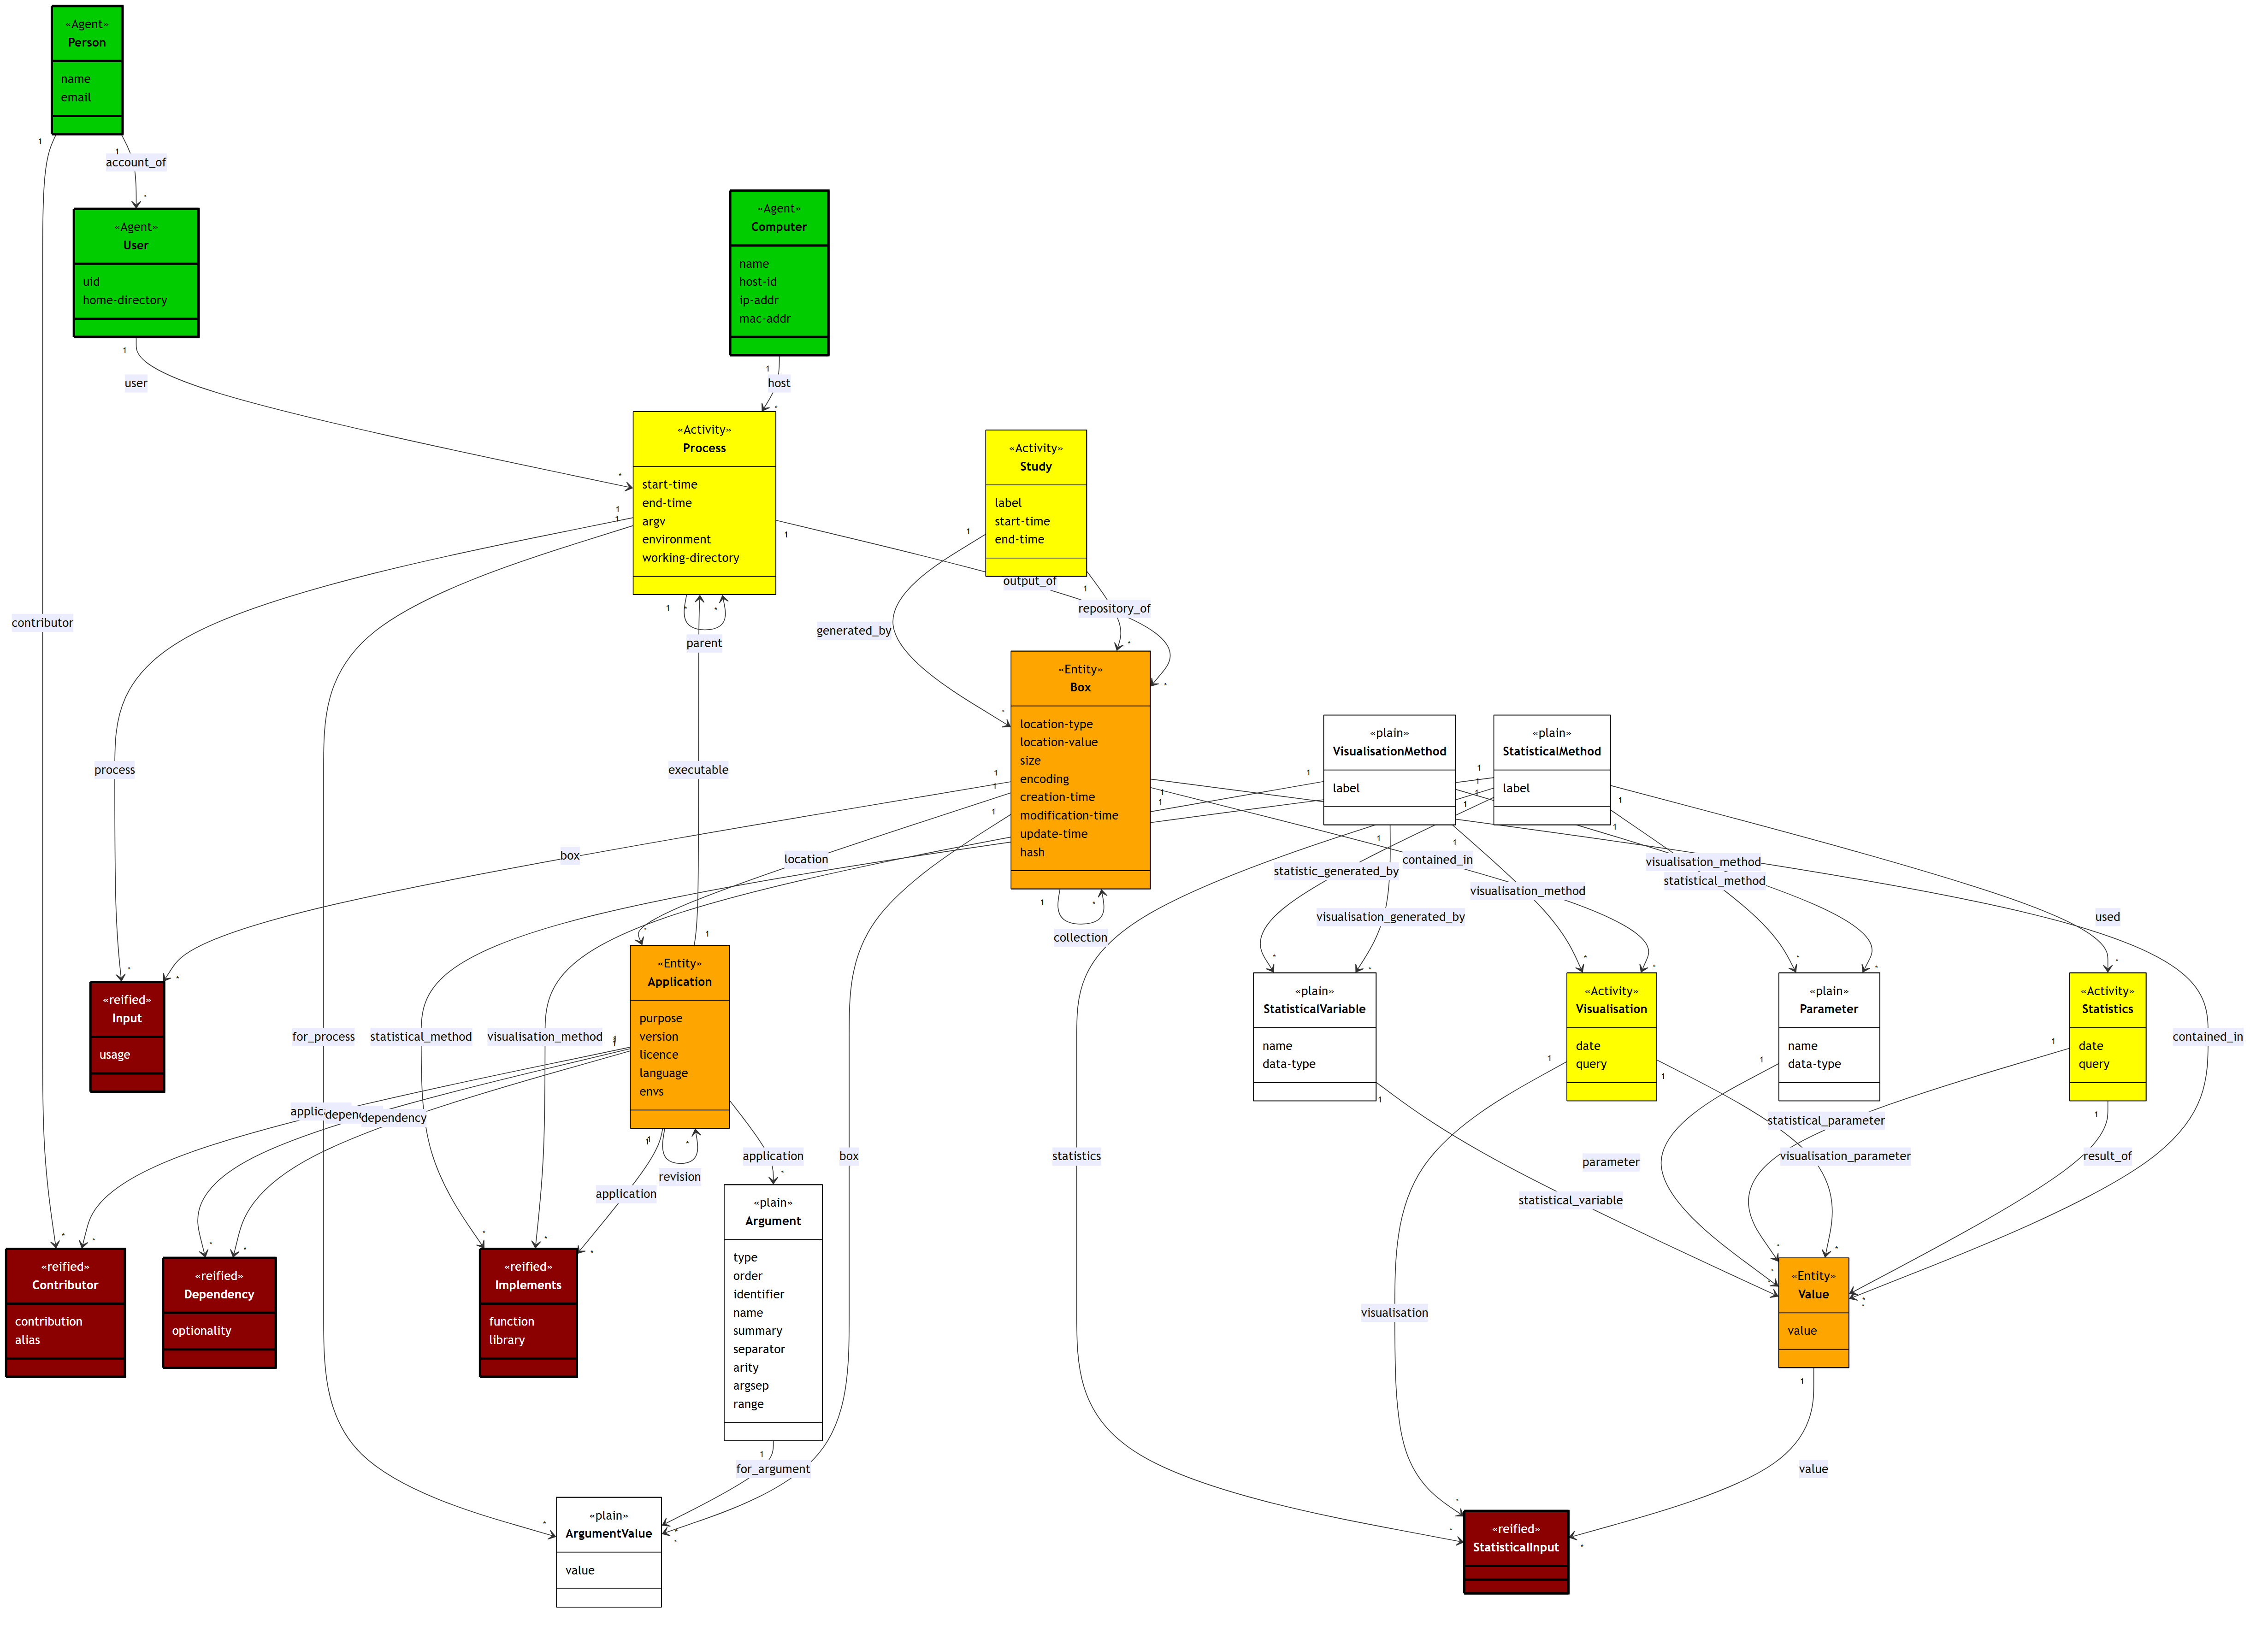
\includegraphics[keepaspectratio,alt={Provenance subgraph}]{img/diagram-07.png}}
\caption{Provenance subgraph}
\end{figure}

Provenance is very much at the heart of the system, with an important
role in recording how results from a model presented in journal articles
are produced (Oliveira, Oliveira, and Braganholo 2018). Most of the
tables here are autopopulated, as particularly for large scale analyses,
user entry is an unrealistic goal. The system therefore needs to act as
a wrapper around the scripts and tools (Applications) used to process
the raw output from the simulation (which is the starting point of the
MIRACLE project (Jin et al. 2017)) into the result used as part of an
article. At the coarse grain, the central activity is the Process, which
is a record of all relevant information of a process that ran on a
Computer. This includes anything needed to replicate that Process under
the same circumstances: the input files it used, command-line arguments,
environment variables (essentially, anything that might affect its
behaviour), and the output files it generated, the importance of which
is illustrated by the challenges encountered when replicating the
analysis of outputs from a social simulation of biodiversity
incentivisation (Polhill et al. 2017).

The need for cross-platform support means that it is difficult to draw
on standards for these. Different operating systems, and even different
commands within the same operating systems, use different conventions
for processing input on the command line, and input and output
redirection. The Argument table attempts to record all relevant details
about command-line arguments, allowing ArgumentValues to be inferred
from a specific command-line instruction activating a Process. This is
important in avoiding the need for users to supply too much information
each time they run an Application.

Batch-file processing is assumed at the coarse grain; where processes
involve user interaction that might affect the behaviour, automatic
capture of provenance data would be extremely challenging. Whilst GUIs
might be used during exploratory analysis of simulation output data,
ultimately for reproducibility of results and keeping records of
activities done (Pritchard and Wicenec 2025), these must ultimately be
manifested as scripts that can be run in batch mode, once a decision is
taken that a particular analysis step needs to be recorded as an
application. Applications that only support GUI interaction can
therefore not be supported (and arguably should be derided as virtually
useless for any scientific endeavour -- assuming repeatability is a
desirable attribute of that work).

At the fine-grain, Statistics and Visualisations are the central
activities. Again, although GUI interaction cannot be supported,
command-line interaction potentially could. Parameters and
StatisticalInput would need to be recorded, and the raw data on which
the activities operate captured somehow in a query allowing the same set
of data to be operated on. Recording the date at which the query was
made is therefore important, especially if Values of Variables are
subsequently populated that might affect the ability of future analyses
to reuse the same data. A short-cut might be to store the date a Value
was generated in the Values table, but since this table is expected to
be `virtual' (in that a supporting system would gather relevant data
from the raw data files), the date can be captured from the dates of the
Processes generating the Boxes in which the Values appear, or the date
at which the Statistics were computed if the Value is a
StatisticalInput.

\subsection{Services}\label{services}

\begin{figure}
\centering
\pandocbounded{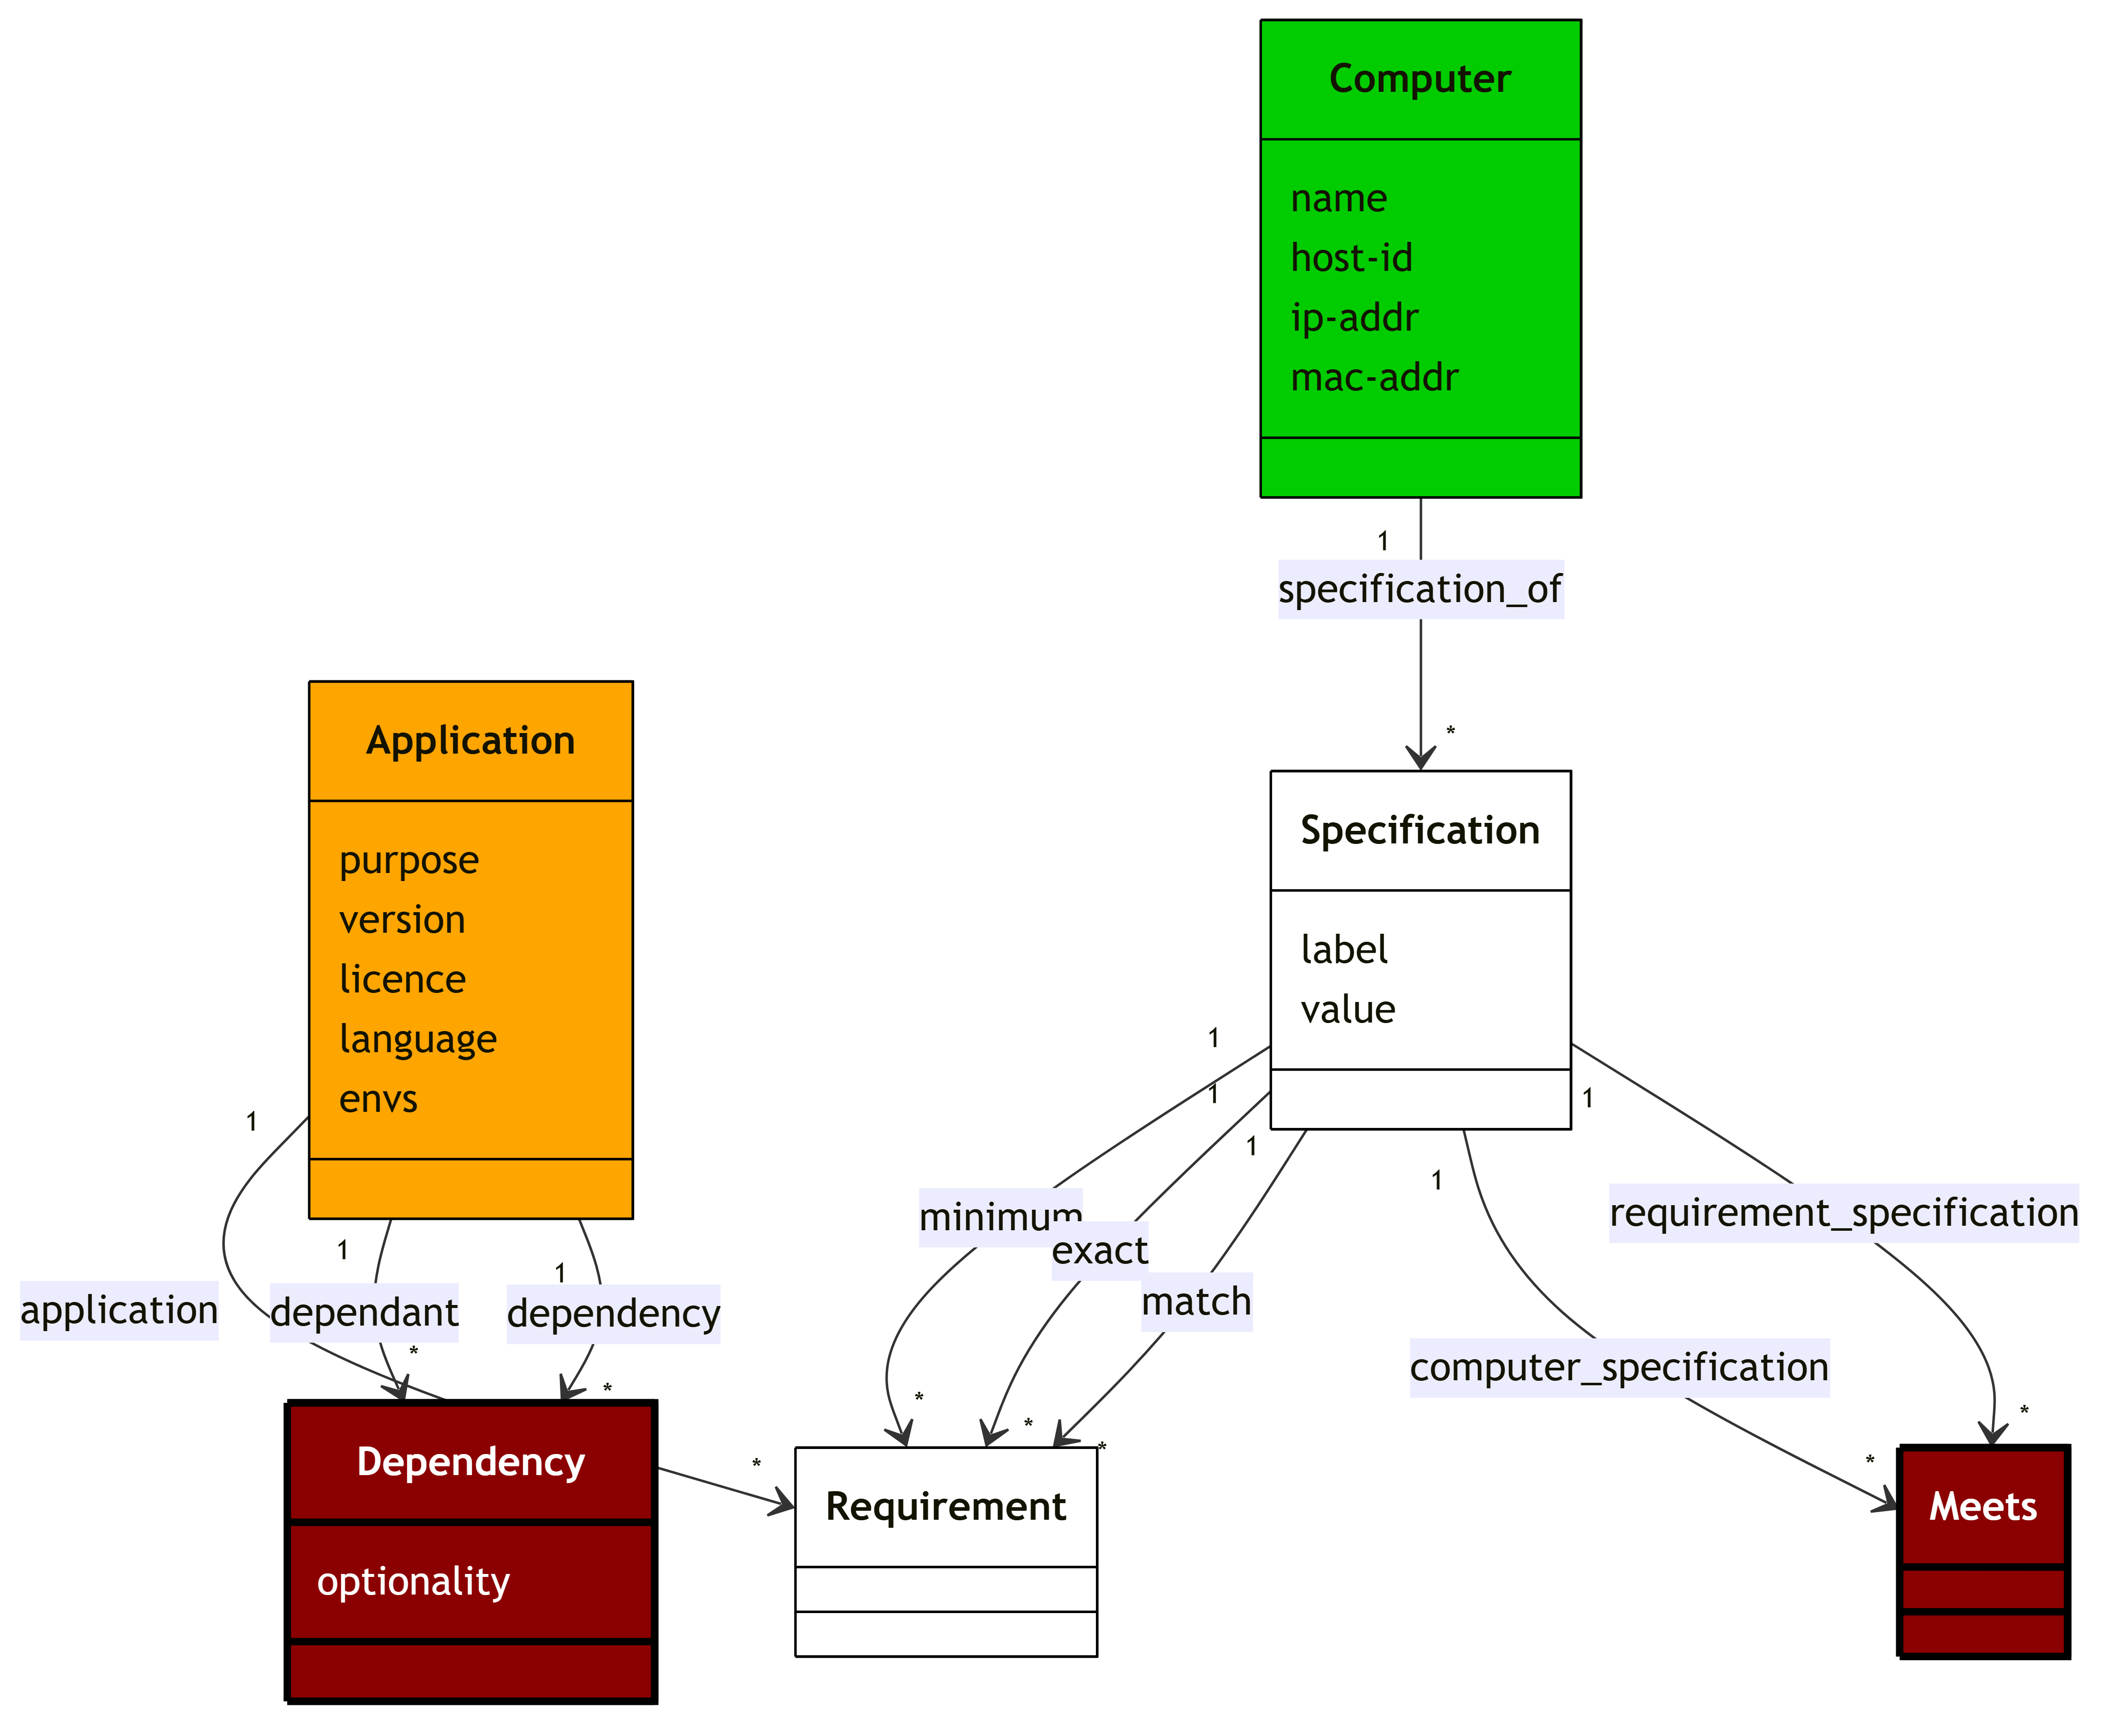
\includegraphics[keepaspectratio,alt={Services subgraph}]{img/diagram-08.png}}
\caption{Services subgraph}
\end{figure}

The services part of the graph depicted in Figure 9 provides a simple
model intended to be used to determine whether an Application can be run
on a Computer. This involves checking the Requirement Specifications of
the Application (and recursively of any Dependencies) against the
Specifications of a Computer. Requirements can be specified in one of
three ways -- for numeric Requirement Specifications, a `minimum'
Requirement must be exceeded by the Specification of the Computer (e.g.
for RAM). For all types of Requirement Specifications, an `exact'
Specification must be equal (an example might be the OS -- if the
Application has very specific demands), whilst a `match' Specification
is a regular expression that the Specification of the Computer must
match. The results are stored in the Meets reified relationship.

A more sophisticated implementation would wrap each Application in a web
service. This would also be more secure if responsibility for providing
Applications as web services was in the hands of their developers -- we
would then not be uploading Applications to our system, but instead
sending data for processing by other servers, and capturing metadata
about these interactions. The services architecture could then draw much
more heavily on standard web services ontologies, such as OWL-S and
WSDL.

\subsection{Workflow}\label{workflow}

\begin{figure}
\centering
\pandocbounded{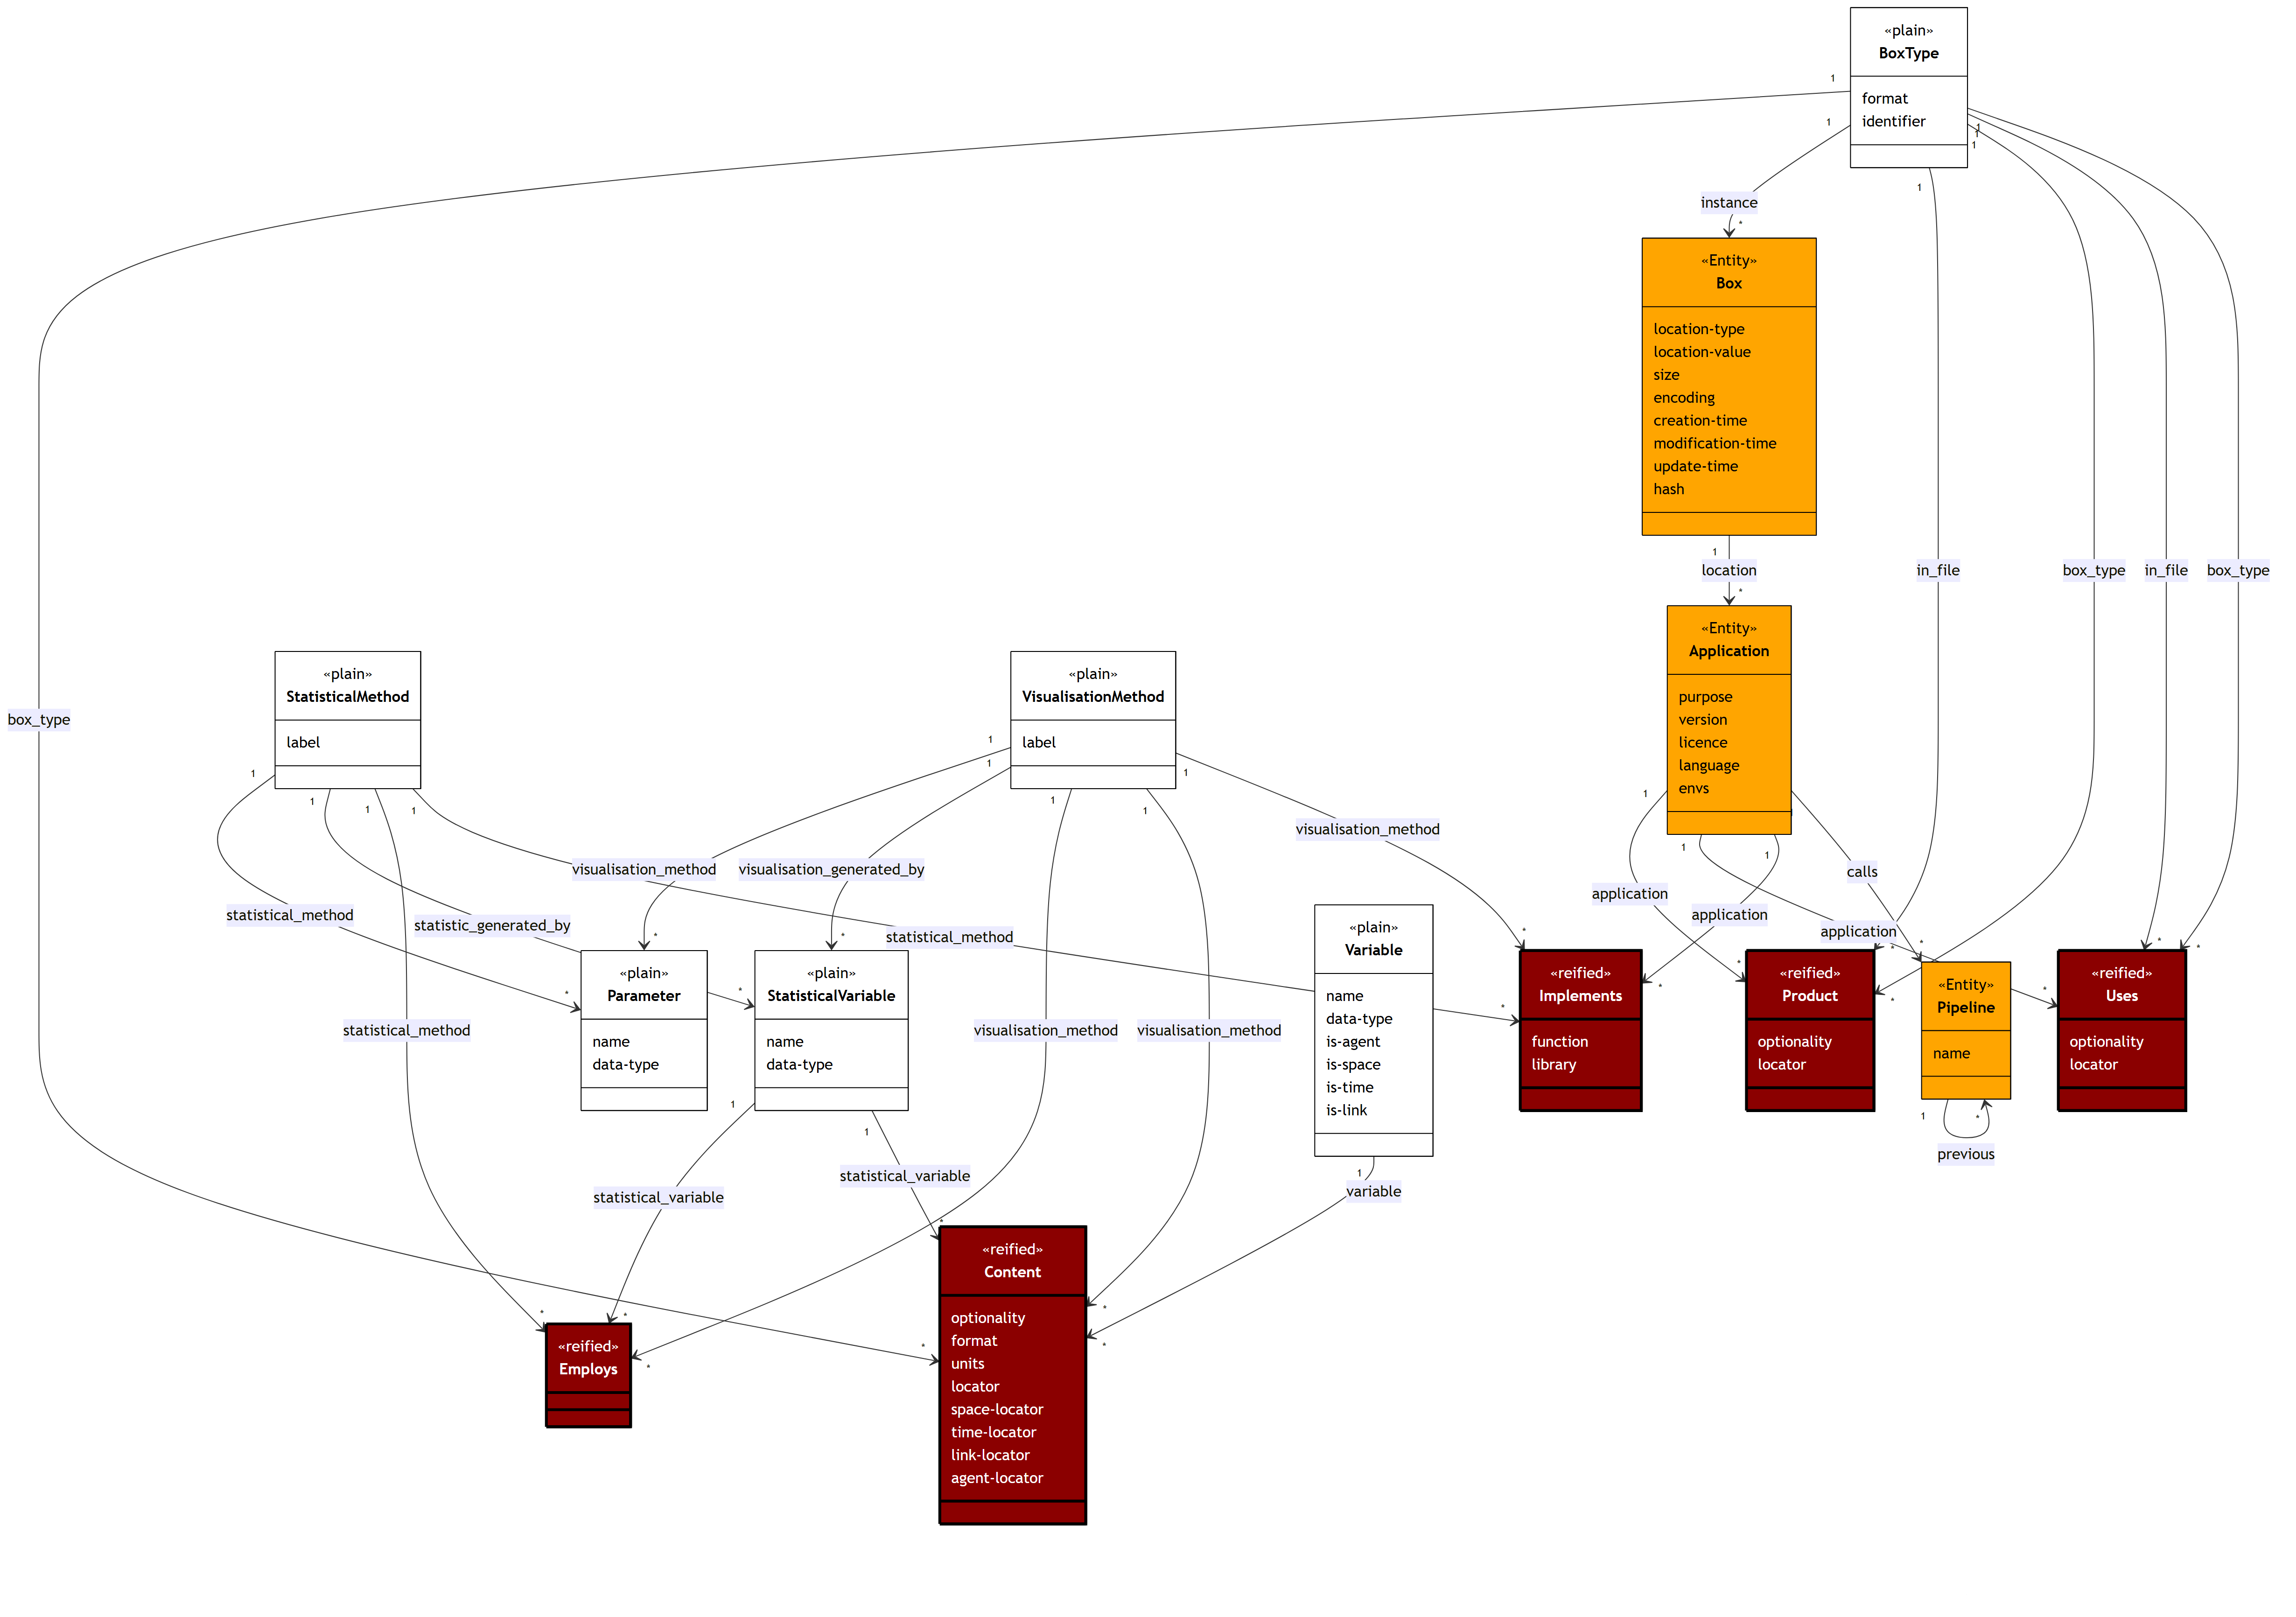
\includegraphics[keepaspectratio,alt={Workflow subgraph}]{img/diagram-09.png}}
\caption{Workflow subgraph}
\end{figure}

The standard workflow model provides prescriptive `recipes' for
undertaking specific procedures (Atkinson et al. 2017). Though we are
interested in that here, and have provided a rudimentary sequence-based
Pipeline table to handle that, we are also interested in providing
support for exploring what `could be done' given a current set of
circumstances, and `what needs to be done' before running an
Application. For example, suppose we are interested in getting a Value
for a particular Variable. Then we can see which BoxTypes have that
Variable in their Content, and which Applications have the BoxType as a
Product. If the BoxTypes those Applications Use have no instances, then
we can find Applications that have the Uses BoxTypes as their Product,
and so on. We can also search for Pipelines that have the required
Product by exploring the Products of the last element of each Pipeline's
list-based structure, and checking the Uses of the first element.

This way, it should be possible, given a set of raw simulation outputs,
to search for sequences of Applications to apply that generate a
particular desired Visualisation(Method). Using the Provenance
infrastructure, it would also be possible to explore how other users
have chosen to do it in the past.

\section{Detailed specifications}\label{detailed-specifications}

All tables have uniquely specified ID fields as primary keys, unless
they are associative tables. All tables with have a name field. This is
free form text and not always present. This identifies a relation,
however this is not guaranteed to be unique or even present. It is there
to help primarily in readability when trying to extract information from
this database and may contain a human readable label for the relation.
For instance, for the definition of an argument, this would be the
argument name. All tables will have a description field
(dc:description). This field has been included to allow the introduction
of free form documentary text. It is strongly advised that should the
opportunity arise, then such text is supplied. The authors recommend
this practice as it forms a useful means of documenting job control code
in its own right, used to run these large scale models. Each table also
has a creator/modifier field, and a corresponding created and modified
date time field. Although most databases record this kind of metadata,
we have made it explicit and expect these fields to be populated
automatically. This a deliberate attempt to make this interface database
software agnostic. Note that date fields should be stored as strings
conforming to the ISO 8601 date format, not in the native format of the
database. This is recommended best practice according to the Dublin Core
Metadata Initiative.{[}\^{}1{]} The remaining attribute that is always
included in each relation is the "about" column. This we have pinched
directly from RDF and uniquely identifies a triple in RDF (Hartig and
Zhao 2010). Although currently optional, we intend this to uniquely
identify the relationship within our database. The form of this normally
some kind of IRI. This will allow inward referencing of the provenance
and metadata resource from other standardised resource software that
recognizes IRIs.

\subsubsection{Attributes}\label{attributes}

\begin{longtable}[]{@{}
  >{\raggedright\arraybackslash}p{(\linewidth - 8\tabcolsep) * \real{0.2000}}
  >{\raggedright\arraybackslash}p{(\linewidth - 8\tabcolsep) * \real{0.2000}}
  >{\raggedright\arraybackslash}p{(\linewidth - 8\tabcolsep) * \real{0.2000}}
  >{\raggedright\arraybackslash}p{(\linewidth - 8\tabcolsep) * \real{0.2000}}
  >{\raggedright\arraybackslash}p{(\linewidth - 8\tabcolsep) * \real{0.2000}}@{}}
\toprule\noalign{}
\begin{minipage}[b]{\linewidth}\raggedright
Attribute
\end{minipage} & \begin{minipage}[b]{\linewidth}\raggedright
Description
\end{minipage} & \begin{minipage}[b]{\linewidth}\raggedright
Standards
\end{minipage} & \begin{minipage}[b]{\linewidth}\raggedright
Validation
\end{minipage} & \begin{minipage}[b]{\linewidth}\raggedright
Automation
\end{minipage} \\
\midrule\noalign{}
\endhead
\bottomrule\noalign{}
\endlastfoot
name & A documentary name for the relation or entity & None & None. May
or may not be present & None \\
description & Short text to use to summarise what the argument is & None
& String & None \\
about & A unique resource identifier. This field will allow inward
linking from any external resource that allow IRIs & RFC 3987 and RFC
4622 & IRI & None \\
creator & Who created this particular set of attributes making up this
relation & dc:creator & String & Should be done by the agency that has
implemented the SSREPI interface. This will be the computer user \\
created & When this document was created & dc:created, ISO8601 & logical
date and time validation & Should be done by the agency that has
implemented the SSREPI interface. This will be the computer user \\
modifier & Who created this particular set of attributes making up this
relation & dc:creator & String & Should be done by the agency that has
implemented the SSREPI interface. This will be the computer user \\
modified & When this document was created & dc:modified, ISO8601 &
Logical date and time validation. Must come after the date of creation.
& Should be done by the agency that has implemented the SSREPI
interface. This will be the computer user \\
\end{longtable}

\subsection{Annotation}\label{annotation}

This is not shown in the above diagrams. This is database entry that can
annotate any relation in this database. This can be used to flag certain
properties, or record information about a given set of rows. Such
properties will be recorded in a JSON format for the purposes
validation.

\subsection{Standards}\label{standards}

JSON for the annotation values. SQL for row restriction.

\subsection{Automation}\label{automation}

There is an entry which documents a database query (if suitable) that
will document the rows affected. It is up to the standard implementor
whether such queries will be allowed to be performed automatically. We
are recommending only statements that refer to the Box table should be
allowed to stop the possibility of SQL injections.

\subsubsection{Attributes}\label{attributes-1}

\begin{longtable}[]{@{}
  >{\raggedright\arraybackslash}p{(\linewidth - 8\tabcolsep) * \real{0.2000}}
  >{\raggedright\arraybackslash}p{(\linewidth - 8\tabcolsep) * \real{0.2000}}
  >{\raggedright\arraybackslash}p{(\linewidth - 8\tabcolsep) * \real{0.2000}}
  >{\raggedright\arraybackslash}p{(\linewidth - 8\tabcolsep) * \real{0.2000}}
  >{\raggedright\arraybackslash}p{(\linewidth - 8\tabcolsep) * \real{0.2000}}@{}}
\toprule\noalign{}
\begin{minipage}[b]{\linewidth}\raggedright
Attribute
\end{minipage} & \begin{minipage}[b]{\linewidth}\raggedright
Description
\end{minipage} & \begin{minipage}[b]{\linewidth}\raggedright
Standards
\end{minipage} & \begin{minipage}[b]{\linewidth}\raggedright
Validation
\end{minipage} & \begin{minipage}[b]{\linewidth}\raggedright
Automation
\end{minipage} \\
\midrule\noalign{}
\endhead
\bottomrule\noalign{}
\endlastfoot
id\_annotation & Unique key & None & Must be unique & Automated by the
instantiating framework \\
json & json describing the values of the records being annotated. & None
& Must be unique & Automated by the instantiating framework \\
sql & The SQL describing the range of records affected. This could be a
single rows from single or multiple tables. BEWARE OF SQL CODE INJECTION
when considering using this field & None & Must be unique & Automated by
the instantiating framework \\
\end{longtable}

\subsubsection{Relationships}\label{relationships}

None.

\section{References}\label{references}

\section{Application}\label{application}

\subsection{Description}\label{description}

An Application is something that can be run by the user to generate or
analyse simulation output.

\subsection{Standards}\label{standards-1}

\texttt{PROV:Entity}. Note the potential confusion. An Application is
something that has the potential to be an Activity (in the PROV sense)
in the form of a Process. However, PROV only deals with the past, not
with potential. The Application is a file somewhere, and hence an
Entity.

\subsection{Automation}\label{automation-1}

Most of this table is expected to be populated by the user.

\subsection{Attributes}\label{attributes-2}

\begin{longtable}[]{@{}
  >{\raggedright\arraybackslash}p{(\linewidth - 4\tabcolsep) * \real{0.2326}}
  >{\raggedright\arraybackslash}p{(\linewidth - 4\tabcolsep) * \real{0.1860}}
  >{\raggedright\arraybackslash}p{(\linewidth - 4\tabcolsep) * \real{0.5814}}@{}}
\toprule\noalign{}
\begin{minipage}[b]{\linewidth}\raggedright
Field
\end{minipage} & \begin{minipage}[b]{\linewidth}\raggedright
Property
\end{minipage} & \begin{minipage}[b]{\linewidth}\raggedright
Value
\end{minipage} \\
\midrule\noalign{}
\endhead
\bottomrule\noalign{}
\endlastfoot
ID\_APPLICATION & Type & TEXT \\
& Description & Unique key \\
& Standards & None \\
& Validation & Must be unique \\
& Automation & Automated by the instatiating framework \\
PURPOSE & Type & TEXT \\
& Description & Description of the purpose of the application \\
& Standards & ? \\
& Validation & Free text \\
& Automation & None \\
VERSION & Type & TEXT \\
& Description & Version ID for the application \\
& Standards & dc:? \\
& Validation & String (e.g.~CHAR(32)) \\
& Automation & None \\
LICENCE & Type & TEXT \\
& Description & Software licence for the application \\
& Standards & dc:license \\
& Validation & Free text with the option to select from other entries \\
& Automation & None \\
LANGUAGE & Type & TEXT \\
& Description & Programming language the application was written in \\
& Standards & ? \\
& Validation & Free text with the option to select from other entries \\
& Automation & None \\
ENVS & Type & TEXT \\
& Description & The environment variables that should be recorded when
the application is run \\
& Standards & None \\
& Validation & List of strings \\
& Automation & None \\
SEPARATOR & Type & TEXT \\
& Description & Separator used when supplying arguments to the
application \\
& Standards & None \\
& Validation & String \\
& Automation & None \\
\end{longtable}

\subsection{Relationships}\label{relationships-1}

\begin{longtable}[]{@{}
  >{\raggedright\arraybackslash}p{(\linewidth - 4\tabcolsep) * \real{0.2326}}
  >{\raggedright\arraybackslash}p{(\linewidth - 4\tabcolsep) * \real{0.1860}}
  >{\raggedright\arraybackslash}p{(\linewidth - 4\tabcolsep) * \real{0.5814}}@{}}
\toprule\noalign{}
\begin{minipage}[b]{\linewidth}\raggedright
Field
\end{minipage} & \begin{minipage}[b]{\linewidth}\raggedright
Property
\end{minipage} & \begin{minipage}[b]{\linewidth}\raggedright
Value
\end{minipage} \\
\midrule\noalign{}
\endhead
\bottomrule\noalign{}
\endlastfoot
REVISION & Type & TEXT \\
& Description & ID in Application table of Application this Application
is a revision of, if any. \\
& Standards & \texttt{PROV:wasDerivedFrom}; \texttt{dc:isVersionOF} \\
& Validation & Must be an ID of an Application \\
& Null & If not a revision of anoth Application. \\
& Automation & None \\
MODEL & Type & TEXT \\
& Description & ID in Model table of Model this application is, if it is
a Model. \\
& Standards & None \\
& Validation & Must be an ID of a Model. \\
& Null & If this Application is not a Model. \\
& Automation & None \\
LOCATION & Type & TEXT \\
& Description & ID in the Box table to use to find this application. \\
& Standards & ? \\
& Validation & Must be an ID of a Box. \\
& Null & If the search for a Box for this Application has not been
done. \\
& Automation & This should be populated automatically the first time the
Application is requested on a host by finding the most local Box that
references it, and storing that here. \\
\end{longtable}

If the most local Box is not on the current host, then the Application
should be downloaded to the current host, and a new Box created for the
location.

If the Box ID is no longer present, then the search should be repeated
in the Box table. \textbar{}

\section{Argument}\label{argument}

\subsection{Description}\label{description-1}

A command-line argument accepted by an Application. Commands vary hugely
in how they parse arguments on the command line, and this table needs to
make clear how to build a command line that the Application can use. To
be clear, a command line is a string of text that is given to a shell
(DOS, bash, etc.) to initiate a batch job.

\subsection{Standards}\label{standards-2}

POSIX.1-2008 and equivalently IEEE Std 1003.1-2008/Cor 1-2013 are
normative for Unix environments, but cannot be assumed even for Unix
environments. Cross-platform support is in any case needed.

\subsection{Automation}\label{automation-2}

When building up a command-line for an Application with arguments during
invocation of a Process, the system should do the following: - Let M be
a map from integer to list of string. - For each flag, check with the
user to see whether it should be set or cleared; if set, add the flag
name to M, using the order as the key, or -1 if the order is null.
Create an entry in ArgumentValue using `true' or `false' as the value
according to whether or not the flag is set. - For each option, check
with the user to see whether it should be used, and if so, provide an
appropriate argument or arguments in accordance with the arity. Build a
string for the option including its name and arguments, bearing in mind
the separator and argsep values. Add the resulting string to M. - For
each required argument, request a value or values from the user in
accordance with the arity. Build a string accordingly and add to M. -
Let K be a sorted list of keys of M. - Let C be a string. - For each
key, join its list of strings with space and concatenate to C. - C
contains the command-line argument string.

\subsection{Attributes}\label{attributes-3}

\begin{longtable}[]{@{}
  >{\raggedright\arraybackslash}p{(\linewidth - 4\tabcolsep) * \real{0.2326}}
  >{\raggedright\arraybackslash}p{(\linewidth - 4\tabcolsep) * \real{0.1860}}
  >{\raggedright\arraybackslash}p{(\linewidth - 4\tabcolsep) * \real{0.5814}}@{}}
\toprule\noalign{}
\begin{minipage}[b]{\linewidth}\raggedright
Field
\end{minipage} & \begin{minipage}[b]{\linewidth}\raggedright
Property
\end{minipage} & \begin{minipage}[b]{\linewidth}\raggedright
Value
\end{minipage} \\
\midrule\noalign{}
\endhead
\bottomrule\noalign{}
\endlastfoot
ID\_ARGUMENT & Type & TEXT \\
& Description & Unique key \\
& Standards & None \\
& Validation & Must be unique \\
& Automation & Automated by the instantiating framework \\
TYPE & Type & TEXT \\
& Description & The kind of command line argument this is. Required
arguments must be provided, typically don't have a name, and are
identified by their number. Options typically have a name, which if
given stipulates some sort of value must be provided. Flags are options
with arity 0. \\
& Standards & None \\
& Validation & One of ``required'', ``option'', or ``flag'' \\
& Automation & None \\
ORDER\_VALUE & Type & INTEGER \\
& Description & A number used to indicate any order in which this
Argument should appear in relation to other Arguments the Application
accepts. \\
& Standards & None \\
& Validation & Non-negative integer or null if the order is
unimportant. \\
& Automation & None \\
ASSIGNMENT\_OPERATOR & & \\
& Type & TEXT \\
& Description & Separator to use between argument name and value. \\
& Standards & None \\
& Validation & String \\
& Automation & None \\
NAME & Type & TEXT \\
& Description & The name of the argument, including any grammar to
indicate on the command-line that it is an argument (such as ---- or --
or /). \\
& Standards & None \\
& Validation & String \\
& Automation & None \\
SEPARATOR & Type & TEXT \\
& Description & This is the character that indicates the argument name
(e.g.~--input, -input, /input). \\
& Standards & None \\
& Validation & String \\
& Automation & None \\
SHORT\_NAME & Type & TEXT \\
& Description & The short name of the argument, including any grammar to
indicate on the command-line that it is an argument (such as ---- or --
or /). For example in *nix system -h and --help are the same
parameter. \\
& Standards & None \\
& Validation & String \\
& Automation & None \\
SHORT\_SEPARATOR & & \\
& Type & TEXT \\
& Description & This is the character that indicates the argument name
(e.g.~--input, -input, /input). for example in *nix system -h and --help
are the same parameter. \\
& Standards & None \\
& Validation & String \\
& Automation & None \\
DESCRIPTION & Type & TEXT \\
& Description & Short text to use to summarise what the argument is \\
& Standards & None \\
& Validation & String \\
& Automation & None \\
ARITY & Type & TEXT \\
& Description & Number of arguments expected. Can be integer, ?, + or
*. \\
& Standards & None \\
& Validation & ?, + or *, or integer string. Constraints apply. \\
& Automation & None \\
ARGSEP & Type & TEXT \\
& Description & Separator to use between arguments if arity
\textgreater{} 1 \\
& Standards & None \\
& Validation & String \\
& Automation & None \\
RANGE & Type & TEXT \\
& Description & Description of the range of any value to be supplied by
the user \\
& Standards & None \\
& Validation & String \\
& Automation & None \\
\end{longtable}

\subsection{Relationships}\label{relationships-2}

\begin{longtable}[]{@{}
  >{\raggedright\arraybackslash}p{(\linewidth - 4\tabcolsep) * \real{0.2326}}
  >{\raggedright\arraybackslash}p{(\linewidth - 4\tabcolsep) * \real{0.1860}}
  >{\raggedright\arraybackslash}p{(\linewidth - 4\tabcolsep) * \real{0.5814}}@{}}
\toprule\noalign{}
\begin{minipage}[b]{\linewidth}\raggedright
Field
\end{minipage} & \begin{minipage}[b]{\linewidth}\raggedright
Property
\end{minipage} & \begin{minipage}[b]{\linewidth}\raggedright
Value
\end{minipage} \\
\midrule\noalign{}
\endhead
\bottomrule\noalign{}
\endlastfoot
APPLICATION & Type & TEXT \\
& Description & The application this argument applies to. \\
& Standards & None \\
& Validation & ID in the Application table. \\
& Null & Null if not an argument for an Application \\
& Automation & None \\
VARIABLE & Type & TEXT \\
& Description & The variable this argument relates to. \\
& Standards & None \\
& Validation & ID in the Variables table. \\
& Null & Null if not about a variable \\
& Automation & None \\
BOX\_TYPE & Type & TEXT \\
& Description & The BoxType this argument might be, if it is a file or
somesuch. \\
& Standards & None \\
& Validation & ID in the BoxTypes table. \\
& Null & Null if this does not have a BoxType associated iwth it. \\
& Automation & None \\
\end{longtable}

\section{ArgumentValue}\label{argumentvalue}

\subsection{Description}\label{description-2}

A value supplied for a command-line argument in a run of an Application.

\subsection{Standards}\label{standards-3}

None

\subsection{Automation}\label{automation-3}

Populated automatically when a Process is invoked.

\subsection{Attributes}\label{attributes-4}

\begin{longtable}[]{@{}
  >{\raggedright\arraybackslash}p{(\linewidth - 4\tabcolsep) * \real{0.2326}}
  >{\raggedright\arraybackslash}p{(\linewidth - 4\tabcolsep) * \real{0.1860}}
  >{\raggedright\arraybackslash}p{(\linewidth - 4\tabcolsep) * \real{0.5814}}@{}}
\toprule\noalign{}
\begin{minipage}[b]{\linewidth}\raggedright
Field
\end{minipage} & \begin{minipage}[b]{\linewidth}\raggedright
Property
\end{minipage} & \begin{minipage}[b]{\linewidth}\raggedright
Value
\end{minipage} \\
\midrule\noalign{}
\endhead
\bottomrule\noalign{}
\endlastfoot
HAS\_VALUE & Type & TEXT \\
& Description & Value supplied, or true/false for flags \\
& Standards & None \\
& Validation & None \\
& Automation & Populated when the Process is invoked \\
FOR\_PROCESS & Type & TEXT \\
& Description & ID in Process table of the Process this ArgumentValue
applies to \\
& Standards & None \\
& Validation & Must be an ID of a Process \\
& Null & Not null \\
& Automation & Populated automatically when the Process is created \\
FOR\_ARGUMENT & Type & TEXT \\
& Description & ID in Argument table of the Argument this value is
for \\
& Standards & None \\
& Validation & Must be an ID of an Argument \\
& Null & Not null \\
& Automation & Populated automatically when the Process is created \\
BOX & Type & TEXT \\
& Description & ID in Box table of the box this value can be for \\
& Standards & None \\
& Validation & Must be an ID of a Box \\
& Null & Not null \\
& Automation & Populated automatically when the Process is created \\
\end{longtable}

\section{Assumes}\label{assumes}

This is reification. In the graph database, this will appear as an edge
between two entites. In a relational database, this will be a relation
which allows the enumeration of the many-to-many linkage.

\subsection{Standards}\label{standards-4}

None

\subsection{Automation}\label{automation-4}

This relationship may be inferred automatically from the use of
StatisticalMethod or VisualisationMethod.

\subsection{Relationships}\label{relationships-3}

\begin{longtable}[]{@{}
  >{\raggedright\arraybackslash}p{(\linewidth - 4\tabcolsep) * \real{0.2326}}
  >{\raggedright\arraybackslash}p{(\linewidth - 4\tabcolsep) * \real{0.1860}}
  >{\raggedright\arraybackslash}p{(\linewidth - 4\tabcolsep) * \real{0.5814}}@{}}
\toprule\noalign{}
\begin{minipage}[b]{\linewidth}\raggedright
Field
\end{minipage} & \begin{minipage}[b]{\linewidth}\raggedright
Property
\end{minipage} & \begin{minipage}[b]{\linewidth}\raggedright
Value
\end{minipage} \\
\midrule\noalign{}
\endhead
\bottomrule\noalign{}
\endlastfoot
PERSON & Type & TEXT \\
& Description & ID in Person table of the Person making the
assumption \\
& Standards & None \\
& Validation & Must be an ID of a Person \\
& Null & Not null \\
& Automation & None \\
STATISTICS & Type & TEXT \\
& Description & ID in Statistics table if assumption applies to a
statistical computation \\
& Standards & None \\
& Validation & Must be an ID of a Statistics \\
& Null & Null if Visualisation is not null \\
& Automation & None \\
VISUALISATION & Type & TEXT \\
& Description & ID in Visualisation table if assumption applies to a
visualisation \\
& Standards & None \\
& Validation & Must be an ID of a Visualisation \\
& Null & Null if Statistics is not null \\
& Automation & None \\
VARIABLE & Type & TEXT \\
& Description & ID in Variable table of the variable to which the
assumption applies \\
& Standards & None \\
& Validation & Must be an ID of a Variable \\
& Null & Not null \\
& Automation & None \\
ASSUMPTION & Type & TEXT \\
& Description & ID in Assumption table of the Assumption being made \\
& Standards & None \\
& Validation & Must be an ID of an Assumption \\
& Null & Not null \\
& Automation & None \\
\end{longtable}

\section{Assumption}\label{assumption}

\subsection{Description}\label{description-3}

An Assumption is a condition applied to a Variable for its proper
application to a Statistic. (That Statistic being realised as an
Aggregation of the Variable to which the Assumption applies.) A Person
makes an Assumption about a Variable (in the Assumes table), explicitly
or implicitly, every time they compute the Statistic on it.

\subsection{Standards}\label{standards-5}

None

\subsection{Automation}\label{automation-5}

None

\subsection{Attributes}\label{attributes-5}

\begin{longtable}[]{@{}lll@{}}
\toprule\noalign{}
Field & Property & Value \\
\midrule\noalign{}
\endhead
\bottomrule\noalign{}
\endlastfoot
ID\_ASSUMPTION & Type & TEXT \\
& Description & Short name for the assumption \\
& Standards & None \\
& Validation & Must be unique \\
& Automation & None \\
\end{longtable}

\section{Box}\label{box}

\subsection{Description}\label{description-4}

A Box is any data container (file, database, URI, etc.) used to store or
reference data within the system.

\subsection{Standards}\label{standards-6}

\texttt{PROV:Entity}

\subsection{Automation}\label{automation-6}

A Box should be created automatically whenever data is accessed or
generated by a Process. Metadata such as size, encoding, timestamps, and
hash may be populated automatically using system tools (e.g.~OS calls,
HTTP headers, checksum utilities).

\subsection{Attributes}\label{attributes-6}

\begin{longtable}[]{@{}
  >{\raggedright\arraybackslash}p{(\linewidth - 4\tabcolsep) * \real{0.2326}}
  >{\raggedright\arraybackslash}p{(\linewidth - 4\tabcolsep) * \real{0.1860}}
  >{\raggedright\arraybackslash}p{(\linewidth - 4\tabcolsep) * \real{0.5814}}@{}}
\toprule\noalign{}
\begin{minipage}[b]{\linewidth}\raggedright
Field
\end{minipage} & \begin{minipage}[b]{\linewidth}\raggedright
Property
\end{minipage} & \begin{minipage}[b]{\linewidth}\raggedright
Value
\end{minipage} \\
\midrule\noalign{}
\endhead
\bottomrule\noalign{}
\endlastfoot
ID\_BOX & Type & TEXT \\
& Description & Unique identifier for the Box \\
& Standards & None \\
& Validation & Primary key \\
& Automation & Generated automatically \\
LOCATION\_TYPE & Type & TEXT \\
& Description & Type of resource the Box refers to (e.g.~file, URI,
database) \\
& Standards & ? \\
& Validation & String describing access type \\
& Automation & Requires appropriate software depending on type \\
LOCATION\_VALUE & Type & TEXT \\
& Description & The means of accessing the resource (path, URI,
connection string, etc.) \\
& Standards & URI/IRI \\
& Validation & Depends on LOCATION-TYPE \\
& Automation & Parsed and used by system handlers \\
SIZE & Type & INTEGER \\
& Description & Size of the resource in bytes \\
& Standards & ISO/IEC 80000-13 \\
& Validation & Non-negative integer or null \\
& Automation & Retrieved via OS or HTTP headers \\
ENCODING & Type & TEXT \\
& Description & Encoding of the resource \\
& Standards & MIME \\
& Validation & Valid MIME type or null \\
& Automation & Detected using system tools (e.g.~file -I, HTTP
headers) \\
CREATION\_TIME & Type & TEXT \\
& Description & Time the resource was created \\
& Standards & ISO8601 \\
& Validation & Datetime string \\
& Automation & Retrieved via OS stat or equivalent \\
MODIFICATION\_TIME & & \\
& Type & TEXT \\
& Description & Last modification time of the resource \\
& Standards & ISO8601 \\
& Validation & Datetime string \\
& Automation & Retrieved via OS stat or HTTP headers \\
UPDATE\_TIME & Type & TEXT \\
& Description & Time the metadata for this Box was last updated \\
& Standards & ISO8601 \\
& Validation & Datetime string \\
& Automation & System maintained \\
HASH & Type & TEXT \\
& Description & Hash of the resource content \\
& Standards & None \\
& Validation & Format: algorithm:encoding:value \\
& Automation & Generated using hashing tools (e.g.~md5sum, sha256sum) \\
INSTANCE & Type & TEXT \\
& Description & ID in BoxType table describing the type of Box \\
& Standards & None \\
& Validation & Must be an ID of a BoxType \\
& Null & Not null \\
& Automation & None \\
\end{longtable}

\subsection{Relationships}\label{relationships-4}

\begin{longtable}[]{@{}
  >{\raggedright\arraybackslash}p{(\linewidth - 4\tabcolsep) * \real{0.2326}}
  >{\raggedright\arraybackslash}p{(\linewidth - 4\tabcolsep) * \real{0.1860}}
  >{\raggedright\arraybackslash}p{(\linewidth - 4\tabcolsep) * \real{0.5814}}@{}}
\toprule\noalign{}
\begin{minipage}[b]{\linewidth}\raggedright
Field
\end{minipage} & \begin{minipage}[b]{\linewidth}\raggedright
Property
\end{minipage} & \begin{minipage}[b]{\linewidth}\raggedright
Value
\end{minipage} \\
\midrule\noalign{}
\endhead
\bottomrule\noalign{}
\endlastfoot
LOCATION\_APPLICATION & & \\
& Type & TEXT \\
& Description & ID in Application table if this Box refers to an
Application \\
& Standards & None \\
& Validation & Must be an ID of an Application \\
& Null & Null if not applicable \\
& Automation & None \\
LOCATION\_DOCUMENTATION & & \\
& Type & TEXT \\
& Description & ID in Documentation table if this Box refers to
Documentation \\
& Standards & None \\
& Validation & Must be an ID of Documentation \\
& Null & Null if not applicable \\
& Automation & None \\
GENERATED\_BY & Type & TEXT \\
& Description & ID in Study table of the Study that generated this
Box \\
& Standards & \texttt{PROV:wasGeneratedBy} \\
& Validation & Must be an ID of a Study \\
& Null & Null if not generated by a Study \\
& Automation & Set when Process produces output \\
REPOSITORY\_OF & Type & TEXT \\
& Description & ID in Study table of Study this Box is a repository
for \\
& Standards & None \\
& Validation & Must be an ID of a Study \\
& Null & Optional \\
& Automation & None \\
HELD\_BY & Type & TEXT \\
& Description & ID in Person table of person holding the Box \\
& Standards & \texttt{PROV:wasAttributedTo} \\
& Validation & Must be an ID of a Person \\
& Null & Optional \\
& Automation & None \\
SOURCED\_FROM & Type & TEXT \\
& Description & ID in Person table of source of the Box \\
& Standards & \texttt{PROV:wasAttributedTo} \\
& Validation & Must be an ID of a Person \\
& Null & Optional \\
& Automation & None \\
OUTPUT\_OF & Type & TEXT \\
& Description & ID in Process table of the Process that produced this
Box \\
& Standards & \texttt{PROV:wasGeneratedBy} \\
& Validation & Must be an ID of a Process \\
& Null & Null if not produced by a Process \\
& Automation & Automatically set during Process execution \\
COLLECTION & Type & TEXT \\
& Description & ID in Box table if this Box is part of another Box \\
& Standards & PROV:hadMember \\
& Validation & Must be an ID of a Box \\
& Null & Null if not part of a collection \\
& Automation & None \\
\end{longtable}

\section{BoxType}\label{boxtype}

\subsection{Description}\label{description-5}

A BoxType defines the format and identification rules for Boxes,
describing how their contents should be interpreted.

\subsection{Standards}\label{standards-7}

None

\subsection{Automation}\label{automation-7}

BoxTypes are expected to be defined by the user; identification rules
may be applied automatically when inspecting Box contents.

\subsection{Attributes}\label{attributes-7}

\begin{longtable}[]{@{}
  >{\raggedright\arraybackslash}p{(\linewidth - 4\tabcolsep) * \real{0.2326}}
  >{\raggedright\arraybackslash}p{(\linewidth - 4\tabcolsep) * \real{0.1860}}
  >{\raggedright\arraybackslash}p{(\linewidth - 4\tabcolsep) * \real{0.5814}}@{}}
\toprule\noalign{}
\begin{minipage}[b]{\linewidth}\raggedright
Field
\end{minipage} & \begin{minipage}[b]{\linewidth}\raggedright
Property
\end{minipage} & \begin{minipage}[b]{\linewidth}\raggedright
Value
\end{minipage} \\
\midrule\noalign{}
\endhead
\bottomrule\noalign{}
\endlastfoot
ID\_BOX\_TYPE & Type & TEXT \\
& Description & Unique identifier for the BoxType \\
& Standards & None \\
& Validation & Must be unique \\
& Automation & Automated by the instantiating framework \\
FORMAT & Type & TEXT \\
& Description & Format of the Box contents \\
& Standards & MIME \\
& Validation & Valid MIME type \\
& Automation & None \\
IDENTIFIER & Type & TEXT \\
& Description & Rule used to identify whether a Box conforms to this
BoxType (e.g.~magic bytes, filename pattern) \\
& Standards & None \\
& Validation & Structured rule string \\
& Automation & None \\
\end{longtable}

\section{Computer}\label{computer}

\subsection{Description}\label{description-6}

A Computer represents a machine on which Processes are executed.

\subsection{Standards}\label{standards-8}

PROV:Agent

\subsection{Automation}\label{automation-8}

Most values are expected to be automatically obtained from the operating
system and network interfaces.

\subsection{Attributes}\label{attributes-8}

\begin{longtable}[]{@{}lll@{}}
\toprule\noalign{}
Field & Property & Value \\
\midrule\noalign{}
\endhead
\bottomrule\noalign{}
\endlastfoot
ID\_COMPUTER & Type & TEXT \\
& Description & Unique key \\
& Standards & None \\
& Validation & Must be unique \\
& Automation & Automated by the instantiating framework \\
HOST\_ID & Type & TEXT \\
& Description & Identifier for the host machine \\
& Standards & ? \\
& Validation & String \\
& Automation & Retrieved from the operating system \\
IP\_ADDRESS & Type & TEXT \\
& Description & IP address of the machine \\
& Standards & ? \\
& Validation & Valid IP address string \\
& Automation & Retrieved from the network interface \\
MAC\_ADDRESS & Type & TEXT \\
& Description & MAC address of the machine \\
& Standards & ? \\
& Validation & Valid MAC address string \\
& Automation & Retrieved from the network interface \\
\end{longtable}

\section{Content}\label{content}

This is reification. In the graph database, this will appear as an edge
between two entites. In a relational database, this will be a relation
which allows the enumeration of the many-to-many linkage.

\subsection{Description}\label{description-7}

The Content table describes how Variables (or StatisticalVariables) are
located within a Box.

\subsection{Standards}\label{standards-9}

None

\subsection{Automation}\label{automation-9}

None

\subsection{Attributes}\label{attributes-9}

\begin{longtable}[]{@{}
  >{\raggedright\arraybackslash}p{(\linewidth - 4\tabcolsep) * \real{0.2326}}
  >{\raggedright\arraybackslash}p{(\linewidth - 4\tabcolsep) * \real{0.1860}}
  >{\raggedright\arraybackslash}p{(\linewidth - 4\tabcolsep) * \real{0.5814}}@{}}
\toprule\noalign{}
\begin{minipage}[b]{\linewidth}\raggedright
Field
\end{minipage} & \begin{minipage}[b]{\linewidth}\raggedright
Property
\end{minipage} & \begin{minipage}[b]{\linewidth}\raggedright
Value
\end{minipage} \\
\midrule\noalign{}
\endhead
\bottomrule\noalign{}
\endlastfoot
OPTIONALITY & Type & TEXT \\
& Description & Whether the Variable always appears or only appears
depending on some condition \\
& Standards & None \\
& Validation & One of `always' or `depends' \\
& Automation & None \\
LOCATOR & Type & TEXT \\
& Description & How to locate the Variable's values within the Box
(e.g.~row:X, column:Y, field:Z) \\
& Validation & Formatted rule string \\
& Automation & None \\
TIME\_LOCATOR & Type & TEXT \\
& Description & How to locate the temporal context (e.g.~timestamps) \\
& Standards & None \\
& Validation & Formatted rule string \\
& Automation & None \\
LINK\_LOCATOR & Type & TEXT \\
& Description & How to locate link identifiers (for relational data) \\
& Standards & None \\
& Validation & Formatted rule string \\
& Automation & None \\
AGENT\_LOCATOR & Type & TEXT \\
& Description & How to locate agent identifiers \\
& Standards & None \\
& Validation & Formatted rule string \\
& Automation & None \\
STATISTICAL\_VARIABLE & & \\
& Type & TEXT \\
& Description & ID in StatisticalVariable table if this Content refers
to a StatisticalVariable \\
& Standards & None \\
& Validation & Must be an ID of a StatisticalVariable \\
& Null & Null if VARIABLE is not null \\
& Automation & None \\
\end{longtable}

\subsection{Relationships}\label{relationships-5}

\begin{longtable}[]{@{}
  >{\raggedright\arraybackslash}p{(\linewidth - 4\tabcolsep) * \real{0.2326}}
  >{\raggedright\arraybackslash}p{(\linewidth - 4\tabcolsep) * \real{0.1860}}
  >{\raggedright\arraybackslash}p{(\linewidth - 4\tabcolsep) * \real{0.5814}}@{}}
\toprule\noalign{}
\begin{minipage}[b]{\linewidth}\raggedright
Field
\end{minipage} & \begin{minipage}[b]{\linewidth}\raggedright
Property
\end{minipage} & \begin{minipage}[b]{\linewidth}\raggedright
Value
\end{minipage} \\
\midrule\noalign{}
\endhead
\bottomrule\noalign{}
\endlastfoot
BOX\_TYPE & Type & TEXT \\
& Description & ID in BoxType table of the BoxType this Content applies
to \\
& Standards & None \\
& Validation & Must be an ID of a BoxType \\
& Null & Not null \\
& Automation & None \\
VARIABLE & Type & TEXT \\
& Description & ID in Variable table if this Content refers to a
Variable \\
& Standards & None \\
& Validation & Must be an ID of a Variable \\
& Null & Null if STATISTICAL\_VARIABLE is not null \\
& Automation & None \\
VISUALISATION\_METHOD & & \\
& Type & TEXT \\
& Description & ID in VisualisationMethod table if this Content is used
for visualisation \\
& Standards & None \\
& Validation & Must be an ID of a VisualisationMethod \\
& Null & Optional \\
& Automation & None \\
\end{longtable}

\section{Context}\label{context}

\subsection{Description}\label{description-8}

The Context table provides contextual values such as time, space, agent,
or link, which can be associated with Values.

\subsection{Standards}\label{standards-10}

None

\subsection{Automation}\label{automation-10}

Context entries may be created automatically when extracting or
interpreting data from Boxes.

\subsection{Attributes}\label{attributes-10}

\begin{longtable}[]{@{}
  >{\raggedright\arraybackslash}p{(\linewidth - 4\tabcolsep) * \real{0.2326}}
  >{\raggedright\arraybackslash}p{(\linewidth - 4\tabcolsep) * \real{0.1860}}
  >{\raggedright\arraybackslash}p{(\linewidth - 4\tabcolsep) * \real{0.5814}}@{}}
\toprule\noalign{}
\begin{minipage}[b]{\linewidth}\raggedright
Field
\end{minipage} & \begin{minipage}[b]{\linewidth}\raggedright
Property
\end{minipage} & \begin{minipage}[b]{\linewidth}\raggedright
Value
\end{minipage} \\
\midrule\noalign{}
\endhead
\bottomrule\noalign{}
\endlastfoot
ID\_CONTEXT & Type & TEXT \\
& Description & Unique identifier for the Context \\
& Standards & None \\
& Validation & Must be unique \\
& Automation & Automated by the instantiating framework \\
VALUE & Type & TEXT \\
& Description & Value of the context (e.g.~time, space, agent, or link
identifier) \\
& Standards & None \\
& Validation & String \\
& Automation & Derived from Content locators or data extraction \\
\end{longtable}

\subsection{Relationships}\label{relationships-6}

\begin{longtable}[]{@{}
  >{\raggedright\arraybackslash}p{(\linewidth - 4\tabcolsep) * \real{0.2326}}
  >{\raggedright\arraybackslash}p{(\linewidth - 4\tabcolsep) * \real{0.1860}}
  >{\raggedright\arraybackslash}p{(\linewidth - 4\tabcolsep) * \real{0.5814}}@{}}
\toprule\noalign{}
\begin{minipage}[b]{\linewidth}\raggedright
Field
\end{minipage} & \begin{minipage}[b]{\linewidth}\raggedright
Property
\end{minipage} & \begin{minipage}[b]{\linewidth}\raggedright
Value
\end{minipage} \\
\midrule\noalign{}
\endhead
\bottomrule\noalign{}
\endlastfoot
PART & Type & TEXT \\
& Description & ID in Context table indicating that this Context is part
of another Context \\
& Standards & None \\
& Validation & Must be an ID of a Context \\
& Null & Null if this Context is not part of another \\
& Automation & None \\
\end{longtable}

\section{Contributor}\label{contributor}

This is reification. In the graph database, this will appear as an edge
between two entites. In a relational database, this will be a relation
which allows the enumeration of the many-to-many linkage.

\subsection{Description}\label{description-9}

The Contributor table records people who have contributed to
Applications or Documentation, including how they are credited.

\subsection{Standards}\label{standards-11}

dc:contributor

\subsection{Automation}\label{automation-11}

None

\subsection{Attributes}\label{attributes-11}

\begin{longtable}[]{@{}
  >{\raggedright\arraybackslash}p{(\linewidth - 4\tabcolsep) * \real{0.2326}}
  >{\raggedright\arraybackslash}p{(\linewidth - 4\tabcolsep) * \real{0.1860}}
  >{\raggedright\arraybackslash}p{(\linewidth - 4\tabcolsep) * \real{0.5814}}@{}}
\toprule\noalign{}
\begin{minipage}[b]{\linewidth}\raggedright
Field
\end{minipage} & \begin{minipage}[b]{\linewidth}\raggedright
Property
\end{minipage} & \begin{minipage}[b]{\linewidth}\raggedright
Value
\end{minipage} \\
\midrule\noalign{}
\endhead
\bottomrule\noalign{}
\endlastfoot
CONTRIBUTION & Type & TEXT \\
& Description & Nature of the contribution made by the person \\
& Standards & dc:contributor \\
& Validation & String describing contribution type \\
& Automation & None \\
ALIAS & Type & TEXT \\
& Description & Name or alias used for the contributor in the context of
the Application or Documentation \\
& Standards & None \\
& Validation & String \\
& Automation & None \\
\end{longtable}

\subsection{Relationships}\label{relationships-7}

\begin{longtable}[]{@{}
  >{\raggedright\arraybackslash}p{(\linewidth - 4\tabcolsep) * \real{0.2326}}
  >{\raggedright\arraybackslash}p{(\linewidth - 4\tabcolsep) * \real{0.1860}}
  >{\raggedright\arraybackslash}p{(\linewidth - 4\tabcolsep) * \real{0.5814}}@{}}
\toprule\noalign{}
\begin{minipage}[b]{\linewidth}\raggedright
Field
\end{minipage} & \begin{minipage}[b]{\linewidth}\raggedright
Property
\end{minipage} & \begin{minipage}[b]{\linewidth}\raggedright
Value
\end{minipage} \\
\midrule\noalign{}
\endhead
\bottomrule\noalign{}
\endlastfoot
CONTRIBUTOR & Type & TEXT \\
& Description & ID in Person table of the contributor \\
& Standards & dc:contributor \\
& Validation & Must be an ID of a Person \\
& Null & Not null \\
& Automation & None \\
DOCUMENTATION & Type & TEXT \\
& Description & ID in Documentation table if the contribution relates to
Documentation \\
& Standards & dc:relation \\
& Validation & Must be an ID of Documentation \\
& Null & Null if APPLICATION is not null \\
& Automation & None \\
APPLICATION & Type & TEXT \\
& Description & ID in Application table if the contribution relates to
an Application \\
& Standards & dc:relation \\
& Validation & Must be an ID of an Application \\
& Null & Null if DOCUMENTATION is not null \\
& Automation & None \\
\end{longtable}

\section{Dependency}\label{dependency}

This is reification. In the graph database, this will appear as an edge
between two entites. In a relational database, this will be a relation
which allows the enumeration of the many-to-many linkage.

\subsection{Description}\label{description-10}

The Dependency table records that one Application depends on another,
optionally under certain conditions.

\subsection{Standards}\label{standards-12}

None

\subsection{Automation}\label{automation-12}

Dependencies may be inferred automatically in some cases, but are
generally provided by the user.

\subsection{Attributes}\label{attributes-12}

\begin{longtable}[]{@{}
  >{\raggedright\arraybackslash}p{(\linewidth - 4\tabcolsep) * \real{0.2326}}
  >{\raggedright\arraybackslash}p{(\linewidth - 4\tabcolsep) * \real{0.1860}}
  >{\raggedright\arraybackslash}p{(\linewidth - 4\tabcolsep) * \real{0.5814}}@{}}
\toprule\noalign{}
\begin{minipage}[b]{\linewidth}\raggedright
Field
\end{minipage} & \begin{minipage}[b]{\linewidth}\raggedright
Property
\end{minipage} & \begin{minipage}[b]{\linewidth}\raggedright
Value
\end{minipage} \\
\midrule\noalign{}
\endhead
\bottomrule\noalign{}
\endlastfoot
OPTIONALITY & Type & TEXT \\
& Description & Whether the dependency is required, optional, or
conditional \\
& Standards & None \\
& Validation & One of `required', `optional', or a condition string \\
& Automation & None \\
\end{longtable}

\subsection{Relationships}\label{relationships-8}

\begin{longtable}[]{@{}
  >{\raggedright\arraybackslash}p{(\linewidth - 4\tabcolsep) * \real{0.2326}}
  >{\raggedright\arraybackslash}p{(\linewidth - 4\tabcolsep) * \real{0.1860}}
  >{\raggedright\arraybackslash}p{(\linewidth - 4\tabcolsep) * \real{0.5814}}@{}}
\toprule\noalign{}
\begin{minipage}[b]{\linewidth}\raggedright
Field
\end{minipage} & \begin{minipage}[b]{\linewidth}\raggedright
Property
\end{minipage} & \begin{minipage}[b]{\linewidth}\raggedright
Value
\end{minipage} \\
\midrule\noalign{}
\endhead
\bottomrule\noalign{}
\endlastfoot
DEPENDANT & Type & TEXT \\
& Description & ID in Application table of the Application that depends
on another \\
& Standards & None \\
& Validation & Must be an ID of an Application \\
& Null & Not null \\
& Automation & None \\
DEPENDENCY & Type & TEXT \\
& Description & ID in Application table of the Application being
depended upon \\
& Standards & None \\
& Validation & Must be an ID of an Application \\
& Null & Not null \\
& Automation & None \\
\end{longtable}

\section{Documentation}\label{documentation}

\subsection{Description}\label{description-11}

The Documentation table records documents that describe Applications or
Studies.

\subsection{Standards}\label{standards-13}

dc:title; dc:created

\subsection{Automation}\label{automation-13}

None

\subsection{Attributes}\label{attributes-13}

\begin{longtable}[]{@{}lll@{}}
\toprule\noalign{}
Field & Property & Value \\
\midrule\noalign{}
\endhead
\bottomrule\noalign{}
\endlastfoot
ID\_DOCUMENTATION & & \\
& Type & TEXT \\
& Description & Unique identifier for the Documentation \\
& Standards & None \\
& Validation & Must be unique \\
& Automation & Automated by the instantiating framework \\
TITLE & Type & TEXT \\
& Description & Title of the documentation \\
& Standards & dc:title \\
& Validation & String \\
& Automation & None \\
DATE & Type & TEXT \\
& Description & Date the documentation was created \\
& Standards & dc:created; ISO8601 \\
& Validation & Datetime string \\
& Automation & None \\
\end{longtable}

\subsection{Relationships}\label{relationships-9}

\begin{longtable}[]{@{}
  >{\raggedright\arraybackslash}p{(\linewidth - 4\tabcolsep) * \real{0.2326}}
  >{\raggedright\arraybackslash}p{(\linewidth - 4\tabcolsep) * \real{0.1860}}
  >{\raggedright\arraybackslash}p{(\linewidth - 4\tabcolsep) * \real{0.5814}}@{}}
\toprule\noalign{}
\begin{minipage}[b]{\linewidth}\raggedright
Field
\end{minipage} & \begin{minipage}[b]{\linewidth}\raggedright
Property
\end{minipage} & \begin{minipage}[b]{\linewidth}\raggedright
Value
\end{minipage} \\
\midrule\noalign{}
\endhead
\bottomrule\noalign{}
\endlastfoot
DOCUMENTS & Type & TEXT \\
& Description & ID in Application table of the Application this
Documentation describes \\
& Standards & dc:relation \\
& Validation & Must be an ID of an Application \\
& Null & Null if REFERENCES is not null \\
& Automation & None \\
DESCRIBES & Type & TEXT \\
& Description & ID in Study table of the Study this Documentation
references \\
& Standards & dc:relation \\
& Validation & Must be an ID of a Study \\
& Null & Null if DOCUMENTS is not null \\
& Automation & None \\
\end{longtable}

\section{Employs}\label{employs}

This is reification. In the graph database, this will appear as an edge
between two entites. In a relational database, this will be a relation
which allows the enumeration of the many-to-many linkage.

\subsection{Description}\label{description-12}

The Employs table records that a StatisticalMethod or
VisualisationMethod employs a StatisticalVariable.

\subsection{Standards}\label{standards-14}

None

\subsection{Automation}\label{automation-14}

This relationship may be inferred automatically from the definitions of
methods and variables.

\subsection{Relationships}\label{relationships-10}

\begin{longtable}[]{@{}
  >{\raggedright\arraybackslash}p{(\linewidth - 4\tabcolsep) * \real{0.2326}}
  >{\raggedright\arraybackslash}p{(\linewidth - 4\tabcolsep) * \real{0.1860}}
  >{\raggedright\arraybackslash}p{(\linewidth - 4\tabcolsep) * \real{0.5814}}@{}}
\toprule\noalign{}
\begin{minipage}[b]{\linewidth}\raggedright
Field
\end{minipage} & \begin{minipage}[b]{\linewidth}\raggedright
Property
\end{minipage} & \begin{minipage}[b]{\linewidth}\raggedright
Value
\end{minipage} \\
\midrule\noalign{}
\endhead
\bottomrule\noalign{}
\endlastfoot
STATISTICAL\_METHOD & & \\
& Type & TEXT \\
& Description & ID in StatisticalMethod table if the relationship
involves a statistical method \\
& Standards & None \\
& Validation & Must be an ID of a StatisticalMethod \\
& Null & Null if VISUALISATION\_METHOD is not null \\
& Automation & None \\
VISUALISATION\_METHOD & & \\
& Type & TEXT \\
& Description & ID in VisualisationMethod table if the relationship
involves a visualisation method \\
& Standards & None \\
& Validation & Must be an ID of a VisualisationMethod \\
& Null & Null if STATISTICAL\_METHOD is not null \\
& Automation & None \\
STATISTICAL\_VARIABLE & & \\
& Type & TEXT \\
& Description & ID in StatisticalVariable table of the variable being
employed \\
& Standards & None \\
& Validation & Must be an ID of a StatisticalVariable \\
& Null & Not null \\
& Automation & None \\
\end{longtable}

\section{Entailment}\label{entailment}

This is reification. In the graph database, this will appear as an edge
between two entites. In a relational database, this will be a relation
which allows the enumeration of the many-to-many linkage.

\subsection{Description}\label{description-13}

The Entailment table records that a StatisticalMethod or
VisualisationMethod entails an Assumption.

\subsection{Standards}\label{standards-15}

None

\subsection{Automation}\label{automation-15}

This relationship may be inferred automatically from the definitions of
methods and assumptions.

\subsection{Relationships}\label{relationships-11}

\begin{longtable}[]{@{}
  >{\raggedright\arraybackslash}p{(\linewidth - 4\tabcolsep) * \real{0.2326}}
  >{\raggedright\arraybackslash}p{(\linewidth - 4\tabcolsep) * \real{0.1860}}
  >{\raggedright\arraybackslash}p{(\linewidth - 4\tabcolsep) * \real{0.5814}}@{}}
\toprule\noalign{}
\begin{minipage}[b]{\linewidth}\raggedright
Field
\end{minipage} & \begin{minipage}[b]{\linewidth}\raggedright
Property
\end{minipage} & \begin{minipage}[b]{\linewidth}\raggedright
Value
\end{minipage} \\
\midrule\noalign{}
\endhead
\bottomrule\noalign{}
\endlastfoot
STATISTICAL\_METHOD & & \\
& Type & TEXT \\
& Description & ID in StatisticalMethod table if the relationship
involves a statistical method \\
& Standards & None \\
& Validation & Must be an ID of a StatisticalMethod \\
& Null & Null if VISUALISATION\_METHOD is not null \\
& Automation & None \\
VISUALISATION\_METHOD & & \\
& Type & TEXT \\
& Description & ID in VisualisationMethod table if the relationship
involves a visualisation method \\
& Standards & None \\
& Validation & Must be an ID of a VisualisationMethod \\
& Null & Null if STATISTICAL\_METHOD is not null \\
& Automation & None \\
ASSUMPTION & Type & TEXT \\
& Description & ID in Assumption table of the Assumption that is
entailed \\
& Standards & None \\
& Validation & Must be an ID of an Assumption \\
& Null & Not null \\
& Automation & None \\
\end{longtable}

\section{Implements}\label{implements}

This is reification. In the graph database, this will appear as an edge
between two entites. In a relational database, this will be a relation
which allows the enumeration of the many-to-many linkage.

\subsection{Description}\label{description-14}

The Implements table records that an Application implements a
StatisticalMethod or VisualisationMethod.

\subsection{Standards}\label{standards-16}

None

\subsection{Automation}\label{automation-16}

None

\subsection{Attributes}\label{attributes-14}

\begin{longtable}[]{@{}
  >{\raggedright\arraybackslash}p{(\linewidth - 4\tabcolsep) * \real{0.2326}}
  >{\raggedright\arraybackslash}p{(\linewidth - 4\tabcolsep) * \real{0.1860}}
  >{\raggedright\arraybackslash}p{(\linewidth - 4\tabcolsep) * \real{0.5814}}@{}}
\toprule\noalign{}
\begin{minipage}[b]{\linewidth}\raggedright
Field
\end{minipage} & \begin{minipage}[b]{\linewidth}\raggedright
Property
\end{minipage} & \begin{minipage}[b]{\linewidth}\raggedright
Value
\end{minipage} \\
\midrule\noalign{}
\endhead
\bottomrule\noalign{}
\endlastfoot
FUNCTION & Type & TEXT \\
& Description & Name of the function within the Application that
implements the method \\
& Standards & None \\
& Validation & String \\
& Automation & None \\
LIBRARY & Type & TEXT \\
& Description & Name of the library within which the function is
found \\
& Standards & None \\
& Validation & String \\
& Automation & None \\
\end{longtable}

\subsection{Relationships}\label{relationships-12}

\begin{longtable}[]{@{}
  >{\raggedright\arraybackslash}p{(\linewidth - 4\tabcolsep) * \real{0.2326}}
  >{\raggedright\arraybackslash}p{(\linewidth - 4\tabcolsep) * \real{0.1860}}
  >{\raggedright\arraybackslash}p{(\linewidth - 4\tabcolsep) * \real{0.5814}}@{}}
\toprule\noalign{}
\begin{minipage}[b]{\linewidth}\raggedright
Field
\end{minipage} & \begin{minipage}[b]{\linewidth}\raggedright
Property
\end{minipage} & \begin{minipage}[b]{\linewidth}\raggedright
Value
\end{minipage} \\
\midrule\noalign{}
\endhead
\bottomrule\noalign{}
\endlastfoot
STATISTICAL\_METHOD & & \\
& Type & TEXT \\
& Description & ID in StatisticalMethod table if the implementation is
for a statistical method \\
& Standards & None \\
& Validation & Must be an ID of a StatisticalMethod \\
& Null & Null if VISUALISATION\_METHOD is not null \\
& Automation & None \\
VISUALISATION\_METHOD & & \\
& Type & TEXT \\
& Description & ID in VisualisationMethod table if the implementation is
for a visualisation method \\
& Standards & None \\
& Validation & Must be an ID of a VisualisationMethod \\
& Null & Null if STATISTICAL\_METHOD is not null \\
& Automation & None \\
APPLICATION & Type & TEXT \\
& Description & ID in Application table of the Application implementing
the method \\
& Standards & None \\
& Validation & Must be an ID of an Application \\
& Null & Not null \\
& Automation & None \\
\end{longtable}

\section{Input}\label{input}

This is reification. In the graph database, this will appear as an edge
between two entites. In a relational database, this will be a relation
which allows the enumeration of the many-to-many linkage.

\subsection{Description}\label{description-15}

The Input table records the Boxes that are used as input to a Process,
including how they are used.

\subsection{Standards}\label{standards-17}

PROV:used

\subsection{Automation}\label{automation-17}

Populated automatically when a Process is invoked and its inputs are
identified.

\subsection{Attributes}\label{attributes-15}

\begin{longtable}[]{@{}lll@{}}
\toprule\noalign{}
Field & Property & Value \\
\midrule\noalign{}
\endhead
\bottomrule\noalign{}
\endlastfoot
USAGE & Type & TEXT \\
& Description & Indicates how the input is used by the Process \\
& Standards & None \\
& Validation & One of `dependency' or `data' \\
& Automation & Set automatically based on the role of the input \\
\end{longtable}

\subsection{Relationships}\label{relationships-13}

\begin{longtable}[]{@{}lll@{}}
\toprule\noalign{}
Field & Property & Value \\
\midrule\noalign{}
\endhead
\bottomrule\noalign{}
\endlastfoot
PROCESS & Type & TEXT \\
& Description & ID in Process table of the Process using the input \\
& Standards & PROV:used \\
& Validation & Must be an ID of a Process \\
& Null & Not null \\
& Automation & Populated automatically when the Process is created \\
BOX & Type & TEXT \\
& Description & ID in Box table of the Box being used as input \\
& Standards & PROV:Entity \\
& Validation & Must be an ID of a Box \\
& Null & Not null \\
& Automation & Populated automatically when inputs are resolved \\
\end{longtable}

\section{Involvement}\label{involvement}

This is reification. In the graph database, this will appear as an edge
between two entites. In a relational database, this will be a relation
which allows the enumeration of the many-to-many linkage.

\subsection{Description}\label{description-16}

The Involvement table records the involvement of a Person in a Study,
including their role.

\subsection{Standards}\label{standards-18}

PROV:wasAssociatedWith

\subsection{Automation}\label{automation-18}

None

\subsection{Attributes}\label{attributes-16}

\begin{longtable}[]{@{}lll@{}}
\toprule\noalign{}
Field & Property & Value \\
\midrule\noalign{}
\endhead
\bottomrule\noalign{}
\endlastfoot
ROLE & Type & TEXT \\
& Description & Role of the Person in the Study \\
& Standards & None \\
& Validation & String \\
& Automation & None \\
\end{longtable}

\subsection{Relationships}\label{relationships-14}

\begin{longtable}[]{@{}
  >{\raggedright\arraybackslash}p{(\linewidth - 4\tabcolsep) * \real{0.2326}}
  >{\raggedright\arraybackslash}p{(\linewidth - 4\tabcolsep) * \real{0.1860}}
  >{\raggedright\arraybackslash}p{(\linewidth - 4\tabcolsep) * \real{0.5814}}@{}}
\toprule\noalign{}
\begin{minipage}[b]{\linewidth}\raggedright
Field
\end{minipage} & \begin{minipage}[b]{\linewidth}\raggedright
Property
\end{minipage} & \begin{minipage}[b]{\linewidth}\raggedright
Value
\end{minipage} \\
\midrule\noalign{}
\endhead
\bottomrule\noalign{}
\endlastfoot
PERSON & Type & TEXT \\
& Description & ID in Person table of the Person involved \\
& Standards & PROV:Agent \\
& Validation & Must be an ID of a Person \\
& Null & Not null \\
& Automation & None \\
STUDY & Type & TEXT \\
& Description & ID in Study table of the Study the Person is involved
in \\
& Standards & PROV:Activity \\
& Validation & Must be an ID of a Study \\
& Null & Not null \\
& Automation & None \\
\end{longtable}

\section{Meets}\label{meets}

This is reification. In the graph database, this will appear as an edge
between two entites. In a relational database, this will be a relation
which allows the enumeration of the many-to-many linkage.

\subsection{Description}\label{description-17}

The Meets table records that a Computer meets a specified Specification.

\subsection{Standards}\label{standards-19}

None

\subsection{Automation}\label{automation-19}

None

\subsection{Relationships}\label{relationships-15}

\begin{longtable}[]{@{}
  >{\raggedright\arraybackslash}p{(\linewidth - 4\tabcolsep) * \real{0.2326}}
  >{\raggedright\arraybackslash}p{(\linewidth - 4\tabcolsep) * \real{0.1860}}
  >{\raggedright\arraybackslash}p{(\linewidth - 4\tabcolsep) * \real{0.5814}}@{}}
\toprule\noalign{}
\begin{minipage}[b]{\linewidth}\raggedright
Field
\end{minipage} & \begin{minipage}[b]{\linewidth}\raggedright
Property
\end{minipage} & \begin{minipage}[b]{\linewidth}\raggedright
Value
\end{minipage} \\
\midrule\noalign{}
\endhead
\bottomrule\noalign{}
\endlastfoot
COMPUTER\_SPECIFICATION & & \\
& Type & TEXT \\
& Description & ID in Specification table describing the specification
met by the Computer \\
& Standards & None \\
& Validation & Must be an ID of a Specification \\
& Null & Not null \\
& Automation & None \\
REQUIREMENT\_SPECIFICATION & & \\
& Type & TEXT \\
& Description & ID in Specification table defining the required
specification being met \\
& Standards & None \\
& Validation & Must be an ID of a Specification \\
& Null & Not null \\
& Automation & None \\
\end{longtable}

\section{Model}\label{model}

\subsection{Description}\label{description-18}

The Model table identifies Applications that represent models,
optionally linking to external model registries.

\subsection{Standards}\label{standards-20}

None

\subsection{Automation}\label{automation-20}

None

\subsection{Attributes}\label{attributes-17}

\begin{longtable}[]{@{}
  >{\raggedright\arraybackslash}p{(\linewidth - 4\tabcolsep) * \real{0.2326}}
  >{\raggedright\arraybackslash}p{(\linewidth - 4\tabcolsep) * \real{0.1860}}
  >{\raggedright\arraybackslash}p{(\linewidth - 4\tabcolsep) * \real{0.5814}}@{}}
\toprule\noalign{}
\begin{minipage}[b]{\linewidth}\raggedright
Field
\end{minipage} & \begin{minipage}[b]{\linewidth}\raggedright
Property
\end{minipage} & \begin{minipage}[b]{\linewidth}\raggedright
Value
\end{minipage} \\
\midrule\noalign{}
\endhead
\bottomrule\noalign{}
\endlastfoot
ID\_MODEL & Type & TEXT \\
& Description & Unique identifier for the Model \\
& Standards & None \\
& Validation & Must be unique \\
& Automation & Automated by the instantiating framework \\
COMSES & Type & TEXT \\
& Description & Reference to an entry in the CoMSES-Net model
repository \\
& Standards & None \\
& Validation & String or identifier \\
& Null & Optional \\
& Automation & None \\
\end{longtable}

\subsection{Relationships}\label{relationships-16}

\begin{longtable}[]{@{}
  >{\raggedright\arraybackslash}p{(\linewidth - 4\tabcolsep) * \real{0.2326}}
  >{\raggedright\arraybackslash}p{(\linewidth - 4\tabcolsep) * \real{0.1860}}
  >{\raggedright\arraybackslash}p{(\linewidth - 4\tabcolsep) * \real{0.5814}}@{}}
\toprule\noalign{}
\begin{minipage}[b]{\linewidth}\raggedright
Field
\end{minipage} & \begin{minipage}[b]{\linewidth}\raggedright
Property
\end{minipage} & \begin{minipage}[b]{\linewidth}\raggedright
Value
\end{minipage} \\
\midrule\noalign{}
\endhead
\bottomrule\noalign{}
\endlastfoot
APPLICATION & Type & TEXT \\
& Description & ID in Application table of the Application that is a
Model \\
& Standards & None \\
& Validation & Must be an ID of an Application \\
& Null & Not null \\
& Automation & None \\
\end{longtable}

\section{Parameter}\label{parameter}

\subsection{Description}\label{description-19}

The Parameter table records parameters used by StatisticalMethod or
VisualisationMethod.

\subsection{Standards}\label{standards-21}

None

\subsection{Automation}\label{automation-21}

None

\subsection{Attributes}\label{attributes-18}

\begin{longtable}[]{@{}lll@{}}
\toprule\noalign{}
Field & Property & Value \\
\midrule\noalign{}
\endhead
\bottomrule\noalign{}
\endlastfoot
ID\_PARAMETER & Type & TEXT \\
& Description & Unique identifier for the Parameter \\
& Standards & None \\
& Validation & Must be unique \\
& Automation & Automated by the instantiating framework \\
DATA\_TYPE & Type & TEXT \\
& Description & Data type of the parameter \\
& Standards & XSD \\
& Validation & Valid XSD data type or URI \\
& Automation & None \\
\end{longtable}

\subsection{Relationships}\label{relationships-17}

\begin{longtable}[]{@{}
  >{\raggedright\arraybackslash}p{(\linewidth - 4\tabcolsep) * \real{0.2326}}
  >{\raggedright\arraybackslash}p{(\linewidth - 4\tabcolsep) * \real{0.1860}}
  >{\raggedright\arraybackslash}p{(\linewidth - 4\tabcolsep) * \real{0.5814}}@{}}
\toprule\noalign{}
\begin{minipage}[b]{\linewidth}\raggedright
Field
\end{minipage} & \begin{minipage}[b]{\linewidth}\raggedright
Property
\end{minipage} & \begin{minipage}[b]{\linewidth}\raggedright
Value
\end{minipage} \\
\midrule\noalign{}
\endhead
\bottomrule\noalign{}
\endlastfoot
STATISTICAL\_METHOD & & \\
& Type & TEXT \\
& Description & ID in StatisticalMethod table if the parameter applies
to a statistical method \\
& Standards & None \\
& Validation & Must be an ID of a StatisticalMethod \\
& Null & Null if VISUALISATION\_METHOD is not null \\
& Automation & None \\
VISUALISATION\_METHOD & & \\
& Type & TEXT \\
& Description & ID in VisualisationMethod table if the parameter applies
to a visualisation method \\
& Standards & None \\
& Validation & Must be an ID of a VisualisationMethod \\
& Null & Null if STATISTICAL\_METHOD is not null \\
& Automation & None \\
\end{longtable}

\section{Person}\label{person}

\subsection{Description}\label{description-20}

The Person table records individuals associated with the system, such as
users, contributors, or data owners.

\subsection{Standards}\label{standards-22}

PROV:Agent; FOAF

\subsection{Automation}\label{automation-22}

None

\subsection{Attributes}\label{attributes-19}

\begin{longtable}[]{@{}lll@{}}
\toprule\noalign{}
Field & Property & Value \\
\midrule\noalign{}
\endhead
\bottomrule\noalign{}
\endlastfoot
ID\_PERSON & Type & TEXT \\
& Description & Unique identifier for the Person \\
& Standards & FOAF \\
& Validation & Must be unique \\
& Automation & Automated by the instantiating framework \\
EMAIL & Type & TEXT \\
& Description & Email address of the Person \\
& Standards & FOAF \\
& Validation & Valid email address string \\
& Automation & None \\
\end{longtable}

\section{PersonalData}\label{personaldata}

\subsection{Description}\label{description-21}

The PersonalData table records additional pieces of information about a
Person as label--value pairs.

\subsection{Standards}\label{standards-23}

None

\subsection{Automation}\label{automation-23}

None

\subsection{Attributes}\label{attributes-20}

\begin{longtable}[]{@{}lll@{}}
\toprule\noalign{}
Field & Property & Value \\
\midrule\noalign{}
\endhead
\bottomrule\noalign{}
\endlastfoot
ID\_PERSONAL\_DATA & & \\
& Type & TEXT \\
& Description & Unique identifier for the PersonalData entry \\
& Standards & None \\
& Validation & Must be unique \\
& Automation & Automated by the instantiating framework \\
CATEGORY & Type & TEXT \\
& Description & Category describing the type of personal data \\
& Standards & None \\
& Validation & String \\
& Automation & None \\
VALUE & Type & TEXT \\
& Description & Value of the personal data \\
& Standards & None \\
& Validation & String \\
& Automation & None \\
\end{longtable}

\subsection{Relationships}\label{relationships-18}

\begin{longtable}[]{@{}lll@{}}
\toprule\noalign{}
Field & Property & Value \\
\midrule\noalign{}
\endhead
\bottomrule\noalign{}
\endlastfoot
ABOUT & Type & TEXT \\
& Description & ID in Person table of the Person this data is about \\
& Standards & None \\
& Validation & Must be an ID of a Person \\
& Null & Not null \\
& Automation & None \\
\end{longtable}

\section{Pipeline}\label{pipeline}

\subsection{Description}\label{description-22}

The Pipeline table records sequences of Applications, allowing workflows
to be defined where one Application calls another.

\subsection{Standards}\label{standards-24}

None

\subsection{Automation}\label{automation-24}

None

\subsection{Attributes}\label{attributes-21}

\begin{longtable}[]{@{}lll@{}}
\toprule\noalign{}
Field & Property & Value \\
\midrule\noalign{}
\endhead
\bottomrule\noalign{}
\endlastfoot
ID\_PIPELINE & Type & TEXT \\
& Description & Unique identifier for the Pipeline \\
& Standards & None \\
& Validation & Must be unique \\
& Automation & Automated by the instantiating framework \\
\end{longtable}

\subsection{Relationships}\label{relationships-19}

\begin{longtable}[]{@{}
  >{\raggedright\arraybackslash}p{(\linewidth - 4\tabcolsep) * \real{0.2326}}
  >{\raggedright\arraybackslash}p{(\linewidth - 4\tabcolsep) * \real{0.1860}}
  >{\raggedright\arraybackslash}p{(\linewidth - 4\tabcolsep) * \real{0.5814}}@{}}
\toprule\noalign{}
\begin{minipage}[b]{\linewidth}\raggedright
Field
\end{minipage} & \begin{minipage}[b]{\linewidth}\raggedright
Property
\end{minipage} & \begin{minipage}[b]{\linewidth}\raggedright
Value
\end{minipage} \\
\midrule\noalign{}
\endhead
\bottomrule\noalign{}
\endlastfoot
CALLS & Type & TEXT \\
& Description & ID in Application table of the Application called by
this Pipeline step \\
& Standards & None \\
& Validation & Must be an ID of an Application \\
& Null & Not null \\
& Automation & None \\
PREVIOUS & Type & TEXT \\
& Nullable & True \\
& Description & ID in Pipeline table of the previous Pipeline step \\
& Standards & None \\
& Validation & Must be an ID of a Pipeline \\
& Null & Null if this is the first step \\
& Automation & None \\
\end{longtable}

\section{Process}\label{process}

\subsection{Description}\label{description-23}

The Process table records an execution of an Application, including when
and how it was run.

\subsection{Standards}\label{standards-25}

PROV:Activity

\subsection{Automation}\label{automation-25}

Entries are created automatically when an Application is executed,
capturing runtime details.

\subsection{Attributes}\label{attributes-22}

\begin{longtable}[]{@{}
  >{\raggedright\arraybackslash}p{(\linewidth - 4\tabcolsep) * \real{0.2326}}
  >{\raggedright\arraybackslash}p{(\linewidth - 4\tabcolsep) * \real{0.1860}}
  >{\raggedright\arraybackslash}p{(\linewidth - 4\tabcolsep) * \real{0.5814}}@{}}
\toprule\noalign{}
\begin{minipage}[b]{\linewidth}\raggedright
Field
\end{minipage} & \begin{minipage}[b]{\linewidth}\raggedright
Property
\end{minipage} & \begin{minipage}[b]{\linewidth}\raggedright
Value
\end{minipage} \\
\midrule\noalign{}
\endhead
\bottomrule\noalign{}
\endlastfoot
ID\_PROCESS & Type & TEXT \\
& Description & Unique identifier for the Process \\
& Standards & None \\
& Validation & Must be unique \\
& Automation & Automated by the instantiating framework \\
START\_TIME & Type & TEXT \\
& Description & Time at which the Process started \\
& Standards & ISO8601 \\
& Validation & Datetime string \\
& Automation & Captured automatically at process start \\
END\_TIME & Type & TEXT \\
& Description & Time at which the Process ended \\
& Standards & ISO8601 \\
& Validation & Datetime string \\
& Automation & Captured automatically at process completion \\
ARGV & Type & TEXT \\
& Description & Command-line string used to invoke the Application \\
& Standards & POSIX \\
& Validation & String \\
& Automation & Constructed automatically from Argument and
ArgumentValue \\
ENVIRONMENT & Type & TEXT \\
& Description & Environment variables used during execution \\
& Standards & POSIX \\
& Validation & List of strings \\
& Automation & Captured from runtime environment \\
WORKING\_DIR & Type & TEXT \\
& Description & Working directory from which the Process was executed \\
& Standards & POSIX \\
& Validation & Valid file path \\
& Automation & Captured automatically from runtime \\
\end{longtable}

\subsection{Relationships}\label{relationships-20}

\begin{longtable}[]{@{}
  >{\raggedright\arraybackslash}p{(\linewidth - 4\tabcolsep) * \real{0.2326}}
  >{\raggedright\arraybackslash}p{(\linewidth - 4\tabcolsep) * \real{0.1860}}
  >{\raggedright\arraybackslash}p{(\linewidth - 4\tabcolsep) * \real{0.5814}}@{}}
\toprule\noalign{}
\begin{minipage}[b]{\linewidth}\raggedright
Field
\end{minipage} & \begin{minipage}[b]{\linewidth}\raggedright
Property
\end{minipage} & \begin{minipage}[b]{\linewidth}\raggedright
Value
\end{minipage} \\
\midrule\noalign{}
\endhead
\bottomrule\noalign{}
\endlastfoot
EXECUTABLE & Type & TEXT \\
& Description & ID in Application table of the Application that was
executed \\
& Standards & PROV:used \\
& Validation & Must be an ID of an Application \\
& Null & Not null \\
& Automation & Set when the Process is created \\
SOME\_USER & Type & TEXT \\
& Description & ID in User table of the user who initiated the
Process \\
& Standards & PROV:wasAssociatedWith \\
& Validation & Must be an ID of a User \\
& Null & Not null \\
& Automation & Captured from system user context \\
HOST & Type & TEXT \\
& Description & ID in Computer table of the machine on which the Process
ran \\
& Standards & PROV:wasAssociatedWith \\
& Validation & Must be an ID of a Computer \\
& Null & Not null \\
& Automation & Captured from system environment \\
PARENT & Type & TEXT \\
& Description & ID in Process table of the parent Process, if any \\
& Standards & PROV:wasInformedBy \\
& Validation & Must be an ID of a Process \\
& Null & Null if no parent process \\
& Automation & Set if Process is spawned by another \\
\end{longtable}

\section{Product}\label{product}

This is reification. In the graph database, this will appear as an edge
between two entites. In a relational database, this will be a relation
which allows the enumeration of the many-to-many linkage.

\subsection{Description}\label{description-24}

The Product table describes the types of output that an Application can
produce, including how those outputs are located.

\subsection{Standards}\label{standards-26}

None

\subsection{Automation}\label{automation-26}

Some Products may be inferred automatically based on Application
execution and generated Boxes.

\subsection{Attributes}\label{attributes-23}

\begin{longtable}[]{@{}
  >{\raggedright\arraybackslash}p{(\linewidth - 4\tabcolsep) * \real{0.2326}}
  >{\raggedright\arraybackslash}p{(\linewidth - 4\tabcolsep) * \real{0.1860}}
  >{\raggedright\arraybackslash}p{(\linewidth - 4\tabcolsep) * \real{0.5814}}@{}}
\toprule\noalign{}
\begin{minipage}[b]{\linewidth}\raggedright
Field
\end{minipage} & \begin{minipage}[b]{\linewidth}\raggedright
Property
\end{minipage} & \begin{minipage}[b]{\linewidth}\raggedright
Value
\end{minipage} \\
\midrule\noalign{}
\endhead
\bottomrule\noalign{}
\endlastfoot
OPTIONALITY & Type & TEXT \\
& Description & Whether the Product is always produced or only under
certain conditions \\
& Standards & None \\
& Validation & One of `always' or `depends' \\
& Automation & None \\
LOCATOR & Type & TEXT \\
& Description & Description of how to locate the Product output \\
& Standards & None \\
& Validation & Formatted rule string \\
& Automation & None \\
\end{longtable}

\subsection{Relationships}\label{relationships-21}

\begin{longtable}[]{@{}
  >{\raggedright\arraybackslash}p{(\linewidth - 4\tabcolsep) * \real{0.2326}}
  >{\raggedright\arraybackslash}p{(\linewidth - 4\tabcolsep) * \real{0.1860}}
  >{\raggedright\arraybackslash}p{(\linewidth - 4\tabcolsep) * \real{0.5814}}@{}}
\toprule\noalign{}
\begin{minipage}[b]{\linewidth}\raggedright
Field
\end{minipage} & \begin{minipage}[b]{\linewidth}\raggedright
Property
\end{minipage} & \begin{minipage}[b]{\linewidth}\raggedright
Value
\end{minipage} \\
\midrule\noalign{}
\endhead
\bottomrule\noalign{}
\endlastfoot
APPLICATION & Type & TEXT \\
& Description & ID in Application table of the Application producing
this Product \\
& Standards & None \\
& Validation & Must be an ID of an Application \\
& Null & Not null \\
& Automation & None \\
BOX\_TYPE & Type & TEXT \\
& Description & ID in BoxType table describing the type of Box
produced \\
& Standards & None \\
& Validation & Must be an ID of a BoxType \\
& Null & Not null \\
& Automation & None \\
IN\_FILE & Type & TEXT \\
& Description & ID in BoxType table if the Product is contained within
another file \\
& Standards & None \\
& Validation & Must be an ID of a BoxType \\
& Null & Null if LOCATOR is not `in-file' \\
& Automation & None \\
\end{longtable}

\section{Project}\label{project-1}

\subsection{Description}\label{description-25}

The Project table records Projects, which are collections of Studies and
may include funding and organisational information.

\subsection{Standards}\label{standards-27}

None

\subsection{Automation}\label{automation-27}

None

\subsection{Attributes}\label{attributes-24}

\begin{longtable}[]{@{}lll@{}}
\toprule\noalign{}
Field & Property & Value \\
\midrule\noalign{}
\endhead
\bottomrule\noalign{}
\endlastfoot
ID\_PROJECT & Type & TEXT \\
& Description & Unique identifier for the Project \\
& Standards & None \\
& Validation & Must be unique \\
& Automation & Automated by the instantiating framework \\
TITLE & Type & TEXT \\
& Description & Title of the Project \\
& Standards & dc:title \\
& Validation & String \\
& Automation & None \\
FUNDER & Type & TEXT \\
& Description & Organisation or body funding the Project \\
& Standards & dc:publisher \\
& Validation & String \\
& Automation & None \\
GRANT\_ID & Type & TEXT \\
& Description & Identifier of the grant funding the Project \\
& Standards & None \\
& Validation & String \\
& Automation & None \\
\end{longtable}

\subsection{Relationships}\label{relationships-22}

\begin{longtable}[]{@{}
  >{\raggedright\arraybackslash}p{(\linewidth - 4\tabcolsep) * \real{0.2326}}
  >{\raggedright\arraybackslash}p{(\linewidth - 4\tabcolsep) * \real{0.1860}}
  >{\raggedright\arraybackslash}p{(\linewidth - 4\tabcolsep) * \real{0.5814}}@{}}
\toprule\noalign{}
\begin{minipage}[b]{\linewidth}\raggedright
Field
\end{minipage} & \begin{minipage}[b]{\linewidth}\raggedright
Property
\end{minipage} & \begin{minipage}[b]{\linewidth}\raggedright
Value
\end{minipage} \\
\midrule\noalign{}
\endhead
\bottomrule\noalign{}
\endlastfoot
STUDY & Type & TEXT \\
& Description & A Study is a piece of work at some level of
aggregation. \\
& Standards & None \\
& Validation & An ID in the Study table. \\
& Null & Not Null \\
& Automation & None \\
\end{longtable}

\section{Requirement}\label{requirement}

This is reification. In the graph database, this will appear as an edge
between two entites. In a relational database, this will be a relation
which allows the enumeration of the many-to-many linkage.

\subsection{Description}\label{description-26}

The Requirement table records requirements that an Application has with
respect to Specifications, including exact, minimum, or matching
constraints.

\subsection{Standards}\label{standards-28}

None

\subsection{Automation}\label{automation-28}

None

\subsection{Relationships}\label{relationships-23}

\begin{longtable}[]{@{}
  >{\raggedright\arraybackslash}p{(\linewidth - 4\tabcolsep) * \real{0.2326}}
  >{\raggedright\arraybackslash}p{(\linewidth - 4\tabcolsep) * \real{0.1860}}
  >{\raggedright\arraybackslash}p{(\linewidth - 4\tabcolsep) * \real{0.5814}}@{}}
\toprule\noalign{}
\begin{minipage}[b]{\linewidth}\raggedright
Field
\end{minipage} & \begin{minipage}[b]{\linewidth}\raggedright
Property
\end{minipage} & \begin{minipage}[b]{\linewidth}\raggedright
Value
\end{minipage} \\
\midrule\noalign{}
\endhead
\bottomrule\noalign{}
\endlastfoot
APPLICATION & Type & TEXT \\
& Description & ID in Application table of the Application that has the
requirement \\
& Standards & None \\
& Validation & Must be an ID of an Application \\
& Null & Not null \\
& Automation & None \\
MATCH & Type & TEXT \\
& Description & ID in Specification table specifying values that must
match \\
& Standards & None \\
& Validation & Must be an ID of a Specification \\
& Null & Null if EXACT or MINIMUM is used \\
& Automation & None \\
MINIMUM & Type & TEXT \\
& Description & ID in Specification table specifying minimum acceptable
values \\
& Standards & None \\
& Validation & Must be an ID of a Specification \\
& Null & Null if EXACT or MATCH is used \\
& Automation & None \\
EXACT & Type & TEXT \\
& Description & ID in Specification table specifying exact required
values \\
& Standards & None \\
& Validation & Must be an ID of a Specification \\
& Null & Null if MATCH or MINIMUM is used \\
& Automation & None \\
\end{longtable}

\section{Specification}\label{specification}

\subsection{Description}\label{description-27}

The Specification table defines labelled specification values, typically
used to describe properties of Computers or requirements of
Applications.

\subsection{Standards}\label{standards-29}

None

\subsection{Automation}\label{automation-29}

None

\subsection{Attributes}\label{attributes-25}

\begin{longtable}[]{@{}lll@{}}
\toprule\noalign{}
Field & Property & Value \\
\midrule\noalign{}
\endhead
\bottomrule\noalign{}
\endlastfoot
ID\_SPECIFICATION & & \\
& Type & TEXT \\
& Description & Unique identifier for the Specification \\
& Standards & None \\
& Validation & Must be unique \\
& Automation & Automated by the instantiating framework \\
CATEGORY & Type & TEXT \\
& Description & Category describing the type of specification \\
& Standards & None \\
& Validation & String \\
& Automation & None \\
VALUE & Type & TEXT \\
& Description & Value of the specification \\
& Standards & None \\
& Validation & String \\
& Automation & None \\
\end{longtable}

\subsection{Relationships}\label{relationships-24}

\begin{longtable}[]{@{}
  >{\raggedright\arraybackslash}p{(\linewidth - 4\tabcolsep) * \real{0.2326}}
  >{\raggedright\arraybackslash}p{(\linewidth - 4\tabcolsep) * \real{0.1860}}
  >{\raggedright\arraybackslash}p{(\linewidth - 4\tabcolsep) * \real{0.5814}}@{}}
\toprule\noalign{}
\begin{minipage}[b]{\linewidth}\raggedright
Field
\end{minipage} & \begin{minipage}[b]{\linewidth}\raggedright
Property
\end{minipage} & \begin{minipage}[b]{\linewidth}\raggedright
Value
\end{minipage} \\
\midrule\noalign{}
\endhead
\bottomrule\noalign{}
\endlastfoot
SPECIFICATION\_OF & & \\
& Type & TEXT \\
& Description & ID in Computer table of the Computer this Specification
describes \\
& Standards & None \\
& Validation & Must be an ID of a Computer \\
& Null & Optional \\
& Automation & None \\
\end{longtable}

\section{StatisticalInput}\label{statisticalinput}

This is reification. In the graph database, this will appear as an edge
between two entites. In a relational database, this will be a relation
which allows the enumeration of the many-to-many linkage.

\subsection{Description}\label{description-28}

The StatisticalInput table records the input Variables or Boxes used by
a StatisticalMethod when performing a statistical computation.

\subsection{Standards}\label{standards-30}

PROV:used

\subsection{Automation}\label{automation-30}

Inputs may be inferred automatically when a Statistics computation is
executed.

\subsection{Relationships}\label{relationships-25}

\begin{longtable}[]{@{}
  >{\raggedright\arraybackslash}p{(\linewidth - 4\tabcolsep) * \real{0.2326}}
  >{\raggedright\arraybackslash}p{(\linewidth - 4\tabcolsep) * \real{0.1860}}
  >{\raggedright\arraybackslash}p{(\linewidth - 4\tabcolsep) * \real{0.5814}}@{}}
\toprule\noalign{}
\begin{minipage}[b]{\linewidth}\raggedright
Field
\end{minipage} & \begin{minipage}[b]{\linewidth}\raggedright
Property
\end{minipage} & \begin{minipage}[b]{\linewidth}\raggedright
Value
\end{minipage} \\
\midrule\noalign{}
\endhead
\bottomrule\noalign{}
\endlastfoot
STATISTICS & Type & TEXT \\
& Description & ID in StatisticalMethod table of the method using the
input \\
& Standards & PROV:used \\
& Validation & Must be an ID of a StatisticalMethod \\
& Null & Not null \\
& Automation & None \\
VISUALISATION & Type & TEXT \\
& Description & ID in Visualisations table of the Visualisation used as
input to the method \\
& Standards & PROV:Entity \\
& Validation & Must be an ID of a Visualisation \\
& Null & Null if VARIABLE is not null \\
& Automation & Resolved automatically where possible \\
VALUE & Type & TEXT \\
& Description & ID in Value table of the Variable used as input to the
method \\
& Standards & None \\
& Validation & Must be an ID of a Value \\
& Null & Null if Value is not null \\
& Automation & Resolved automatically from Content definitions \\
\end{longtable}

\section{StatisticalMethod}\label{statisticalmethod}

\subsection{Description}\label{description-29}

The StatisticalMethod table records statistical methods that may be
applied to data to generate StatisticalVariables.

\subsection{Standards}\label{standards-31}

None

\subsection{Automation}\label{automation-31}

None

\subsection{Attributes}\label{attributes-26}

\begin{longtable}[]{@{}lll@{}}
\toprule\noalign{}
Field & Property & Value \\
\midrule\noalign{}
\endhead
\bottomrule\noalign{}
\endlastfoot
ID\_STATISTICAL\_METHOD & & \\
& Type & TEXT \\
& Description & Unique identifier for the StatisticalMethod \\
& Standards & None \\
& Validation & Must be unique \\
& Automation & Automated by the instantiating framework \\
\end{longtable}

\section{StatisticalVariable}\label{statisticalvariable}

\subsection{Description}\label{description-30}

The StatisticalVariable table records variables that are generated by
applying a StatisticalMethod.

\subsection{Standards}\label{standards-32}

None

\subsection{Automation}\label{automation-32}

StatisticalVariables may be created automatically as outputs of
statistical computations.

\subsection{Attributes}\label{attributes-27}

\begin{longtable}[]{@{}lll@{}}
\toprule\noalign{}
Field & Property & Value \\
\midrule\noalign{}
\endhead
\bottomrule\noalign{}
\endlastfoot
ID\_STATISTICAL\_VARIABLE & & \\
& Type & TEXT \\
& Description & Unique identifier for the StatisticalVariable \\
& Standards & None \\
& Validation & Must be unique \\
& Automation & Automated by the instantiating framework \\
DATA\_TYPE & Type & TEXT \\
& Description & Data type of the StatisticalVariable \\
& Standards & XSD \\
& Validation & Valid XSD data type or URI \\
& Automation & None \\
\end{longtable}

\subsection{Relationships}\label{relationships-26}

\begin{longtable}[]{@{}
  >{\raggedright\arraybackslash}p{(\linewidth - 4\tabcolsep) * \real{0.2326}}
  >{\raggedright\arraybackslash}p{(\linewidth - 4\tabcolsep) * \real{0.1860}}
  >{\raggedright\arraybackslash}p{(\linewidth - 4\tabcolsep) * \real{0.5814}}@{}}
\toprule\noalign{}
\begin{minipage}[b]{\linewidth}\raggedright
Field
\end{minipage} & \begin{minipage}[b]{\linewidth}\raggedright
Property
\end{minipage} & \begin{minipage}[b]{\linewidth}\raggedright
Value
\end{minipage} \\
\midrule\noalign{}
\endhead
\bottomrule\noalign{}
\endlastfoot
STATISTIC\_GENERATED\_BY & & \\
& Type & TEXT \\
& Description & ID in StatisticalMethod table of the method that
generates this StatisticalVariable \\
& Standards & PROV:wasGeneratedBy \\
& Validation & Must be an ID of a StatisticalMethod \\
& Null & Not null \\
& Automation & None \\
VISUALISATION\_GENERATED\_BY & & \\
& Type & TEXT \\
& Description & ID in VisualisationMethod table of the method that
generates this Visualisation \\
& Standards & PROV:wasGeneratedBy \\
& Validation & Must be an ID of a VisualisationMethod. \\
& Null & Not null \\
& Automation & None \\
\end{longtable}

\section{Statistics}\label{statistics}

\subsection{Description}\label{description-31}

The Statistics table records statistical computations, including when
they were performed and how input data was selected.

\subsection{Standards}\label{standards-33}

PROV:Activity

\subsection{Automation}\label{automation-33}

Entries may be created automatically when statistical computations are
performed.

\subsection{Attributes}\label{attributes-28}

\begin{longtable}[]{@{}
  >{\raggedright\arraybackslash}p{(\linewidth - 4\tabcolsep) * \real{0.2326}}
  >{\raggedright\arraybackslash}p{(\linewidth - 4\tabcolsep) * \real{0.1860}}
  >{\raggedright\arraybackslash}p{(\linewidth - 4\tabcolsep) * \real{0.5814}}@{}}
\toprule\noalign{}
\begin{minipage}[b]{\linewidth}\raggedright
Field
\end{minipage} & \begin{minipage}[b]{\linewidth}\raggedright
Property
\end{minipage} & \begin{minipage}[b]{\linewidth}\raggedright
Value
\end{minipage} \\
\midrule\noalign{}
\endhead
\bottomrule\noalign{}
\endlastfoot
ID\_STATISTICS & Type & TEXT \\
& Description & Unique identifier for the Statistics computation \\
& Standards & None \\
& Validation & Must be unique \\
& Automation & Automated by the instantiating framework \\
DATE & Type & DATE \\
& Description & Date the statistical computation was performed \\
& Standards & ISO8601 \\
& Validation & Datetime string \\
& Automation & Set automatically at execution time \\
QUERY & Type & TEXT \\
& Description & Query used to select the data for the statistical
computation \\
& Standards & None \\
& Validation & Formatted string \\
& Automation & None \\
\end{longtable}

\subsection{Relationships}\label{relationships-27}

\begin{longtable}[]{@{}
  >{\raggedright\arraybackslash}p{(\linewidth - 4\tabcolsep) * \real{0.2326}}
  >{\raggedright\arraybackslash}p{(\linewidth - 4\tabcolsep) * \real{0.1860}}
  >{\raggedright\arraybackslash}p{(\linewidth - 4\tabcolsep) * \real{0.5814}}@{}}
\toprule\noalign{}
\begin{minipage}[b]{\linewidth}\raggedright
Field
\end{minipage} & \begin{minipage}[b]{\linewidth}\raggedright
Property
\end{minipage} & \begin{minipage}[b]{\linewidth}\raggedright
Value
\end{minipage} \\
\midrule\noalign{}
\endhead
\bottomrule\noalign{}
\endlastfoot
USED & Type & TEXT \\
& Description & ID in StatisticalMethod table of the method used for the
computation \\
& Standards & PROV:used \\
& Validation & Must be an ID of a StatisticalMethod \\
& Null & Not null \\
& Automation & Set when the Statistics entry is created \\
\end{longtable}

\section{Study}\label{study}

\subsection{Description}\label{description-32}

The Study table records units of scientific work, representing
collections of Processes, data, and outputs.

\subsection{Standards}\label{standards-34}

PROV:Activity

\subsection{Automation}\label{automation-34}

Some fields may be populated automatically when Processes are grouped
into Studies.

\subsection{Attributes}\label{attributes-29}

\begin{longtable}[]{@{}lll@{}}
\toprule\noalign{}
Field & Property & Value \\
\midrule\noalign{}
\endhead
\bottomrule\noalign{}
\endlastfoot
ID\_STUDY & Type & TEXT \\
& Description & Unique identifier for the Study \\
& Standards & None \\
& Validation & Must be unique \\
& Automation & Automated by the instantiating framework \\
TITLE & Type & TEXT \\
& Description & Title or name of the Study \\
& Standards & dc:title \\
& Validation & String \\
& Automation & None \\
START\_TIME & Type & DATE \\
& Description & Start time of the Study \\
& Standards & ISO8601 \\
& Validation & Datetime string \\
& Automation & May be inferred from earliest Process \\
END\_TIME & Type & DATE \\
& Description & End time of the Study \\
& Standards & ISO8601 \\
& Validation & Datetime string \\
& Automation & May be inferred from latest Process \\
\end{longtable}

\subsection{Relationships}\label{relationships-28}

\begin{longtable}[]{@{}
  >{\raggedright\arraybackslash}p{(\linewidth - 4\tabcolsep) * \real{0.2326}}
  >{\raggedright\arraybackslash}p{(\linewidth - 4\tabcolsep) * \real{0.1860}}
  >{\raggedright\arraybackslash}p{(\linewidth - 4\tabcolsep) * \real{0.5814}}@{}}
\toprule\noalign{}
\begin{minipage}[b]{\linewidth}\raggedright
Field
\end{minipage} & \begin{minipage}[b]{\linewidth}\raggedright
Property
\end{minipage} & \begin{minipage}[b]{\linewidth}\raggedright
Value
\end{minipage} \\
\midrule\noalign{}
\endhead
\bottomrule\noalign{}
\endlastfoot
PROJECT & Type & TEXT \\
& Description & ID in Project table of the Project this Study belongs
to \\
& Standards & None \\
& Validation & Must be an ID of a Project \\
& Null & Optional \\
& Automation & None \\
PART & Type & TEXT \\
& Description & ID in Study table if this Study is part of another
Study \\
& Standards & PROV:wasPartOf \\
& Validation & Must be an ID of a Study \\
& Null & Null if not part of another Study \\
& Automation & None \\
\end{longtable}

\section{Tag}\label{tag}

\subsection{Description}\label{description-33}

The Tag table records tags that can be used to classify and annotate
other entities in the system.

\subsection{Standards}\label{standards-35}

None

\subsection{Automation}\label{automation-35}

None

\subsection{Attributes}\label{attributes-30}

\begin{longtable}[]{@{}lll@{}}
\toprule\noalign{}
Field & Property & Value \\
\midrule\noalign{}
\endhead
\bottomrule\noalign{}
\endlastfoot
ID\_TAG & Type & TEXT \\
& Description & Unique identifier for the Tag \\
& Standards & None \\
& Validation & Must be unique \\
& Automation & Automated by the instantiating framework \\
\end{longtable}

\section{TagMap}\label{tagmap}

This is reification. In the graph database, this will appear as an edge
between two entites. In a relational database, this will be a relation
which allows the enumeration of the many-to-many linkage.

\subsection{Description}\label{description-34}

The TagMap table records the association of Tags with other entities
such as Applications, Boxes, Documentation, Studies, and Methods.

\subsection{Standards}\label{standards-36}

None

\subsection{Automation}\label{automation-36}

Tags may be applied manually by users or inferred automatically based on
metadata and usage.

\subsection{Relationships}\label{relationships-29}

\begin{longtable}[]{@{}
  >{\raggedright\arraybackslash}p{(\linewidth - 4\tabcolsep) * \real{0.2326}}
  >{\raggedright\arraybackslash}p{(\linewidth - 4\tabcolsep) * \real{0.1860}}
  >{\raggedright\arraybackslash}p{(\linewidth - 4\tabcolsep) * \real{0.5814}}@{}}
\toprule\noalign{}
\begin{minipage}[b]{\linewidth}\raggedright
Field
\end{minipage} & \begin{minipage}[b]{\linewidth}\raggedright
Property
\end{minipage} & \begin{minipage}[b]{\linewidth}\raggedright
Value
\end{minipage} \\
\midrule\noalign{}
\endhead
\bottomrule\noalign{}
\endlastfoot
TAG & Type & TEXT \\
& Description & ID in Tag table of the Tag being applied \\
& Standards & None \\
& Validation & Must be an ID of a Tag \\
& Null & Not null \\
& Automation & None \\
APPLICATION & Type & TEXT \\
& Description & ID in Application table if the Tag applies to an
Application \\
& Standards & None \\
& Validation & Must be an ID of an Application \\
& Null & Null if not applicable \\
& Automation & None \\
ASSUMPTION & Type & TEXT \\
& Description & ID in Assumptoin table if the Tag applies to an
Assumption. \\
& Standards & None \\
& Validation & Must be an ID of an Assumption \\
& Null & Null if not applicable \\
& Automation & None \\
BOX & Type & TEXT \\
& Description & ID in Box table if the Tag applies to a Box \\
& Standards & None \\
& Validation & Must be an ID of a Box \\
& Null & Null if not applicable \\
& Automation & None \\
BOX\_TYPE & Type & TEXT \\
& Description & ID in BoxType table if the Tag applies to a BoxType \\
& Standards & None \\
& Validation & Must be an ID of a BoxType \\
& Null & Null if not applicable \\
& Automation & None \\
DOCUMENTATION & Type & TEXT \\
& Description & ID in Documentation table if the Tag applies to
Documentation \\
& Standards & None \\
& Validation & Must be an ID of a Documentation \\
& Null & Null if not applicable \\
& Automation & None \\
OTHER\_TAG & Type & TEXT \\
& Description & ID in Tag table if the Tag relates to another Tag \\
& Standards & None \\
& Validation & Must be an ID of a Tag \\
& Null & Null if not applicable \\
& Automation & None \\
PERSON & Type & TEXT \\
& Description & ID in Person table is the Person in the Person table. \\
& Standards & None \\
& Validation & Must be an ID of a Tag \\
& Null & Null if not applicable \\
& Automation & None \\
STATISTICAL\_METHOD & & \\
& Type & TEXT \\
& Description & ID in StatisticalMethod table if the Tag applies to a
statistical method \\
& Standards & None \\
& Validation & Must be an ID of a StatisticalMethod \\
& Null & Null if not applicable \\
& Automation & None \\
STUDY & Type & TEXT \\
& Description & ID in Study table if the Tag applies to a Study \\
& Standards & None \\
& Validation & Must be an ID of a Study \\
& Null & Null if not applicable \\
& Automation & None \\
VISUALISATION\_METHOD & & \\
& Type & TEXT \\
& Description & ID in VisualisationMethod table if the Tag applies to a
visualisation method \\
& Standards & None \\
& Validation & Must be an ID of a VisualisationMethod \\
& Null & Null if not applicable \\
& Automation & None \\
\end{longtable}

\section{User}\label{user}

\subsection{Description}\label{description-35}

The User table records system user accounts, linking operating system
user information to a Person.

\subsection{Standards}\label{standards-37}

PROV:Agent

\subsection{Automation}\label{automation-37}

Most values are obtained automatically from the operating system.

\subsection{Attributes}\label{attributes-31}

\begin{longtable}[]{@{}lll@{}}
\toprule\noalign{}
Field & Property & Value \\
\midrule\noalign{}
\endhead
\bottomrule\noalign{}
\endlastfoot
ID\_USER & Type & TEXT \\
& Description & Unique identifier for the User \\
& Standards & None \\
& Validation & Must be unique \\
& Automation & Automated by the instantiating framework \\
HOME\_DIR & Type & TEXT \\
& Description & Home directory of the user \\
& Standards & POSIX \\
& Validation & Valid file path \\
& Automation & Retrieved from the operating system \\
\end{longtable}

\subsection{Relationships}\label{relationships-30}

\begin{longtable}[]{@{}
  >{\raggedright\arraybackslash}p{(\linewidth - 4\tabcolsep) * \real{0.2326}}
  >{\raggedright\arraybackslash}p{(\linewidth - 4\tabcolsep) * \real{0.1860}}
  >{\raggedright\arraybackslash}p{(\linewidth - 4\tabcolsep) * \real{0.5814}}@{}}
\toprule\noalign{}
\begin{minipage}[b]{\linewidth}\raggedright
Field
\end{minipage} & \begin{minipage}[b]{\linewidth}\raggedright
Property
\end{minipage} & \begin{minipage}[b]{\linewidth}\raggedright
Value
\end{minipage} \\
\midrule\noalign{}
\endhead
\bottomrule\noalign{}
\endlastfoot
ACCOUNT\_OF & Type & TEXT \\
& Description & ID in Person table of the Person this User account
belongs to \\
& Standards & PROV:actedOnBehalfOf \\
& Validation & Must be an ID of a Person \\
& Null & Not null \\
& Automation & Resolved from system/user configuration \\
\end{longtable}

\section{Uses}\label{uses}

\subsection{Description}\label{description-36}

The Uses table records that an Application uses a BoxType as an input or
dependency.

\subsection{Standards}\label{standards-38}

PROV:used

\subsection{Automation}\label{automation-38}

May be inferred automatically based on Application execution and
detected Inputs.

\subsection{Attributes}\label{attributes-32}

\begin{longtable}[]{@{}lll@{}}
\toprule\noalign{}
Field & Property & Value \\
\midrule\noalign{}
\endhead
\bottomrule\noalign{}
\endlastfoot
LOCATOR & Type & TEXT \\
& Description & Description of how to locate the Uses input \\
& Standards & None \\
& Validation & Formatted rule string \\
& Automation & None \\
\end{longtable}

\subsection{Relationships}\label{relationships-31}

\begin{longtable}[]{@{}
  >{\raggedright\arraybackslash}p{(\linewidth - 4\tabcolsep) * \real{0.2326}}
  >{\raggedright\arraybackslash}p{(\linewidth - 4\tabcolsep) * \real{0.1860}}
  >{\raggedright\arraybackslash}p{(\linewidth - 4\tabcolsep) * \real{0.5814}}@{}}
\toprule\noalign{}
\begin{minipage}[b]{\linewidth}\raggedright
Field
\end{minipage} & \begin{minipage}[b]{\linewidth}\raggedright
Property
\end{minipage} & \begin{minipage}[b]{\linewidth}\raggedright
Value
\end{minipage} \\
\midrule\noalign{}
\endhead
\bottomrule\noalign{}
\endlastfoot
APPLICATION & Type & TEXT \\
& Description & ID in Application table of the Application that uses the
input \\
& Standards & PROV:Activity \\
& Validation & Must be an ID of an Application \\
& Null & Not null \\
& Automation & None \\
BOX\_TYPE & Type & TEXT \\
& Description & ID in BoxType table of the type of Box that is used \\
& Standards & PROV:Entity \\
& Validation & Must be an ID of a BoxType \\
& Null & Not null \\
& Automation & None \\
IN\_FILE & Type & TEXT \\
& Description & ID in BoxType table if the Uses input is contained
within another file \\
& Standards & None \\
& Validation & Must be an ID of a BoxType \\
& Null & Null if LOCATOR is not `in-file' \\
& Automation & None \\
\end{longtable}

\section{Value}\label{value}

\subsection{Description}\label{description-37}

The Value table represents values of Variables or StatisticalVariables.
It is a virtual table whose entries are retrieved from Boxes rather than
stored directly.

\subsection{Standards}\label{standards-39}

PROV:Entity

\subsection{Automation}\label{automation-39}

Values are not stored explicitly; they are retrieved dynamically from
Boxes based on Content specifications.

\subsection{Attributes}\label{attributes-33}

\begin{longtable}[]{@{}
  >{\raggedright\arraybackslash}p{(\linewidth - 4\tabcolsep) * \real{0.2326}}
  >{\raggedright\arraybackslash}p{(\linewidth - 4\tabcolsep) * \real{0.1860}}
  >{\raggedright\arraybackslash}p{(\linewidth - 4\tabcolsep) * \real{0.5814}}@{}}
\toprule\noalign{}
\begin{minipage}[b]{\linewidth}\raggedright
Field
\end{minipage} & \begin{minipage}[b]{\linewidth}\raggedright
Property
\end{minipage} & \begin{minipage}[b]{\linewidth}\raggedright
Value
\end{minipage} \\
\midrule\noalign{}
\endhead
\bottomrule\noalign{}
\endlastfoot
ID\_VALUE & Type & TEXT \\
& Constraint & PRIMARY KEY \\
& Description & Identifier or representation of the value \\
& Standards & None \\
& Validation & This should be a unique string \\
& Automation & Retrieved from underlying data in Box \\
UNITS & Type & TEXT \\
& Description & The units of the value. \\
& Standards & None \\
& Validation & None \\
& Automation & None. \\
FORMAT & Type & TEXT \\
& Description & ID in Variable table of the Variable this Value
corresponds to \\
& Standards & None \\
& Validation & Values are not alway numbers. \\
& Automation & None. \\
\end{longtable}

\subsection{Relationships}\label{relationships-32}

\begin{longtable}[]{@{}
  >{\raggedright\arraybackslash}p{(\linewidth - 4\tabcolsep) * \real{0.2326}}
  >{\raggedright\arraybackslash}p{(\linewidth - 4\tabcolsep) * \real{0.1860}}
  >{\raggedright\arraybackslash}p{(\linewidth - 4\tabcolsep) * \real{0.5814}}@{}}
\toprule\noalign{}
\begin{minipage}[b]{\linewidth}\raggedright
Field
\end{minipage} & \begin{minipage}[b]{\linewidth}\raggedright
Property
\end{minipage} & \begin{minipage}[b]{\linewidth}\raggedright
Value
\end{minipage} \\
\midrule\noalign{}
\endhead
\bottomrule\noalign{}
\endlastfoot
VARIABLE & Type & TEXT \\
& Description & ID in Variable table of the Variable this Value
corresponds to \\
& Standards & None \\
& Validation & Must be an ID of a Variable \\
& Null & Null if STATISTICAL\_VARIABLE is used \\
& Automation & Resolved via Content definitions \\
STATISTICAL\_VARIABLE & & \\
& Type & TEXT \\
& Description & ID in StatisticalVariable table if this Value is the
result of a statistical computation \\
& Standards & None \\
& Validation & Must be an ID of a StatisticalVariable \\
& Null & Null if VARIABLE is used \\
& Automation & Resolved via statistical processing \\
PARAMETER & Type & TEXT \\
& Description & ID in Parameter table if this Value corresponds to a
parameter \\
& Standards & None \\
& Validation & Must be an ID of a Parameter \\
& Null & Optional \\
& Automation & Resolved during method execution \\
STATISTICAL\_PARAMETER & & \\
& Type & TEXT \\
& Description & ID in Statistics table if this Value corresponds to a
Statistic \\
& Standards & None \\
& Validation & Must be an ID of a Statistic \\
& Null & Optional \\
& Automation & Resolved during method execution \\
VISUALISATION\_PARAMETER & & \\
& Type & TEXT \\
& Description & ID in the Visualisation table if this Value corresponds
to a Visualisation \\
& Standards & None \\
& Validation & Must be an ID of a Visualisation \\
& Null & Optional \\
& Automation & Resolved during method execution \\
RESULT\_OF & Type & TEXT \\
& Description & ID in Statistics table if this Value is the result of a
statistical computation \\
& Standards & PROV:wasGeneratedBy \\
& Validation & Must be an ID of a Statistics \\
& Null & Optional \\
& Automation & Set when statistical outputs are generated \\
TIME & Type & TEXT \\
& Description & ID in Context table representing the time associated
with the Value \\
& Standards & None \\
& Validation & Must be an ID of a Context \\
& Null & Optional \\
& Automation & Derived from Content locators \\
SPACE & Type & TEXT \\
& Description & ID in Context table representing the spatial context of
the Value \\
& Standards & None \\
& Validation & Must be an ID of a Context \\
& Null & Optional \\
& Automation & Derived from Content locators \\
AGENT & Type & TEXT \\
& Description & ID in Context table representing the agent associated
with the Value \\
& Standards & None \\
& Validation & Must be an ID of a Context \\
& Null & Optional \\
& Automation & Derived from Content locators \\
LINK & Type & TEXT \\
& Description & ID in Context table representing link relationships
associated with the Value \\
& Standards & None \\
& Validation & Must be an ID of a Context \\
& Null & Optional \\
& Automation & Derived from Content locators \\
CONTAINED\_IN & Type & TEXT \\
& Description & ID in Box table from which the Value is retrieved \\
& Standards & PROV:Entity \\
& Validation & Must be an ID of a Box \\
& Null & Not null \\
& Automation & Determined from data source \\
\end{longtable}

\section{Variable}\label{variable}

\subsection{Description}\label{description-38}

The Variable table records variables that describe data, including their
name, type, and roles such as time, space, agent, or link.

\subsection{Standards}\label{standards-40}

None

\subsection{Automation}\label{automation-40}

Variables are generally defined by the user; some roles may be inferred
during data processing.

\subsection{Attributes}\label{attributes-34}

\begin{longtable}[]{@{}
  >{\raggedright\arraybackslash}p{(\linewidth - 4\tabcolsep) * \real{0.2326}}
  >{\raggedright\arraybackslash}p{(\linewidth - 4\tabcolsep) * \real{0.1860}}
  >{\raggedright\arraybackslash}p{(\linewidth - 4\tabcolsep) * \real{0.5814}}@{}}
\toprule\noalign{}
\begin{minipage}[b]{\linewidth}\raggedright
Field
\end{minipage} & \begin{minipage}[b]{\linewidth}\raggedright
Property
\end{minipage} & \begin{minipage}[b]{\linewidth}\raggedright
Value
\end{minipage} \\
\midrule\noalign{}
\endhead
\bottomrule\noalign{}
\endlastfoot
ID\_VARIABLE & Type & TEXT \\
& Description & Identifier of the variable \\
& Standards & None \\
& Validation & Must be unique \\
& Automation & None \\
NAME & Type & TEXT \\
& Description & Name of the variable \\
& Standards & None \\
& Validation & String \\
& Automation & None \\
DATA\_TYPE & Type & TEXT \\
& Description & Data type of the variable \\
& Standards & XSD \\
& Validation & Valid XSD data type or URI \\
& Automation & None \\
IS\_AGENT & Type & INTEGER \\
& Description & Indicates whether this variable represents an agent
identifier \\
& Standards & None \\
& Validation & True or False \\
& Automation & None \\
IS\_LINK & Type & INTEGER \\
& Description & Indicates whether this variable represents a link
identifier \\
& Standards & None \\
& Validation & True or False \\
& Automation & None \\
IS\_SPACE & Type & INTEGER \\
& Description & Indicates whether this variable represents spatial
information \\
& Standards & None \\
& Validation & True or False \\
& Automation & None \\
IS\_TIME & Type & INTEGER \\
& Description & Indicates whether this variable represents temporal
information \\
& Standards & None \\
& Validation & True or False \\
& Automation & None \\
\end{longtable}

\section{Visualisation}\label{visualisation}

\subsection{Description}\label{description-39}

The Visualisation table records visualisations generated from data,
including when they were created and how the data was selected.

\subsection{Standards}\label{standards-41}

PROV:Activity

\subsection{Automation}\label{automation-41}

Entries may be created automatically when a visualisation is generated.

\subsection{Attributes}\label{attributes-35}

\begin{longtable}[]{@{}lll@{}}
\toprule\noalign{}
Field & Property & Value \\
\midrule\noalign{}
\endhead
\bottomrule\noalign{}
\endlastfoot
ID\_VISUALISATION & & \\
& Type & TEXT \\
& Description & Unique identifier for the Visualisation \\
& Standards & None \\
& Validation & Must be unique \\
& Automation & Automated by the instantiating framework \\
DATE & Type & DATE \\
& Description & Date the Visualisation was created \\
& Standards & ISO8601 \\
& Validation & Datetime string \\
& Automation & Set automatically at creation time \\
QUERY & Type & TEXT \\
& Description & Query used to select data for the Visualisation \\
& Standards & None \\
& Validation & Formatted string \\
& Automation & None \\
\end{longtable}

\subsection{Relationships}\label{relationships-33}

\begin{longtable}[]{@{}
  >{\raggedright\arraybackslash}p{(\linewidth - 4\tabcolsep) * \real{0.2326}}
  >{\raggedright\arraybackslash}p{(\linewidth - 4\tabcolsep) * \real{0.1860}}
  >{\raggedright\arraybackslash}p{(\linewidth - 4\tabcolsep) * \real{0.5814}}@{}}
\toprule\noalign{}
\begin{minipage}[b]{\linewidth}\raggedright
Field
\end{minipage} & \begin{minipage}[b]{\linewidth}\raggedright
Property
\end{minipage} & \begin{minipage}[b]{\linewidth}\raggedright
Value
\end{minipage} \\
\midrule\noalign{}
\endhead
\bottomrule\noalign{}
\endlastfoot
VISUALISATION\_METHOD & & \\
& Type & TEXT \\
& Description & ID in VisualisationMethod table of the method used to
generate the Visualisation \\
& Standards & PROV:used \\
& Validation & Must be an ID of a VisualisationMethod \\
& Null & Not null \\
& Automation & Set when the Visualisation is created \\
CONTAINED\_IN & Type & TEXT \\
& Description & ID in Box table of the Box containing the
Visualisation \\
& Standards & PROV:Entity \\
& Validation & Must be an ID of a Box \\
& Null & Optional \\
& Automation & Set if output is stored in a Box \\
\end{longtable}

\section{VisualisationMethod}\label{visualisationmethod}

\subsection{Description}\label{description-40}

The VisualisationMethod table records methods used to generate
visualisations from data.

\subsection{Standards}\label{standards-42}

None

\subsection{Automation}\label{automation-42}

None

\subsection{Attributes}\label{attributes-36}

\begin{longtable}[]{@{}lll@{}}
\toprule\noalign{}
Field & Property & Value \\
\midrule\noalign{}
\endhead
\bottomrule\noalign{}
\endlastfoot
ID\_VISUALISATION\_METHOD & & \\
& Type & TEXT \\
& Description & Unique identifier for the VisualisationMethod \\
& Standards & None \\
& Validation & Must be unique \\
& Automation & Automated by the instantiating framework \\
\end{longtable}

\section{VisualisationValue}\label{visualisationvalue}

\subsection{Description}\label{description-41}

The VisualisationValue table links Values to Visualisations, indicating
which Values are used in a given Visualisation.

\subsection{Standards}\label{standards-43}

PROV:used

\subsection{Automation}\label{automation-43}

Entries are created automatically when a Visualisation is generated.

\subsection{Relationships}\label{relationships-34}

\begin{longtable}[]{@{}
  >{\raggedright\arraybackslash}p{(\linewidth - 4\tabcolsep) * \real{0.2326}}
  >{\raggedright\arraybackslash}p{(\linewidth - 4\tabcolsep) * \real{0.1860}}
  >{\raggedright\arraybackslash}p{(\linewidth - 4\tabcolsep) * \real{0.5814}}@{}}
\toprule\noalign{}
\begin{minipage}[b]{\linewidth}\raggedright
Field
\end{minipage} & \begin{minipage}[b]{\linewidth}\raggedright
Property
\end{minipage} & \begin{minipage}[b]{\linewidth}\raggedright
Value
\end{minipage} \\
\midrule\noalign{}
\endhead
\bottomrule\noalign{}
\endlastfoot
VALUE & Type & TEXT \\
& Description & ID in Value table of the Value used in the
Visualisation \\
& Standards & PROV:Entity \\
& Validation & Must be an ID of a Value \\
& Null & Not null \\
& Automation & Populated automatically when the Visualisation is
created \\
VISUALISATION & Type & TEXT \\
& Description & ID in Visualisation table of the Visualisation using the
Value \\
& Standards & PROV:Activity \\
& Validation & Must be an ID of a Visualisation \\
& Null & Not null \\
& Automation & Populated automatically when the Visualisation is
created \\
\end{longtable}

\section*{Bibliography}\label{bibliography}
\addcontentsline{toc}{section}{Bibliography}

\protect\phantomsection\label{refs}
\begin{CSLReferences}{1}{0}
\bibitem[\citeproctext]{ref-atkinson2017scientific}
Atkinson, Malcolm, Sandra Gesing, Johan Montagnat, and Ian Taylor. 2017.
{``Scientific Workflows: Past, Present and Future.''} \emph{Future
Generation Computer Systems}. Elsevier.

\bibitem[\citeproctext]{ref-davoudian2020big}
Davoudian, Ali, and Mengchi Liu. 2020. {``Big Data Systems: A Software
Engineering Perspective.''} \emph{ACM Computing Surveys (CSUR)} 53 (5):
1--39.

\bibitem[\citeproctext]{ref-gao2020big}
Gao, Yuanzhao, Xingyuan Chen, and Xuehui Du. 2020. {``A Big Data
Provenance Model for Data Security Supervision Based on PROV-DM
Model.''} \emph{IEEE Access} 8: 38742--52.

\bibitem[\citeproctext]{ref-hartig2010publishing}
Hartig, Olaf, and Jun Zhao. 2010. {``Publishing and Consuming Provenance
Metadata on the Web of Linked Data.''} In \emph{Provenance and
Annotation of Data and Processes: Third International Provenance and
Annotation Workshop, IPAW 2010, Troy, NY, USA, June 15-16, 2010. Revised
Selected Papers 3}, 78--90. Springer.

\bibitem[\citeproctext]{ref-herschel2017survey}
Herschel, Melanie, Ralf Diestelkämper, and Houssem Ben Lahmar. 2017.
{``A Survey on Provenance: What for? What Form? What From?''} \emph{The
VLDB Journal} 26: 881--906.

\bibitem[\citeproctext]{ref-jin2017miracle}
Jin, Xiongbing, Kevin Robinson, Ju-Sung Lee, J. Gareth Polhill, Calvin
Pritchard, and Dawn Parker. 2017. {``MIRACLE: A Prototype Cloud-Based
Reproducible Data Analysis and Visualization Platform for Outputs of
Agent-Based Models.''} \emph{Environmental Modelling and Software} 96:
172--80. \url{https://doi.org/10.1016/j.envsoft.2017.06.010}.

\bibitem[\citeproctext]{ref-oliveira2018provenance}
Oliveira, Wellington, Daniel De Oliveira, and Vanessa Braganholo. 2018.
{``Provenance Analytics for Workflow-Based Computational Experiments: A
Survey.''} \emph{ACM Computing Surveys (CSUR)} 51 (3): 1--25.

\bibitem[\citeproctext]{ref-polhill2014towards}
Polhill, Gary, Terence Dawson, Dawn Parker, Xiongbing Jin, Kevin
Robinson, Tatiana Filatova, Alexey Voinov, Michael Barton, Edoardo
Pignotti, and Peter Edwards. 2014. {``Towards Metadata Standards for
Sharing Simulation Outputs.''} In \emph{Advances in Computational Social
Science and Social Simulation: Proceedings of the Social Simulation
Conference 2014, Barcelona, Catalunya (Spain), September 15}, edited by
Francisco J. Miguel, Frédéric Amblard, Joan A. Barceló, and Marco
Madella, 624--27. Barcelona: Aut{ò}noma University of Barcelona.
\url{https://core.ac.uk/download/pdf/78523531.pdf}.

\bibitem[\citeproctext]{ref-polhill2017lessons}
Polhill, Gary, Lorenzo Milazzo, Terence Dawson, Alessandro Gimona, and
Dawn Parker. 2017. {``Lessons Learned Replicating the Analysis of
Outputs from a Social Simulation of Biodiversity Incentivisation.''} In
\emph{Advances in Social Simulation 2015}, edited by Wander Jager,
Rineke Verbrugge, Andreas Flache, Gert de Roo, Lex Hoogduin, and
Charlotte Hemelrijk, 528:355--65. Advances in Intelligent Systems and
Computing. Cham: Springer.
\url{https://doi.org/10.1007/978-3-319-47253-9_32}.

\bibitem[\citeproctext]{ref-pritchard2025formal}
Pritchard, Nicholas J, and Andreas Wicenec. 2025. {``Formal Definition
and Implementation of Reproducibility Tenets for Computational
Workflows.''} \emph{Future Generation Computer Systems} 166: 107684.

\end{CSLReferences}

\end{document}
